%%%%%%%%%%%%%%%%%%%%%%%%%%%%%%%%%%%%%%%%%
% Masters/Doctoral Thesis 
% LaTeX Template
% Version 2.5 (27/8/17)
%
% This template was downloaded from:
% http://www.LaTeXTemplates.com
%
% Version 2.x major modifications by:
% Vel (vel@latextemplates.com)
%
% This template is based on a template by:
% Steve Gunn (http://users.ecs.soton.ac.uk/srg/softwaretools/document/templates/)
% Sunil Patel (http://www.sunilpatel.co.uk/thesis-template/)
%
% Template license:
% CC BY-NC-SA 3.0 (http://creativecommons.org/licenses/by-nc-sa/3.0/)
%
%%%%%%%%%%%%%%%%%%%%%%%%%%%%%%%%%%%%%%%%%

%----------------------------------------------------------------------------------------
%	PACKAGES AND OTHER DOCUMENT CONFIGURATIONS
%----------------------------------------------------------------------------------------

\documentclass[
11pt, % The default document font size, options: 10pt, 11pt, 12pt
%oneside, % Two side (alternating margins) for binding by default, uncomment to switch to one side
english, % ngerman for German
onehalfspacing, % Single line spacing, alternatives: singlespacing,  onehalfspacing or doublespacing
%draft, % Uncomment to enable draft mode (no pictures, no links, overfull hboxes indicated)
%nolistspacing, % If the document is onehalfspacing or doublespacing, uncomment this to set spacing in lists to single
%liststotoc, % Uncomment to add the list of figures/tables/etc to the table of contents
%toctotoc, % Uncomment to add the main table of contents to the table of contents
%parskip, % Uncomment to add space between paragraphs
%nohyperref, % Uncomment to not load the hyperref package
headsepline, % Uncomment to get a line under the header
%chapterinoneline, % Uncomment to place the chapter title next to the number on one line
%consistentlayout, % Uncomment to change the layout of the declaration, abstract and acknowledgements pages to match the default layout
]{MastersDoctoralThesis} % The class file specifying the document structure

\setcounter{tocdepth}{2}
\setcounter{secnumdepth}{2}

\usepackage[utf8]{inputenc} % Required for inputting international characters
\usepackage[T1]{fontenc} % Output font encoding for international characters

\usepackage{mathpazo} % Use the Palatino font by default
%\usepackage{mathrsfs}
%\usepackage{unicode-math}
%\setmathfont{XITS Math}

\usepackage{floatrow}
\usepackage{subcaption}

\DeclareFontFamily{OT1}{pzc}{}
\DeclareFontShape{OT1}{pzc}{m}{it}{<-> s * [1.10] pzcmi7t}{}
\DeclareMathAlphabet{\mathpzc}{OT1}{pzc}{m}{it}

\usepackage[backend=bibtex,style=numeric,natbib=true, sorting=none]{biblatex} % Use the bibtex backend with the authoryear citation style (which resembles APA)


\addbibresource{literature.bib} % The filename of the bibliography



\usepackage[autostyle=true]{csquotes} % Required to generate language-dependent quotes in the bibliography

\usepackage{amsmath}
\usepackage{mathtools}
\usepackage{comment}

%----------------------------------------------------------------------------------------
%	MARGIN SETTINGS
%----------------------------------------------------------------------------------------

\geometry{
	paper=a4paper, % Change to letterpaper for US letter
	inner=2.5cm, % Inner margin
	outer=3.8cm, % Outer margin
	bindingoffset=.5cm, % Binding offset
	top=1.5cm, % Top margin
	bottom=1.5cm, % Bottom margin
	%showframe, % Uncomment to show how the type block is set on the page
}

\emergencystretch 3em%

%----------------------------------------------------------------------------------------
%	THESIS INFORMATION
%----------------------------------------------------------------------------------------

\thesistitle{Multiscale Modeling and Deep Learning: Reverse-Mapping of Condensed-Phase Molecular Structures} % Your thesis title, this is used in the title and abstract, print it elsewhere with \ttitle
\supervisor{Prof. Dr. Kurt \textsc{Kremer} \\ Dr. Tristan Bereau \\ Prof. Dr. Michael Wand} % Your supervisor's name, this is used in the title page, print it elsewhere with \supname
\examiner{} % Your examiner's name, this is not currently used anywhere in the template, print it elsewhere with \examname
\degree{Doktor rerum naturalium (Dr. rer. nat.)} % Your degree name, this is used in the title page and abstract, print it elsewhere with \degreename
\author{Marc \textsc{Stieffenhofer}} % Your name, this is used in the title page and abstract, print it elsewhere with \authorname
\addresses{} % Your address, this is not currently used anywhere in the template, print it elsewhere with \addressname

\subject{Biological Sciences} % Your subject area, this is not currently used anywhere in the template, print it elsewhere with \subjectname
\keywords{} % Keywords for your thesis, this is not currently used anywhere in the template, print it elsewhere with \keywordnames
\university{\href{http://www.university.com}{Johannes Gutenberg-Universität}} % Your university's name and URL, this is used in the title page and abstract, print it elsewhere with \univname
\department{\href{http://department.university.com}{08 - Physik, Mathematik und Informatik \\ 09 - Chemie, Pharmazie, Geographie und Geowissenschaften
\\10 - Biologie, Universitätsmedizin}} % Your department's name and URL, this is used in the title page and abstract, print it elsewhere with \deptname
\group{\href{http://researchgroup.university.com}{Research Group Name}} % Your research group's name and URL, this is used in the title page, print it elsewhere with \groupname
\faculty{\href{http://faculty.university.com}{Faculty Name}} % Your faculty's name and URL, this is used in the title page and abstract, print it elsewhere with \facname

\AtBeginDocument{
\hypersetup{pdftitle=\ttitle} % Set the PDF's title to your title
\hypersetup{pdfauthor=\authorname} % Set the PDF's author to your name
\hypersetup{pdfkeywords=\keywordnames} % Set the PDF's keywords to your keywords
}

\begin{document}

\frontmatter % Use roman page numbering style (i, ii, iii, iv...) for the pre-content pages

\pagestyle{plain} % Default to the plain heading style until the thesis style is called for the body content

%----------------------------------------------------------------------------------------
%	TITLE PAGE
%----------------------------------------------------------------------------------------

\begin{titlepage}
\begin{center}

\vspace*{.06\textheight}
{\scshape\LARGE \univname\par}\vspace{1.5cm} % University name
\textsc{\Large Doctoral Thesis}\\[0.5cm] % Thesis type

\HRule \\[0.4cm] % Horizontal line
{\huge \bfseries \ttitle\par}\vspace{0.4cm} % Thesis title
\HRule \\[1.5cm] % Horizontal line
 
\begin{minipage}[t]{0.4\textwidth}
\begin{flushleft} \large
\emph{Author:}\\
\href{http://www.johnsmith.com}{\authorname} % Author name - remove the \href bracket to remove the link
\end{flushleft}
\end{minipage}
\begin{minipage}[t]{0.4\textwidth}
\begin{flushright} \large
\emph{Supervisor:} \\
\href{http://www.jamessmith.com}{\supname} % Supervisor name - remove the \href bracket to remove the link  
\end{flushright}
\end{minipage}\\[2cm]
 
\vfill

\large \textit{A thesis submitted in fulfillment of the requirements\\ for the degree of \degreename}\\[0.3cm] % University requirement text
\textit{in the}\\[0.4cm]
\groupname\\\deptname\\[2cm] % Research group name and department name
 
\vfill

{\large \today}\\[4cm] % Date
%\includegraphics{Logo} % University/department logo - uncomment to place it
 
\vfill
\end{center}
\end{titlepage}

%----------------------------------------------------------------------------------------
%	DECLARATION PAGE
%----------------------------------------------------------------------------------------

\begin{declaration}
\addchaptertocentry{\authorshipname} % Add the declaration to the table of contents
\noindent I, \authorname, declare that this thesis titled, \enquote{\ttitle} and the work presented in it are my own. I confirm that:

\begin{itemize} 
\item This work was done wholly or mainly while in candidature for a research degree at this University.
\item Where any part of this thesis has previously been submitted for a degree or any other qualification at this University or any other institution, this has been clearly stated.
\item Where I have consulted the published work of others, this is always clearly attributed.
\item Where I have quoted from the work of others, the source is always given. With the exception of such quotations, this thesis is entirely my own work.
\item I have acknowledged all main sources of help.
\item Where the thesis is based on work done by myself jointly with others, I have made clear exactly what was done by others and what I have contributed myself.\\
\end{itemize}
 
\noindent Signed:\\
\rule[0.5em]{25em}{0.5pt} % This prints a line for the signature
 
\noindent Date:\\
\rule[0.5em]{25em}{0.5pt} % This prints a line to write the date
\end{declaration}

\cleardoublepage

%----------------------------------------------------------------------------------------
%	QUOTATION PAGE
%----------------------------------------------------------------------------------------

\vspace*{0.2\textheight}

\noindent\enquote{\itshape ... the sciences do not try to explain, they hardly even try to interpret, they mainly make models. By a model is meant a mathematical construct which, with the addition of certain verbal interpretations, describes observed phenomena. The justification of such a mathematical construct is solely and precisely that it is expected to work—that is, correctly to describe phenomena from a reasonably wide area.}\bigbreak

\hfill John von Neumann

%----------------------------------------------------------------------------------------
%	ABSTRACT PAGE
%----------------------------------------------------------------------------------------

\begin{abstract}
\addchaptertocentry{\abstractname} % Add the abstract to the table of contents
Molecular processes can be studied at various levels of resolution that range from a fundamental, quantum mechanical description of electronic degrees of freedom to a classical thermodynamic description of macroscopic quantities. Sometimes, a single model is not able to capture all the relevant length- and time-scales to thoroughly study a phenomena of interest. A solution is offered by Multiscale modeling (MM), which combines molecular models at different resolutions to address phenomena at multiple scales. At the lower end, coarse-grained (CG) models are deployed to study the large scale behavior of the system. Such CG models are constructed by averaging over atomistic degrees of freedom. The lower resolution of CG systems reduces the computational effort of the simulation and enables a faster exploration of configuration space. Beside coarse-graining, a tight and consistent link between models of different resolutions calls for a reverse-mapping that is capable of reintroducing degrees of freedom as well. In particular, reverse-mapping is routinely applied in the MM community, for example to compare simulation results with experimental data, to rigorously analyze the simulation results on a local scale, or to assess the stability and accuracy of the obtained CG structures. The center of this work forms the development of deepbackmap (DBM), an approach for the reverse-mapping of condensed-phase molecular structures. The new method is based on machine learning (ML), a study of computer algorithms that use data to construct statistical models. Traditional schemes start from a rough coarse-to-fine mapping and perform further energy minimization and molecular dynamics simulations to equilibrate the system. DBM directly predicts equilibrated molecular configurations that agree with the Boltzmann distribution. Moreover, DBM requires little human intervention, as the reintroduction of details is learned from training examples. During the course of this thesis, DBM is applied to various tasks involving reverse-mapping: The general performance and transferability of DBM is evaluated at the example of a polymeric system consisting of polystyrene molecules. Beside an excellent accuracy of structural properties for reverse-mapped configurations, DBM displays a remarkable transferability across different state points and chemical space. Moreover, DBM is applied to adjust local properties of molecular structures obtained with top-down molecular models in order to resemble a target distribution more closely. In addition, reverse-mapping to assess the quality of CG models at the atomistic resolution is performed. Finally, a ML-based scheme inspired by DBM is applied for temporal coherent reverse-mapping of molecular trajectories. Overall, this thesis explores the advantages of integrating generative ML methods into the framework of MM.

%An important tool to explore the structure, thermodynamics and dynamics of molecular systems are computer simulations of molecular models.
\end{abstract}

\begin{zusammenfassung}
%\addchaptertocentry{\abstractname} % Add the abstract to the table of contents
Molekulare Prozesse können auf unterschiedlichen Auflösungsstufen untersucht werden, die von einer quantenmechanischen Beschreibung elektronischer Zuständen bis hin zu einer klassischen Beschreibung makroskopischer Eigenschaften reichen. Manchmal ist ein einzelnes Modell jedoch nicht ausreichend, um alle relevanten Längen- und Zeitskalen eines Phänomens zu erfassen. Multiskalen Modellierung (MM) bietet hierfür eine Lösung, indem mehrere molekulare Modelle mit unterschiedlicher Auflösung kombiniert werden. Modelle mit einer geringen Auflösung, so genannte coarse-grained (CG) Modelle, werden genutzt, um das Verhalten des Systems auf großen Skalen zu erfassen. Solche CG Modelle werden konstruiert indem über atomistische Freiheitsgrade gemittelt wird. Die geringere Auflösung des CG Systems reduziert den notwendigen Rechenaufwand der Simulation und ermöglicht eine schnellere Untersuchung des Konfigurationsraumes. Neben coarse-graining sind umgekehrte Abbildung, die es erlauben Freiheitsgrade zurück zu gewinnen, ebenfalls wichtig, um eine konsistente Verbindung von Modellen mit verschiedener Auflösung zu gewährleisten. Eine solche Erhöhung der Auflösung ist häufig notwendig, z.B. für einen direkten Vergleich von Simulationsdaten mit experimentellen Ergebnissen oder als Startpunkt für weitere hochaufgelöste Simulationen. Im Zentrum dieser Doktorarbeit steht die Entwicklung von deepbackmap (DBM), eine Methode für die Erhöhung der Auflösung von molekularen Systemen in der kondensierten Phase. Die Methode stützt sich auf machinelles Lernen (ML), eine Wissenschaft von Computeralgorithmen, die statistische Modelle von Daten ableiten. Traditionelle Ansätze für die Erhöhung der Auflösung starten von ungenauen Anfangskonfigurationen, die anschliessend Energie Minimierung und Equilibrierung erfordern. DBM hingegeben ermöglicht es, direkt equilibrierte molekulare Strukturen zu erzeugen, welche im Einklang mit der Boltzmannverteilung sind. Desweiteren benötigt DBM nur wenig menschliches Eingreifen, da die Zurückgewinnung von Freiheitsgraden anhand von Beispielen gelernt wird. Im Verlauf dieser Arbeit wird DBM für verschiedene Aufgaben eingesetzt: Zunächst wird die Leistung von DBM anhand eines polymerischen Systems aus Polystyrene untersucht. Generierte molekulare Strukturen weisen eine hohe Qualität auf. Desweiteren kann eine erstaunliche Generalisierbarkeit von DBM festgestellt werden, die es erlaubt trainierte Modelle zwischen unterschiedlichen Phasen und unterschiedlichen chemischen Systemen zu transferieren. Außerdem wird DBM angewendet, um lokale Eigenschaften von molekularen Strukturen zu adjustieren, um eine gegebene Verteilung eines top-down Modelles näher an eine Zielverteilung anzugleichen. Zusätzlich wird DBM für eine Qualitätsbewertung von CG Modellen auf atomistischer Auflösung benutzt. Zum Schluss wird eine von DBM inspirierte Methode eingeführt, die eine zeitlich koherente Erhöhung der Auflösung von molekularen Trajektorien ermöglicht. %Zummanenfassend kann gesagt werden, dass diese Doktorarbeit Methoden aus dem Bereich des machinellen Lernens in dem Bereich von MM anwendet. für eine gründliche Analyse der Datan auf lokalen Skalen,
\end{zusammenfassung}

%----------------------------------------------------------------------------------------
%	ACKNOWLEDGEMENTS
%----------------------------------------------------------------------------------------

\begin{acknowledgements}
\addchaptertocentry{\acknowledgementname} % Add the acknowledgements to the table of contents

I would like to take this opportunity to express my gratitude to several people who accompanied me at this journey. First of all, I want to thank Prof. Bernhard Mehlig from the Chalmers university in Gothenburg. Attending his course on artificial neural networks during a semester abroad was the starting point for my interest in the research field of artificial intelligence. At the same time, I want to highlight the impact that Prof. Friederike Schmid and PD. Peter Virnau had on my scientific carrier due to their great masters course 'statistical mechanics and computer simulations' at the JGU Mainz. This course awakened my interest in statistical physics and molecular simulations. Ultimately, this course lead me to my masters thesis in the Komet 1 research group, where I got the opportunity to merge my interests for machine learning and statistical mechanics under the careful supervision of Prof. Friederike Schmid and Prof. Michael Wand. In fact, Prof. Michael Wand became my mentor for everything machine learning related from this point on until now, as he continued his great supervision during the course of my dissertation. Thank you for joyful discussions, deep insights and illuminating explanations during all this time!

I am also extremely thankful to Prof. Kurt Kremer and Dr. Tristan Bereau for welcoming me into the Theory group at the MPIP for my PhD. Prof. Kurt Kremer has established a productive and yet warm and friendly atmosphere in his research group that allowed me to further push my limits and develop as a scientist. I have to express my sincere gratitude to Dr. Tristan Bereau, who became my supervisor at the MPIP. His limitless energy, expertise and motivation was constantly inspiring me and enabled me to accomplish my scientific goals. Even after he quit university for a new adventure, he still found time to guide me through the final phase of my PhD. Thank you for your great supervision!

I also want to thank former and current members of the theory research group at the MPIP. At first, I want to mention Dr. Clemens Rauer and Dr. Kiran Kanekal, who became my office mates and helped me with the first steps of my PhD. Furthermore, I want to thank Dr. Christoph Scherer, Dr. Alessia Centi, Dr. Chan Liu, D Dr. Roberto Menichetti, Dr. Yasemin Bozkurt Varolgunes, Bernadette Mohr, Dr. Arghya Dutta, Dr. Joseph Rudzinski and Dr. Martin Girard for both, great scientific discussions during various seminars as well as casual discussions during lunch. All of you made the time at the MPIP a pleasure.

A special thanks goes to my collaborators Moritz Hoffmann, Kirill Shmilovich, Nick Charron, Dr. Christoph Scherer, Daniel Franzen, Dr. Falk May and Dr. Denis Andrienko. I also want to thank Dr. Joseph Rudzinski, Dr. Martin Girard, Dr. Denis Andrienko, Dr. Lukas Kades, Dr. Joydip Chaudhuri and Dr. Christoph Scherer for proof-reading chapters of this thesis.

Finally, I want to acknowledge the Max Planck Graduate Center in Mainz as my funding source. In addition, this work was supported by the TRR 146 Collaborative Research Center of the Deutsche Forschungsgemeinschaft. I also want to thank the Institute for Pure and Applied Mathematics (IPAM) at the UCLA for inviting me to the long program 'Machine Learning for Physics and the Physics of Learning', where I got the opportunity to spend time in a great environment and to have inspiring discussion with scientists from all over the world.

Last but not least, I want to include some personal acknowledgments here. I would have never gotten to this point without the continues support of my loving partner and family. Thank you for never letting me down and for encouraging me to follow my passion. 

\end{acknowledgements}

%----------------------------------------------------------------------------------------
%	LIST OF CONTENTS/FIGURES/TABLES PAGES
%----------------------------------------------------------------------------------------

\tableofcontents % Prints the main table of contents

\listoffigures % Prints the list of figures

\listoftables % Prints the list of tables

%----------------------------------------------------------------------------------------
%	ABBREVIATIONS
%----------------------------------------------------------------------------------------

%\begin{abbreviations}{ll} % Include a list of abbreviations (a table of two columns)

%\textbf{LAH} & \textbf{L}ist \textbf{A}bbreviations \textbf{H}ere\\
%\textbf{WSF} & \textbf{W}hat (it) \textbf{S}tands \textbf{F}or\\

%\end{abbreviations}

%----------------------------------------------------------------------------------------
%	PHYSICAL CONSTANTS/OTHER DEFINITIONS
%----------------------------------------------------------------------------------------

%\begin{constants}{lr@{${}={}$}l} % The list of physical constants is a three column table

% The \SI{}{} command is provided by the siunitx package, see its documentation for instructions on how to use it

%Speed of Light & $c_{0}$ & \SI{2.99792458e8}{\meter\per\second} (exact)\\
%Constant Name & $Symbol$ & $Constant Value$ with units\\

%\end{constants}

%----------------------------------------------------------------------------------------
%	SYMBOLS
%----------------------------------------------------------------------------------------

%\begin{symbols}{lll} % Include a list of Symbols (a three column table)

%$a$ & distance & \si{\meter} \\
%$P$ & power & \si{\watt} (\si{\joule\per\second}) \\
%Symbol & Name & Unit \\

%\addlinespace % Gap to separate the Roman symbols from the Greek

%$\omega$ & angular frequency & \si{\radian} \\

%\end{symbols}

%----------------------------------------------------------------------------------------
%	DEDICATION
%----------------------------------------------------------------------------------------

%\dedicatory{For/Dedicated to/To my\ldots} 

%----------------------------------------------------------------------------------------
%	THESIS CONTENT - CHAPTERS
%----------------------------------------------------------------------------------------

\mainmatter % Begin numeric (1,2,3...) page numbering

\pagestyle{thesis} % Return the page headers back to the "thesis" style

% Include the chapters of the thesis as separate files from the Chapters folder
% Uncomment the lines as you write the chapters

\chapter{Introduction} 
\label{introduction} 


Scientific modeling has always been an indispensable part of natural science. Modeling is the construction of a simplified representation for a phenomena in order to describe a certain aspect of the world.


Modeling/physics/ancient greeks/heaven geometry, 

physical theories span scales from thermodynamics to statistical mechanics, universe to quantum, different scales of models, 
thermodynamic, statistical mechanics

molecular processes, scales of molecular processes

computer, numerical model, MD simulations

multiscale modeling, soft matter, coarse-graining
BACKMAPPING

Machine learning, generative modeling, deep learning, high dimensional data

Thesis, intersection MS and ML, backmapping, DBM, applications



A model denotes a simplified representation of certain aspect of the world.

physics, modeling, different scales


Molecular processes are fundamental to life, and for their general understanding it is of
importance to understand their structural and dynamical properties. The involved—sometimes
intracellular—components can be resolved via microscopy techniques such as STORM with
a resolution of 20 nm to 50 nm [1], cryo-EM with a resolution of 3 Å to 15 Å [2, 3], or X-ray
crystallography with a resolution of < 1 nm (which was first used to resolve a protein structure
in the 1950s [4]).

Soft condensed matter, like polymers or complex liquids, is characterized by interaction energies of
the order of kBT at room temperature T , where kB is the Boltzmann constant.1–4 Thus, thermal fluctu-
ations can induce structural and conformational changes in soft materials, which makes these systems
highly flexible. As a consequence, it can take several seconds for soft materials to reach an equilibrium
state at macroscopic length scales (millimeter to meter). This makes it difficult to study soft matter with
the aid of computer simulations. But, computer simulations enable to study soft matter at resolutions
difficult to access with common experimental techniques.5–9 The problem with computer simulations
arises from the fact that the common methods, classical molecular dynamics (MD)10 and Monte-Carlo
(MC)11 simulations, are limited to shorter length and time scales12 than those required to account for
the equilibration of soft matter at macroscopic length scales. Therefore, there is a necessity to reach
larger length and time scales with computer simulations on the one hand. On the other hand, one has
to simultaneously account for length and time scales at which microscopic changes occur (picometer,
femtoseconds), for example the formation of hydrogen bonds. Hence, modeling of soft materials is a
multiscale problem,13 which is illustrated in figure 1

.............This thesis lies at the intersection of com-
putational healthcare and machine learn-
ing. The field of machine learning has
seen enormous development over the last
several decades. Advances in deep learn-
ing (LeCun et al. , 2015), powered by
Graphical Processing Units (GPUs), en-
able practitioners to build supervised ma-
chine learning algorithms which make pre-
dictions from high-dimensional data using
millions of datapoints. We have begun
to see visible successes of machine learn-
ing in domains such as computer vision
(Krizhevsky et al. , 2012), natural lan-
guage processing (NLP) (Mikolov et al.
, 2013b) and neural machine translation
(Bahdanau et al. , 2014)...........



 

\chapter{Multiscale Modeling} % Main chapter title

Condensed matter can be studied at various levels of resolution ranging from a classical thermodynamic description of macroscopic quantities to a fundamental, quantum mechanical description that takes electronic degrees of freedom into account. Ideally, all emergend phenomenas of matter should be treated with ab initio methods, i.e. methods based on first principles. However, even performed on modern supercomputers, ab initio molecular dynamics simulations quickly reach their limits and are currently restricted to systems involving a few thousands of atoms.\cite{lahnsteiner2016room, paquet2018computational} Therefore, it is often necessarry to resign to a coarser description of matter in order to push the limits of length and time scales reachable with computer simulations. 

In general, the actual choice of resolution depents on the length and time scale of the phenomena of interest. The applied model has to be detailed enough to capture locally relevant length scales, while still providing the capability to study the phenomena in its whole extent. Often, it is not possible to capture all the relevant scales in a single model. This is especially true for soft matter systems, where processes occuring on atomistic length and time scales can impact meso- to macroscopic changes. The reason for this is a rather low characteristic energy scale of soft matter systems that is in the order of magnitude of the thermal energy $k_b T$.\cite{praprotnik2008multiscale, peter2010multiscale, peter2009multiscale} Therefore, entropic contributions to the free energy due to large scale conformational and structural changes can be in the same order of magnitude as local interactions. Thus, soft matter systems are charaterized by large thermal fluctuations. Consequently, a thorough exploration of soft matter systems demands for methods that allow to capture the interplay of processes that are inherently linked to various different scales.

Multiscale Modeling (MM) offers a solution to study phenomenas that require a description on multiple levels of resolution. It refers to methods that include multiple models of various resolution providing the ability to address the phenomena at different length and time scales. The models can be linked or combined following different strategies: In the sequential approach, models are treated seperatly and information is passed between them without directly influencing each other, wheres hybrid methods provide a direct interaction between models to use different resolutions simultanousely.\cite{ayton2007multiscale, voth2008coarse, peter2010multiscale} Alternatively, the resolution of single molecules can be changed adaptively during the course of the simulation.\cite{praprotnik2005adaptive, praprotnik2007macromolecule}

This chapter gives an introduction to MM and is organized as follows: At first, basics of thermodynamics and statistical mechanics are recalled followed by a review of Molecular Dynamics simulations. Afterwards, a section about coarse-graining outlines strategies to reduce the resolution. Finally, the inverse problem, i.e. increasing the resolution, is introduced to motivate the main theme of this thesis.

\label{theory_ms} % Change X to a consecutive number; for referencing this chapter elsewhere, use \ref{ChapterX}



% -----------------------------------
%   Statistical Mechanics
% -----------------------------------

\section{Thermodynamics and Statiscal Mechanics}

%\subsection{Microstates vs Macrostates}
\textit{Classical thermodynamics} describes the behaviour of bulk, macroscopic systems in terms of a few macroscopic quantities, such as the total internal energy $E$, the total volume $V$, and the number of particles $N$. Typically, the system is considered at the \textit{thermodynamic equilibrium}, where its properties do not change with time and the actual state is history-independent. 

The basic concepts of classical thermodynamics were developed before the molecular nature of matter was generally accepted. Therefore, it is not surprising that classical thermodynamics is concerned with laws and relationships exclusively for macroscopic quantities without referencing to a more fundamental description on the molecular level. In fact, the laws of classical thermodynamics are based only on a few postulates.\cite{shell2015thermodynamics}

The molecular underpinning of thermodynamics was developed in the field of \textit{statistical mechanics}, where all the microscopic details of individual molecules are taken into account. For example, in the classical picture, a list of positions $\mathbf{r} \in \mathrm{R}^{3N}$ and momenta $\mathbf{p} \in \mathrm{R}^{3N}$ of the atoms are considered, whereas a quantum mechanical description uses quantum states. In the following, the classical picture is used for simplicity and a microscopic state $m = (\mathbf{r}, \mathbf{p})$ is characterized by its $6N$ degrees of freedom, i.e. a point in the $6N$ dimensional \textit{phase space}.

\subsection{The Mircrocanonical Ensemble and the Principle of Equal a Priori Probabilities}

In statistical mechanics, macroscopic quantities measured at equilibrium are described as the average behaviour of many particles. For an isolated system, i.e. a system that can not exchange energy or particles with its surrounding at fixed volume, a macrostate is completely specified by $(E, V, N)$, which remain constant throughout molecular motion.\cite{shell2015thermodynamics} Note that the temperature $T$ and pressure $P$ are not necessary to specify the macroscopic state, as their values can be derived once the vales for $(E, V, N)$ are set. For each macrostate $(E, V, N)$, a collection of possible microstates can be found, i.e. a surface in the phase space of $N$ atoms with constant total energy $E$ at a volume $V$. This collection of microstates together with their associated probabilities is called the \textit{microcanonical ensemble}.

The positions and velocities of the atoms constantly vary under the influence of their mutual interactions. Therefore, the microstate changes constantly even if the macrostate stays fixed. The likelihood that a microstate will be visited by the system is denoted with $p_m$ and the microstate probabilities do not change with time at equilibrium. A cornerstone of statistical mechanics is the statement that the system has no preference for a certain microstate and hence, each microstate is equally likelily.\cite{shell2015thermodynamics} This fundamental rule is called the \textit{principle of equal a priori probabilities}. It allows to write the likelihood in the canonical ensemble as

\begin{equation}
  p_m = \begin{cases}
    \frac{1}{\Omega(E,V,N)} \;\;\;\; & \text{if} \; E_m \neq E \\
    0 \;\;\;\; & \text{if} \; E_m \neq E
  \end{cases} ,
\end{equation}

where $\Omega(E,V,N)$, called the \textit{density of states}, is a function describing the number of accessible microstates for particular $(E,N,V)$.\cite{shell2015thermodynamics}

\subsection{Different views on the Entropy}

A central theme common for thermodynamics, statistical mechanics as well as information theory is the concept of \textit{entropy}.
In classical thermodynamics, the entropy $S$ is regarded as a non-conserved state-function that emerges naturally for systems in equilibrium.\cite{shell2015thermodynamics} It is a function

\begin{equation}
  S = S(E,V,N)
\end{equation}

dependent on the macroscopic quantities $E$, $V$ and $N$. Allowing for heat, volume or mass transfer, the system can change its equilibrium macrostate to another macrostate. This is called a \textit{thermodynamic process}. Historically, entropy was introduced to explain why some thermodynamic processes are irreversible, i.e. the process occurs spontaneously in one direction whereas the reverse does not, although both directions obey the conversation of energy.\cite{simon1997physical} The reason for this is that thermodynamic systems tend to progress towards states with increasing entropy. This is stated in the second law of thermodynamics: The entropy of an isolated system can not decrease as it always evolves to an equilibrium state where the entropy is highest.\cite{shell2015thermodynamics} 

While the specific form of the entropy function is different for every system, all entropy functions have some shared properties. A very important one is the total differential

\begin{equation}
  dS = \frac{1}{T}dE + \frac{P}{T}dV - \frac{\mu}{T}dN ,
\end{equation}

which relates the temperature $T$, the pressure $P$ and the chemical potential $\mu$ to derivatives of the same function and therefore defines a relationships between these variables.\cite{shell2015thermodynamics}

The above definition for the entropy $S$ is exclusively based on macroscopic properties. Boltzmann was the first who gave a definition for the entropy based on microscopic considerations and therefore introduced a connection of thermodynamics to the molecular nature of matter.\cite{shell2015thermodynamics} His famous formula reads

\begin{equation}
\label{boltzmann_entropy}
  S = k_B ln( \Omega(E,V,N) ) ,
\end{equation}

where $k_B$ is proportionality constant, called \textit{Boltzmann's constant}. Eq. \ref{boltzmann_entropy} links the entropy $S$ to the number of accessible microstates for given macrostate. Therefore, the second law of thermodynamics can be interpreted as the tendency of a system to evolve to a state that maximizes the number of accessible microstates.

Based on Boltzmann's equation, Gibbs introduced a more general form of the entropy 

\begin{equation}
\label{gibbs_entropy}
  S = k_B \sum p_m ln( p_m )  ,
\end{equation}

which is equivalent, up to the Boltzmann constant, to the definition of the information entropy by Shannon. Note, that upon application of the principle of equal a priori probailities, i.e. $p_m = \frac{1}{\Omega(E,V,N)}$, the entropy is maximized and Gibbs formulation of the entropy recovers Boltzmann's equation. 

%In this regard, the entropy can interpreted as a measure of uncertainty. Moreover, according to Jayne, the thermodynamic entropy can be regarded as an application of Shannon's information theory: The entropy $S$ expresses the missing information needed to determine the specific microstate of a system that remains uncommunicated due to a description of the system solely in terms of macroscopic quantities. From this point of view, the principle of equal a priori probabilities expresses our ignorance about the microscopic details of the system as it chooses the distribution that maximizes the entropy. 

\subsection{The Canonical Ensemble and the Boltzmann Distribution}

Central to the previous considerations was the ensemble for an system in isolation, i.e. the microcanonical ensemble for fixed $(E,V,N)$. In the following, the \textit{canonical ensemble} is introduced describing a system that is not isolated but at constant temperature. To this end, the system is considered to be in thermal contact with an infinitely large heat bath with a fixed temperature $T$. Therefore, the fixed macroscopic quanties of the system are $(T,V,N)$, while the total energy $E$ is allowed to fluctuate. The composite of the system and the heat bath is again considered to be an isolated system. However, summing over all the microstates of the heat bath allows to derive the probabilities for the microstates $m$ of the system of interest. Importantly, these microstate probabilities are no longer equal but depend on their total energy $E_m$. More specifically, the microstate probabilities can be written as

\begin{equation}
\label{boltzmann_dstr}
  p_m = \frac{e^{- \frac{E_m}{k_B T}}}{Z} ,
\end{equation}

where the normalization constant 

\begin{equation}
  Z = \sum_{\text{all }\, m \, \text{at}\, V,N} e^{- \frac{E_m}{k_B T}}
\end{equation}

is called the \textit{canonical partition function} and the probability distribution in Eq. \ref{boltzmann_dstr} is refered to as \textit{Boltzmann distribution}.\cite{shell2015thermodynamics} Note, that similarly to the microcanonical distribution, the Boltzmann distribution maximizes the entropy for a given macrocospic state $(T,V,N)$. In general, the canonical ensemble is more useful than the microcanonical ensemble in practice, since in most cases systems in thermal equilibrium with their surroundings are considered.

\subsection{Thermodynamic Limit and Statistical Equivalence of Ensembles}

The canonical approach provides an alternative, in addition to the microcanonical approach, to determine the behaviour of a system at a microscopic level. While there are rigorously no fluctuations in the energy in the microcanonical ensemble, energy fluctuates in the canonical ensemble but the temperature is rigorously constant. However, in the \textit{thermodynamic limit}, i.e. when the number of particles and the volume of the system go to inifinity $N \rightarrow \infty$, $V \rightarrow \infty$ while the particle density is held fixed $\frac{N}{V} = \text{constant}$, the differences in macroscopic properties for both ensembles vanish.\cite{shell2015thermodynamics} 

This can be seen clearly considering the distribution of the energy in the canonical ensemble. Using Eq. \ref{boltzmann_dstr} and \ref{boltzmann_entropy} the propability for a specific energy $E$ can be written as

\begin{equation}
  p(E) \propto \Omega(E,V,N) e^{- \frac{E_m}{k_B T}} = e^{\frac{1}{k_B} ( S(E,V,N) - \frac{E_m}{T} ) } .
\end{equation}

This equation shows that two competing terms have to be considered for the probability of energy levels: The first term is the entropy $S$, which is a concave, increasing function of $E$.\cite{shell2015thermodynamics} The second term $-\frac{E}{T}$ decreases linearly with the energy $E$. Therefore, the probability distribution for the energy levels has a maximum at an intermidiate energy $E^*$. Both terms, $S$ and $E$, are extensive quantities, i.e. they scale as $N$. Since the competing terms are within the exponential, the probability distribution becomes sharply peaked at the maximum $p(E^*)$. Therefore, $p(E^*)$ becomes the most dominant term and the impact of microstates with different energies $E \neq E^*$ vanishes.\cite{shell2015thermodynamics}

Another way to view this, is that fluctuations in the total energy $E$ become extremely small in the thermodynamic limit. The variance of the total energy $\sigma_E^2 = <E^2> - <E>^2$ can be linked to the heat capacity, which is an extensive quantity. Therefore, the relative magnitude of energy fluctuations scales as

\begin{eqnarray}
  \frac{\sqrt{\sigma_E^2}}{E} \propto N^{-1/2} .
\end{eqnarray}

As a consequence, a macroscopic systems appear to have constant energies.\cite{shell2015thermodynamics}

\subsection{Information-theoretic View on Statistical Mechanics}

In 1957 Jaynes published two papers emphazising the correspondence between information theory and statistical mechanics.\cite{jaynes1957information,jaynes1957information2} According to Jaynes, Gibbs' entropy in statistical mechanics and Shannon's information entropy are identical except for the Boltzmann constant.\cite{jaynes1957information} Consequently, statistical mechanics can be viewed from the perpespective of information theory and the seek for microscopic distributions can be treated as an inference problem.\cite{jaynes1957information} 

Jaynes adapted a bayesian perpective (see Sec. \ref{bayes_vs_frequentist}) and treated the testable information, i.e. the macroscopic observables, as prior information.\cite{jaynes1957information} Obviously, information is missing that is needed to determine the specific microstate of a system that remains uncommunicated due to a description of the system solely in terms of macroscopic quantities. Consequently, finding the microscopic probability distribution amounts to assign probabilities to microstates that avoid bias while still aggreeing with the observed macroscopic quantities.\cite{jaynes1957information} In other words, out of all possible distributions the one has to be chosen which is the least-informative to avoid arbitrary assumptions.

Shannon has showed, that the entropy written in Eq. \ref{gibbs_entropy} (without the Boltzmann constant) is a quantity that increases with increasing uncertainty.\cite{shannon1948mathematical} Consequently, the distribution that maximizes the entropy has to be found under the constraints of the given prior information. From this point of view, the principle of equal a priori probabilities is a consequence of our ignorance about the microscopic details of the system. In practice, the problem is solved introducing Lagrange multiplier to impose the constraints. For the microcanonical ensemble, the constraint renders to a zero probability for all microstates with different total energy than the observed one. In the canonical ensemble, the constraint is a fixed expectation value for the energy.\cite{jaynes1957information} In both cases, the well known results from statistical mechanics are reproduced, i.e. the uniform distribution for the microcanonical ensemble and the boltzmann distribution for the canonical ensemble.

% -----------------------------------
%   Molecular Dynamics Simulation
% -----------------------------------

\section{Molecular Dynamics Simulation: Sampling from the Thermodynamic Ensembles}

In many cases, it is possible to express the basic laws of nature in terms of relatively simple equations. Unfortunately, solving such equations analytically, such as the equations of motion for more than two interacting bodies, becomes impossible in many cases. However, it is central to the statistical mechanics view on thermodynamics to consider systems with an extremely large number of interacting particles. 
Fortunately, Computer simulations can circumvent these issues. The two main branches of computer simulation techniques for molecular systems are molecular dynamics (MD) and Monte Carlo (MC), but a whole range of hybrid techniques exists as well. In the following, the focus is set on MD simulations.

\textit{Molecular Dynamics} (MD) simulation numerically integrats Newtons equations of motion allowing to analyze the physical movement of atoms or molecules and predict bulk properties. The starting point for every MD simulation is to set up a model for the molecular interactions, i.e. the forcefield, and to select initial positions and velocities for the particles. Afterwards, the system is evolved in time using descrete timesteps where the particle positions and velocities are repeatly updated. To this end, the forces have to be calculated at every step. However, the algorithm and parameters for the numerical intergration have to be taken with great care in order to minimize the effects of cumulative errors.\cite{frenkel2001understanding} After the system is equilibrated, i.e. it has evolved for a sufficient amount of time such that macroscopic proties do not change anymore, snapshots or whole trajectories of the system can be extracted and the actual measurement of the observable quantity of interest can be performed. In this regard, MD simulation builts a bridge between theory and experiment, as it allows to test a model and compare it with experimental results.\cite{allen2004introduction}

The following introducting to MD is based on the book by Frenkel and Smit and the lecture notes of M. Scott Shell, which are excellent sources providing the interested reader with more detailed explanations on this topic.\cite{shell2019lecturenotes, frenkel2001understanding}

\subsection{Molecular Force Fields}
\label{molecular_forcefield}

Calculating forces acting on the particles is crucial to evolve the system in time. To this end, a definition for the potential energy function is required describing the interactions between the particles. These potentials can be defined on vary different levels of resolution. In the following, the classical description is used, which ignores the motion of the electrons and focuses solely on the motion of the nuclei. However, MD simulations including electronic degrees of freedom are also possible.\cite{marx2000ab, lemkul2016empirical} In this regard, the classical description approximates the effect of electrons as a potential energy surface representing the quantum ground-state.\cite{shell2019lecturenotes} This description is reasonable in cases where the Born-Oppenheimer approximation is valid and the electronic structure is not of interest.\cite{shell2019lecturenotes} Furthermore, bond breaking or forming is prohebitted.\cite{shell2019lecturenotes}

Typically, the potential $U (\mathbf{r})$ is divided into a term representing the bonded interactions and a term for the nonbonded interactions \cite{shell2019lecturenotes}

\begin{equation}
  U = U_{\text{bonded}} + U_{\text{nonbonded}} .
\end{equation}

Most of the forcefields used in classic MD are emperical and are obtained by fitting simple analytic functions against experimental data or detailed electronic calculations, such as density-functional theory (DFT). 

\subsubsection{Bonded Interactions}

Bonded interactions are associated with chemical bonds, bond angles and bond dihedrals. A typical choice is to deploy harmonic and cosine potentials to model the bonded interactions, such as

\begin{equation}
  U_{\text{bonded}} = \sum_{\text{bonds}} a(d - d_0)^2 + \sum_{\text{angles}} b(\Phi - \Phi_0)^2 + \sum_{\text{dihedrals}} \Big( \sum_{n} c_n cos(\omega)^n \Big) ,
\end{equation}

where $d$ and $d_0$ are the calculated and the equilibrium bond length respectively, $\Phi$ and $\Phi_0$ the calculated and equilibrium bond angles and $\omega$ is the calculated dihedral angle.\cite{shell2019lecturenotes} The parameters $a$, $b$ and $c_n$ are the strength for the harmonic and the cosine series potential repectively. 

\subsubsection{Nonbonded Interactions}

The nonbonded potential is associated with van der Waals attraction, pauli repulsion and electrostatic interactions.\cite{shell2019lecturenotes} The van der Waals attraction arises due to the correlation between instantaneous dipoles between electron clouds of the atoms. The Pauli repulsion occurs upon the overlap of electron clouds and is a consequence of the Pauli principle, which forbids any two electrons from having the same quantum numbers. Both, the van der Waals attraction and the Pauli repulsion, are often combined into a single expression, such as the Lennard-Jones potential. The electrostatic forced arise due to partial or formal charges of the atoms and are taken into account through Coulomb's law. In combination, a typical nonbonded potential is modeled as

\begin{equation}
  U_{\text{nonbonded}} = \sum_{\text{pairs}} \Big( \underbrace{ 4 \epsilon \bigg[ \big( \frac{r_{ij}}{\sigma} \big)^{-12} - \big( \frac{r_{ij}}{\sigma} \big)^{-6} \bigg] }_{\text{Lennard-Jones}} + \underbrace{ \frac{q_i q_j}{4 \pi \epsilon_0 r_{ij}} }_{\text{Coulomb}} \Big) , 
\end{equation}

where $r_{ij}$ is the pairwise distance, $q_i$ and $q_j$ are the net (partial) charges, $\epsilon$ and $\sigma$ are the Lennard-Jones parameters, which depend on the particular atom types and $\epsilon_0$ is the electric permitivity in vacuum.\cite{shell2019lecturenotes} 

Obviously, calculating the nonbonded interactions is computationally more expensive compared to the bonded interactions, since the number of terms in the pairwise atomic sum scales as $N^2$, while the other scale as $N$. To reduce the computational overhead, the Lennard-Jones potential is often truncated as its contribution becomes minimal for large distances. To this end, a cutoff distance of $r_c \approx 2.5 \sigma$ is typically used where the energy is only a few percent of the minimum energy ($U_{\text{LJ}}(r_c) \approx -0.016 \epsilon$).\cite{shell2019lecturenotes} In addition, it is common practice to shift to potential to avoid discontinuities, i.e. subtracting the value of the potential at the cutoff. However, the truncated contributions can become significant for the total energy and pressure of the system. To this end, a correction to the total potential can be introduced, which is derived analytically for isotropic systems.\cite{shell2019lecturenotes, frenkel2001understanding}  On the other hand, the long-range Coulomb interaction need a special treadment, as a a a tail correction can not be derived directly.\cite{shell2019lecturenotes} Therefore, Ewald summation is typically used to reduce the computational effort. In this case, the potential is split into a short-range and long-range contribution. The short-range contributions are computed in real space, while the long-range contributions are computed in Fourier space. 

\subsection{Numerical Integration}
\label{numerical_integration}

The time evolution of the molecular system is described by Newton's equations of motion: Given the potential energy function $U(\mathbf{r})$ the forces $m \frac{d^2 \mathbf{r}}{d t^2}$ acting on the $N$ atoms are computed as

\begin{equation}
\label{newtons_eq_motion}
  m \frac{d^2 \mathbf{r}}{d t^2} = - \frac{d U (\mathbf{r})}{d \mathbf{r}} .
\end{equation}

Starting from initial positions and velocities, the time-evolution of the system traces a path in phase space, called trajectory. This trajectory is a set of states compatible with the starting condition. For classical systems, the phase space trajectory lies on a surface of constant energy, as Newton's equations conserve energy.\cite{shell2019lecturenotes} For ergodic systems, the trajectory will eventually visit all points in phase space compatible with the given total energy, whereas systems that are non-ergodic have areas in phase space that are inacessible. Obviously, it is not possible to sample all states of the trajectory. However, MD simulations aim at sampling the accessible phase space representatively.

Note that Eq. \ref{newtons_eq_motion} is a set of $3N$ second-order, nonlinear, coupled partial differential equations, which can not be solved analytically.\cite{shell2019lecturenotes} Therefore, numerical integration is used to evolve the system in time. Here, the basic idea is to introduce a small timestep $\delta t$ and find the positions of the atoms at consecutive time steps, i.e. 

\begin{equation}
  \mathbf{r}(0), \mathbf{r}(\delta t), \mathbf{r}(2 \delta t), ..
\end{equation}

Many different algorithms exist to progate the system forward in time. As an example, the Verlet algorithm is explained in the following.

\subsubsection{Verlet Algorithm}

Using a Taylor expansion, the position at time $t + \delta t$ can be written as

\begin{equation}
\label{verlet_taylor1}
  \mathbf{r}(t + \delta t) = \mathbf{r}(t) + \frac{d \mathbf{r}(t)}{d t} \delta t + \frac{d^2 \mathbf{r}(t)}{d t^2} \frac{ \delta t^2}{2} + \frac{d^3 \mathbf{r}(t)}{d t^3} \frac{ \delta t^3}{6} + \mathcal{O}(\delta t^4) .
\end{equation}

Similarly, the position at the previous time step can be written as

\begin{equation}
\label{verlet_taylor2}
  \mathbf{r}(t - \delta t) = \mathbf{r}(t) - \frac{d \mathbf{r}(t)}{d t} \delta t + \frac{d^2 \mathbf{r}(t)}{d t^2} \frac{ \delta t^2}{2} - \frac{d^3 \mathbf{r}(t)}{d t^3} \frac{ \delta t^3}{6} + \mathcal{O}(\delta t^4) .
\end{equation}

Adding Eq. \ref{verlet_taylor1} and \ref{verlet_taylor2} and rearranging leads to

\begin{equation}
\label{verlet}
  \mathbf{r}(t + \delta t) = 2 \mathbf{r}(t) - \mathbf{r}(t - \delta t) + \frac{d^2 \mathbf{r}(t)}{d t^2} \frac{ \delta t^2}{2} + \mathcal{O}(\delta t^4) .
\end{equation}

Eq. \ref{verlet} allows to compute the positions at the next time step from the positions at the two previous timesteps and the forces, which can be calculated using Eq. \ref{newtons_eq_motion}. The error of this algorithm is of order $\mathcal{O}(\delta t^4)$ and therefore decreases with the time step.

Note that the Verlet algorithm has two important features: It is time-reversible and symplectic, i.e. volume in phase space is preserved.\cite{allen2004introduction} Those features are crucial to maintain correct statistical sampling and stability, as those are properties of the true Hamiltonian dynamics.\cite{shell2019lecturenotes} Algorithms that do not preserve the volume in phase space can dramatically expand the initial volume, such that it eventually covers areas of phase space that are not compatible with the starting condition and might violate energy conservation. Although reversiblity and the conservation of phase space volume does not automatically guarantee that there is no drift of the total energy on a long time scale, it is at least a reasonable requirement.\cite{frenkel2001understanding} In practice, the Verlet algorithm does not exactly conserve the total energy, but it exhibits little long energy drifts.\cite{frenkel2001understanding} Note, that there a many different algorithm that can be derived from the Verlet algorithm yielding identical trajectories, such as the leap frog or the velocity Verlet algorithm.\cite{frenkel2001understanding}

\subsection{Thermostats and Barostats: Controlling Temperature and Pressure}

The numerical integration scheme described in Sec. \ref{numerical_integration} allows to sample from the microcanonical ensemble, i.e. maintain a constant total energy. However, it is often desirable to sample from different ensembles, such as the canonical ensemble (NVT) or the isothermal-isobaric ensemble (NPT). Modifications on the MD algorithm that allow to control the temperature or pressure are called thermostat or barostat algorithms respectively. They are important for many reasons, for example to match experimental conditions, study temperature dependent processes or enhance the efficiency of conformational search.\cite{Huenenberger2005} Several methods exist to control temperature and pressure during the simulation. In the following, some of the popular techniques are introduced.

\subsubsection{Velocity Rescaling}

The simplest approach to control the temperature is the velocity rescaling algorithm. The temeprature is related to the kinetic energy and can be estimated as

\begin{equation}
 T = \frac{2 <K>}{k_B n_{DOF}} ,
\end{equation}

where $K$ is the kinetic energy and $n_{DOF}$ are the degrees of freedom.\cite{shell2019lecturenotes} Therefore, the velocities can be rescaled at each time step to fix the temperature to a desired value. Despite its simplicity, this algorithm does not reproduce the correct thermodynamic properties of the canonical ensemble, since the fluctuations in the kinetic energy are not captured.\cite{shell2019lecturenotes} 

\subsubsection{Anderson Thermostat}

The Anderson thermostat introduces random collision of the molecules with an imaginary heat bath at the desrired temperature. To this end, particles are chosen at random and their velocities are sampled randomly from the Maxwell-Boltzmann distribution:

\begin{equation}
 p(\vec{v}) = \Big( \frac{m}{2 \pi k_B T} \Big)^{3/2} \text{exp} \Big[- \frac{m |\vec{v}|^2}{2 k_B T} \Big]
\end{equation}

Although this approach generates the correct canonical ensemble propabliities, the molecular kinetics are not reproduced correctly, because the random collisions decorrelate the system.\cite{shell2019lecturenotes}

\subsubsection{Nosé-Hoover Thermostat}

Nosé augmented the Hamiltonian with two extra degrees of freedom representing an imaginary heat bath:

\begin{equation}
\label{nose_hamiltonian}
 H_{\text{Nosé}} = \sum_i^N \Big( \frac{p_i^2}{2 m_i s^2} \Big) + U(\mathbf{r}) + \frac{p_s^2}{2Q} + (3N + 1) \frac{ln(s)}{k_b T}
\end{equation}

Here, $s$ is the position and $p_s$ is the momentum of the heat bath.\cite{frenkel2001understanding} The parameter $Q$ is an effective mass associated with $s$, i.e. $p_s = Q \frac{ds}{dt}$ and its magnitude determines the coupling between the heat bath and the original system. It has to be chosen carefully by the user, as it influences the temperature fluctuations.\cite{Huenenberger2005} Using the Lagrangian, it can be shown that the particles are coupled to the heat bath by scaling the momenta:

\begin{equation}
 p_i = m_i v_i \times s
\end{equation}

The Hamiltonien in Eq. \ref{nose_hamiltonian} can then be used to derive the equations of motions for the extended system, i.e. for both, the heat bath and the original system. Note, that this approach is deterministic as no stochastic element is present. This thermostat generates the correct thermodynamics for the canonical ensemble.\cite{shell2019lecturenotes}

However, scaling of the particle momenta using the position of the imaginary heat bath also implies scaling of the timescale in the extended system.\cite{shell2019lecturenotes} Since the position $s$ is variable, the implied timescale also changes making it difficult to implement the Nose thermostat. To solve this issue, Hoover proposed an alternative by replacing the heat bath momentum $p_s$ with a friction coefficient $\xi = \frac{d ln(s)}{dt}$:

\begin{equation}
 H_{\text{Nosé-Hoover}} = \sum_i^N \Big( \frac{p_i^2}{2 m_i s^2} \Big) + U(\mathbf{r}) + \frac{\xi^2 Q}{2} + 3N k_B T ln(s)
\end{equation}

This approach is known as the Nosé-Hoover thermostat and the modified Hamiltonian yields equations of motion that no longer require a scaling of the time step but still enables to correctly generate a canonical ensemble through MD simulation.\cite{shell2019lecturenotes}

\subsubsection{Parinello-Rahman Barostat}

Similarly to thermostats, barostats are used to maintain constant pressure during the simulation. Again, several different techniques exists and in the following the popular Parinello-Rahman barostat is introduced as an example. 

In its core, the Parinello-Rahman barostat is similar to the Nose-Hoover thermostat, but this time an imaginary pressure bath is couples to the original system instead of a heat bath. The resulting Hamiltonian is 

\begin{equation}
 H_{\text{Parinello-Rahman}} = \sum_i^N \Big( \frac{p_i^2}{2 m_i} \Big) + U(\mathbf{r}) + \sum_j \mathbf{P}_jj V + \sum_{j,k} \frac{1}{2} \mathbf{W}_{jk} \Big( \frac{d b_{jk}}{dt} \Big) .
\end{equation}

Here, $\mathbf{b}$ is a matrix containing the box vectors and $V$ is the volume of the simulation box, $\mathbf{P}$ is the instantenous pressure tensor and $\mathbf{W}$ is the mass parameter matrix.\cite{abraham2014gromacs} The vector of the simulatiin box $b$ is coupled to the pressure bath with the relationships

\begin{equation}
 \frac{db^2}{dt^2} = V \mathbf{W}^{-1 }\mathbf{b}^{'-1}(\mathbf{P}-\mathbf{P}_{ref}) ,
\end{equation}

where $\mathbf{P}_{ref}$ is the reference pressure.\cite{abraham2014gromacs}

Typically, The Nosé-Hoover thermostat and the Parinello-Rahman barostat are used simultaneously yielding a Hamiltonien that includes both, a coupling to a heat bath and a pressure bath. Therefore, the resulting equations of motions allow to sample from the isothermal-isobaric ensemble (NPT).

% -----------------------------------
%   Coarse-Graining
% -----------------------------------

\section{Coarse-Graining}

Coarse-Graining is the process of building a simplified model of a complex system. To this end, a coarse-grained model represents the system at a lower level of resolution, i.e. it reduces the number of degrees of freedom. Obviously, the goal is to keep essential features while ignoring or averaging over less important details. In other words, the simplified model still has to maintain the correct physical behaviour. The benefits of coarse-grained models are twofold: Firstly, the reduced representation allows to access longer length an time scales. This is a direct consequence of the reduced molecular friction and smoothed energy landscape of the coarse-grained model, which effectively accelerates equlibration of the molecular system. In addition, the computational cost reduces with the number of degrees of freedom. Secondly, coarse-graining helps to put the essential features driving the emergend phenomena of interest into the spot light, as disturbing and unnecessary details are removed.

\subsection{Representation}

The basis of a coarse-grained model is the representation of the particles captured in the system. The most fundamental model we could apply is a quantum mechanical description. In this regard, a classical atomistic description is already a coarse-grained model based on ab initio considerations. However, coarse-graining typically refers to an even lower resolution description, where the coarse-grained sites, often called beads, represent multiple atoms. Typically, the beads are associated with specific types reflecting the physiochemical properties of the corresponding group of atoms. Moreover, bonds between those CG beads are introduced to capture the molecular topology. The choice of mapping from the atomistic to the lower resolution representation is crucial and has to be done with great care, as the essential features of the original system still have to be captured by the coarse-grained representation. However, in many cases the mapping is based on the chemical intuition of the user, but more systematic methods have been developed recently.\cite{chakraborty2018encoding, giulini2020information}

It is often required to not only specify the representation but also define a concrete mapping for the coordinates, i.e. a function $\mathbf{M}$ of the atomistic coordinates $\mathbf{r}$ to the coordinates of the CG beads $\mathbf{R}$. Typically, a linear mapping is chosen,

\begin{equation}
  \mathbf{R}_I = \mathbf{M}_{I}(\mathbf{r}) = \sum_{i \in \psi(I)} b_{iI} \mathbf{r}_i 
\end{equation}

where $I$ and $i$ are the indices of the CG bead and atom respectively, $\psi(I)$ is the set of indices of atoms the CG bead $I$ corresponds to and $b_{iI}$ are coefficients of the mapping. In many cases, the coordinate mapping is chosen such that it reflects the center of mass geometry of the group of atoms. 

\subsection{Top-down vs Bottom-up}

Once the representation of the coarse-grained model is defined, the forcefield has to be determined. For this task, a wide range of different schemes have been developed and two schools of thoughts have been established, refered to as bottom-up and top-down approaches. Note, that while a distinction between those two approaches is instructive, a clear classification is not always possible as many coarse-graining schemes incorporate aspects both ideas.

The bottom-up approach utilizes a more detailed model and aims at reproducing the thermodynamic and structural properties of the higher resolution system as closely as possible. In general, the choice of the underlying fine-grained model is not bound to a specific resolution. A common choice is to use the classical atomistic model as a basis. In this case, the accuracy of the coarse-grained model depends on the quality of the fine-grained model, as the atomistic model itself is a approximation of the quantum mechanical description. Once the high-resolution model is chosen, statistical mechanics provides a framework to rigorously derive the forcefield for the coarse-grained system. In theory, the many-body potential of mean force (PMF, see below) is central for this derivation.\cite{noid2013perspective} However, practical application of the PMF is provides significant challenges as it is extremely costly to evaluate for high dimensional systems.

While the spirit of bottom-up approaches is related to inductive reasoning, i.e. generalizing from something that is more specific, the top-down approach can be associated with deduction, i.e. applying general rules to derive a conclusion. Top-down coarse-graining starts with universal physical principles or experimentally observed phenomenas that the model aims to reproduce. In general, top-down models are used to study the consequences of the rules incorporated in the model.\cite{schmid2009toy} In this regard, top-down models are often not chemically-specific, as the set of rules yielding a specific phenomena might not be unique.\cite{noid2013perspective} Furthermore, it is often not sufficient to link a single phenomena to a specific chemical compound, as a full range of properties have to be reproduced to characterize the compound with high confidence. In this sense, top-down models are often under-constrained.

%While a coarse-grained model implies the existence of more fundamental, higher resolution model, the question of how the coarse-grained model is built upon this fine-grained 

\subsection{Consistency Criteria and the Many-Body Potential of Mean Force}

Deriving the coarse-grained potential $U_{\text{CG}}(\mathbf{R})$ for the coarse-grained model is the most challenging task. In the case of bottom-up coarse-graining, the potential $U(\mathbf{R})$ can theoretically be derived exactly from the fine-grained potential $U_{\text{AA}}(\mathbf{r})$ and the mapping $\mathbf{M}(\mathbf{r})$. The underlying criteria for the derivation is called consistency criteria and states that the equilibrium joint probability density $p_{CG} (\mathbf{R}, \mathbf{P})$ in phase space of the coarse-grained coordinates $\mathbf{R}$ and momenta $\mathbf{P}$ have to match the implied atomistic probability density $p_{AA} (\mathbf{R}, \mathbf{P})$.\cite{noid2008multiscale} For simplicity, the following considerations are restricted to the configuration space, i.e. exluding momenta, such that the consistency criteria can be written as

\begin{equation}
\label{consistency1}
  p_{CG} (\mathbf{R}) = p_{AA} (\mathbf{R}) ,
\end{equation}

where $p_{CG} (\mathbf{R})$ is is the equilibrium probability density for a configuration $\mathbf{R}$ in the canonical ensemble of the coarse-grained model

\begin{equation}
\label{consistency2}
  p_{CG} (\mathbf{R}) \propto \text{exp} \Big[ - \frac{U_{\text{CG}}(\mathbf{R})}{k_B T} \Big]
\end{equation}

and $p_{AA} (\mathbf{R})$ is the equilibrium probability density for a coarse-grained configuration $\mathbf{R}$ implied by the mapping $\mathbf{M}(\mathbf{r})$ expressed in terms of the fine-grained model

\begin{equation}
\label{consistency3}
  p_{AA} (\mathbf{R}) \propto \mathcal{Z}(\mathbf{R}) := \int  \text{exp} \Big[ - \frac{U_{\text{AA}}(\mathbf{r})}{k_B T} \Big] \delta(\mathbf{M}(\mathbf{r}) - \mathbf{R}) d\mathbf{r} .
\end{equation}

Plugging Eq. \ref{consistency2} and \ref{consistency3} into \ref{consistency1} and reordering yields

\begin{equation}
\label{mbpmf}
 U(\mathbf{R}) = - k_B T \; \text{ln} (\mathcal{Z}(\mathbf{R})) + \text{const} .
\end{equation}

Eq. \ref{mbpmf} defines the many-body PMF as a projection of the free energy function onto the coarse-grained degrees of freedom. It assigns a weight to each coarse-grained configuration associated with the sum of all the Boltzmann weights for the corresponding atomistic configurations. Recalling the free energy  $F$

\begin{equation}
  F = U - TS = - k_B T \; \text{ln}(\mathcal{Z}) ,
\end{equation}

where $U$ is the internal energy, makes it clear that the many-body PMF is not a regular potential, as it contains both, energetic as well as entropic contributions.\cite{noid2008multiscale} Moreover, as the name suggests, this potential generates the average atomistic forces associated with the atomistic configurations that map to the specific coarse-grained configuration.\cite{noid2013perspective} 

Importantly, $U(\mathbf{R})$ typically introduces many-body interactions that can not be expressed with simple classical force fields as outlined in Sec. \ref{molecular_forcefield}.\cite{noid2013perspective} This is a direct consequence for integrating over degrees of freedom. Moreover, the many-body PMF is extremely high dimensional and therefore becomes infeasible to compute for most systems.\cite{noid2013perspective} For those reasons, a wide range of techniques have been developed to obtain a tractable approximation of the many-body PMF (see below). 


\subsection{Overview of Bottom-Up Approaches and Top-Down Force Fields}

In this section, some popular bottom-up approaches to determine the coarse-grained potential are reviewed. Those approaches include structure based techniques, such as direct Boltzmann inversion (DBI) and iterative Boltzmann inversion (IBI), as well as variational approaches, like the multiscale coarse-graining approach (MS-CG) and the relative entropy (RE) framework. Moreover, two generic top-down force fields are presented, namely the Martini forcefield and the Kremer-Grest model.

\subsubsection{Direct Boltzmann Inversion}

The most simple approach to obtain an approximate coarse-grained potential is direct Boltzmann inversion (DBI).\cite{tschop1998simulation} This approach aims at reproducing certain structural distributions computed from atomistic reference data that is mapped onto the coarse-grained degrees of freedom. The distribution functions for given interactions $\xi$ are denoted with $p_{\xi}(x)$, where $x$ is a scalar variable, such as pairwise distances, angles or dihedrals. The goal is then to find the corresponding potential $U_{\xi}$ that yields the desired distribution. Based on the assumption, that the distribution functions for different mechanical variables $x$ factorize, the probability distributions can be written as Boltzmann factors \cite{tschop1998simulation}

\begin{equation}
  p_{\xi}(x) \propto \text{exp} \Big[ \frac{- U_{\xi}(x)}{k_B T} \Big] .
\end{equation}

In addition, the corresponding volume elements for each distribution has to be taken into account, i.e. the Jacobian element $J_{\xi}(x)$.\cite{tschop1998simulation} The potential can then directly computed as 

\begin{equation}
  U_{\xi} (x) = -k_b T \text{ln} \Big( \frac{p_{\xi}(x)}{J_{\xi}(x)} \Big) .
\end{equation}

Note, that factorizing the probability distributions is a very severe approximation. Therefore, this approach yields accurate results only for interactions that can be regarded as isolated in the coarse-grained model.\cite{noid2013perspective} However, in cases where the coupling between the interactions can not be ignored, DBI yields inaccurate potentials that do not corretly reproduce the sturctural distributions as important cross-correlations are not taken into account.


\subsubsection{Iterative Boltzmann Inversion}

To improve the potentials derived with DBI, an iterative scheme can be applied. This scheme is called iterative Boltzmann inversion (IBI) and consists of the following steps:\cite{muller2002coarse, reith2003deriving} (1) Initial potentials are derived using DBI. (2) Use the derived coarse-grained potentials in a MD simulations to compute the corresponding structural distributions $p_{\xi}(x|U)$. (3) Update the coarse-grained potentials via

\begin{equation}
  U_{\xi, \text{new}} (x) = U_{\xi, \text{old}} (x) - k_B T \text{ln} \Big( \frac{p_{\xi}(x)}{p_{\xi}(x|U)} \Big) .
\end{equation}

Steps (2) and (3) are repeated until the potentials converge. Despite its simplicity, IBI has become very popular and is used especially for complex liquids and polymers. While IBI still treads every interaction $\xi$ seperatly, it implicitly accounts for correlations between the interactions through the iterative scheme.\cite{noid2013perspective} However, convergence of the potentials is not guaranteed.\cite{noid2013perspective}

\subsubsection{Multiscale Coarse-Graining}

Beside approaches that focus on reproducing certain structural properties, variational approaches can be applied to find an approximation of the many-body PMF. A very early work in this field is the Multiscale coarse-graining (MS-CG) method, which introduces a force-matching functional \cite{ercolessi1994interatomic, izvekov2005multiscale, izvekov2005multiscale2}

\begin{equation}
  \chi^2 [\mathbf{F}] = \frac{1}{3N} \Big \langle \sum_{I=1}^N | \mathbf{F}_I(\mathbf{M}(\mathbf{r})) - \mathbf{f}_I(\mathbf{r}) |^2 \Big \rangle_{\text{AA}}  ,
\end{equation}

where $\mathbf{F}_I(\mathbf{M}(\mathbf{r}))$ is the force acting on the coarse-grained site $I$ mapped from the atomistic configuration implied by the trial potential of the coarse-grained model and $\mathbf{f}_I(\mathbf{r})$ is the net force acting the group of atoms associated with site $I$. The angular brackets with subscript \textit{AA} denotes the atomistic canonical ensemble average, which is typically approximated using trajectories obtained in a simulation. The MS-CG method states, that the coarse-grained potential yielding the best approximation of the average net atomistic forces should be used and therefore $\chi^2 [\mathbf{F}]$ has to be minimized. Indeed, the functional $\chi^2 [\mathbf{F}]$ has a unique global minimum given by the actual many-body PMF.\cite{noid2013perspective} In practice, the coarse-grained force $F$ is expressed as a linear combination of basis functions leading to a coupled system of linear equations that can be solved directly.\cite{noid2013perspective} 

\subsubsection{Relative Entropy}

Another variational approach is based on the relative entropy, also knwon as Kullback-Leibler divergence, which is widely used as a asymmetric distance metric between probability distributions.\cite{kullback1951information, shell2008relative, chaimovich2010relative, chaimovich2011coarse} Applied to the coarse-graining problem, the relative entropy can be written 

\begin{equation}
\label{relative_entropy}
  S_{\text{rel}} = \int p_{\text{AA}}(\mathbf{r}) \; \text{ln} \Big( \frac{p_{\text{AA}(\mathbf{r})}}{p_{\text{CG}}(\mathbf{M}(\mathbf{r}))} \Big) d\mathbf{r} + \langle S_{\text{map}} \rangle_{\text{AA}} ,
\end{equation}

where

\begin{equation}
  S_{\text{map}}(\mathbf{R}) = \text{ln} \int \delta [\mathbf{M}(\mathbf{r}) - \mathbf{R}] d\mathbf{r} 
\end{equation}

is the mapping entropy, which accounts for the degeneracy of the mapping $\mathbf{M}$, i.e. a single coarse-grained configuration corresponds to multiple atomistic configurations. The relative entropy $S_{\text{rel}}$ can be interpreted as a measure for the loss of information when changing from an atomistic to a coarse-grained description.\cite{shell2008relative} Moreover, it is related to many different coarse-graining errors and vanishes only if $p_{\text{CG}}(\mathbf{r}) \propto p_{\text{AA}}(\mathbf{r})$.\cite{chaimovich2010relative} 

Inserting the distributions known for the canonical ensemble, i.e. $p_{\text{CG}}(\mathbf{R}) = \mathcal{Z}_{\text{CG}}^{-1} \text{exp} \Big[- \frac{U_{\text{CG}}(\mathbf{R})}{k_B T} \Big]$ and $p_{\text{AA}}(\mathbf{r}) = \mathcal{Z}_{\text{AA}}^{-1} \text{exp} \Big[- \frac{U_{\text{AA}}(\mathbf{r})}{k_B T} \Big]$, into Eq. \ref{relative_entropy} yields

\begin{equation}
  S_{\text{rel}} = \frac{\langle U_{\text{CG}} - U_{\text{AA}} \rangle_{\text{AA}}}{k_B T} - \frac{F_{\text{CG}} - F_{\text{AA}}}{k_B T} + \langle S_{\text{map}} \rangle_{\text{AA}} ,
\end{equation}

where $F = - k_b T \; \text{ln}(\mathcal{Z})$ is the free energy. In order to optimize the parameters $\lambda$ of the coarse-grained potential $U_{\text{CG}}$ the derivative of the relative entropy can be used

\begin{equation}
  \frac{\partial S_{\text{rel}}}{\partial \lambda} = \frac{1}{k_B T} \Big[ \Big \langle \frac{\partial U_{\text{CG}}}{\partial \lambda} \Big \rangle_{\text{AA}} -\Big \langle \frac{\partial U_{\text{CG}}}{\partial \lambda} \Big \rangle_{\text{CG}} \Big] ,
\end{equation}

i.e. the derivatives of $U_{\text{CG}}$ with respect to its parameters have to average to the same value for both, the atomistic and the coarse-grained ensemble.\cite{shell2008relative} Importantly, this approach reproduces the expectation values for every observable, such as distances or angles, that are included in the coarse-grained potential.\cite{shell2008relative} Therefore, the relative entropy framework can be used to generate potentials that capture the correct structural distributions. Numerical minimization of the relative entropy is typically achieved using advanced algorithms, such as the Newton-Raphson method.\cite{shell2008relative}

\subsubsection{Martini Force Field}

The Martini force field is a generic coarse-grained potential for a wide range of soft matter systems. It was developed with an emphasize on biomolecules and its various applications include lipid membranes, proteins, sugars and nucleotides.\cite{marrink2007martini, monticelli2008martini, lopez2009martini, uusitalo2015martini} The parametrization of the martini force field incorporates both coarse-graining philosophies, a top-down approach for the non-bonded interactions and a bottom-up approach for the bonded interactions. While the nonbonded parameters of the model are tuned to reproduce experimental partitioning free energies of water-alkane mixtures, the bonded interactions are optimized to capture the correct conformational distributions of atomistic reference data.\cite{marrink2013perspective} 

Central to the to the Martini model is a robust transferablity across soft matter systems. For this reason, the model is based on modular building blocks, i e. coarse-grained beads, and introduces rules for the mapping from groups of atoms to the beads. On average, four heavy atoms and their associated hydrogens are represented by a single coarse-grained site. The four main building blocks are denoted with charged (Q), polar (P), nonpolar(N), and apolar (C). Each of the main bead types have further subtypes distinguishing either their hydrogen bonding capability (Q and N types) or their degree of polarity (P and C types). The assignment of the specific bead types is based on the hydrophobicity, i.e. the water/organic partition free energy, of the corresponding group of atoms.

Despite its wide use, the Martini model also has its limitations linked to its ambition of being broadly transferable. A major drawback of the Martini model is a less accurate reproduction of structural features. For example, the model does not include size-dependent Lennard-Jones parameters which may lead to artifacts such as increased barriers in dimerization profiles.\cite{alessandri2019pitfalls}

\subsubsection{Kremer-Grest Polymer Model}

The Kremer-Grest (KG) model is top-down model widely used to study generic polymer properties.\cite{kremer1990dynamics, grest1986molecular} The model represents polymers as chains of beads connected via non-linear springs. The spring potential is tuned such that crossing of two polymer chains is avoided in order to correctly simulate the dynamics of polymer melts, in especially entanglement effects of long chains.
More specifically, the potential for bonded beads is given by the finite-extensible-nonlinear spring (FENE) potential

\begin{equation}
  U_{\text{FENE}}(r) = -15 k_B T \Big( \frac{R}{\sigma} \Big)^2 \text{ln} \Big[ 1 - \Big(\frac{r}{R}\Big)^2 \Big] ,
\end{equation}

where $r$ is the distance between the two bonded beads, $\sigma$ is the bead diameter and $R$ defines the distance where the potential divergences. A typical choice is to set $R = 1.5 \sigma$. Additionally, the beads interact through a truncated and shifted Lennard-Jones potential, which is purely repulsive:

\begin{equation}
  U_{\text{WCA}}(r) = \begin{cases}
    4 k_B T \Big[ \Big( \frac{\sigma}{r} \Big)^{-12} - \frac{\sigma}{r} \Big)^{-6} + \frac{1}{4} \Big] \;\; , \;\; \text{if} \; r < 2^{1/6} \sigma \\
    0 \;\; , \;\; \text{otherwise}
  \end{cases} ,
\end{equation}

In order to vary the stiffness of the chains, an additional bending potential can be introduced

\begin{equation}
  U_{\text{bend}}(\Theta) = \kappa k_B T (1 - \text{cos}(\Theta)) , 
\end{equation}

where $\Theta$ is the the bond angle and $\kappa$ defines the stiffness.\cite{faller1999local}

While the KG model is a generic model to study universal phenomenas of polymer melts, the stiffness of the chains can be used to relate the model to real polymers.\cite{everaers2020kremer, svaneborg2020characteristic} To this end, simulated polymer melts can be linked to commodity polymers via their Kuhn length, which is the scale indicating the crossover from a chemistry-specific to a universal random-walk like behaviour.

% -----------------------------------
%   Backmapping
% -----------------------------------

\section{Backmapping}
\label{theory_backmapping}

Reducing the resolution is just one side of the MS philosophie. In order to close the loop, a reverse-mapping that allows to go the other direction is required as well. Such a reverse-mapping, also refered to as \textit{Backmapping}, can be regarded as a magnifying glass to zoom in to the molecular system.

Combining coarse-graining with a reverse-mapping procedure unlocks the true power of MS modeling, as it provides a strategy to take the best of both worlds: Coarse-graining can be used to obtain trajectories of long time scale and large length scale processes that would have been to costly and time consuming to perform using a higher resolution model. However, the coarse-grained model lacks the accuracy and details provided in an atomistic simulation. Those atomistic details are often required for one or more of the following reasons: (1) to rigorously analyze the simulation results on a local scale, (2) to enable a direct comparison to experimental data, for example obtained with spectroscopic methods, (3) to serve as starting point for further simulations, or (4) to asses the stability and accuracy of the obtained coarse-grained structures in order to improve the coarse-grained model.\cite{hess2006long, shimizu2018reconstruction, brocos2012multiscale, stansfeld2011coarse, pandey2014multiscale, pezeshkian2020backmapping, deshmukh2016water} 
Backmapping can circumenvent these limitations by efficiently reintroducing details along the coarse-grained degrees of freedom. Typically, the large scale behaviour of the system is already captured correctly by the coarse-grained model and therefore reintroducing the missing degrees of freedom becomes feasable as they have to be equilibrated only locally. Hence, connecting a coarse-grained model with a backmapping scheme is an efficient approach to yield well equlibrated, high-resolution molecular structures and trajectories for long time and large length scales. 

%protein-DNA complexes. asses stabilities and accuracy of structures sampled in coarse-grained model. Use backmapped structures for further AA MD simulation. Need atomistic details to compare with experiment. \cite{shimizu2018reconstruction}
%generation and subsequent examination of self-assembled structures, including the fine characterization of structural and dynamic properties of the resulting aggregate \cite{brocos2012multiscale}
%assembly and the interactions of membrane protein/lipid complexes
%complex, mixed lipid systems around a membrane protein. backmapping needed to provide models of more specific lipid/protein interactions, including local distortions of bilayer thickness and/or selective interactions with lipid headgroups.\cite{stansfeld2011coarse}
%allow for a direct, unambiguous comparison to experiments, such as neutron spin echo or more specifically dielectric relaxation and NMR spectroscopy. \cite{hess2006long}
%polymer-solid interface. large atomistic structures created serve as starting points for further MD simulations that shed insight into local dynamics of PI on graphite.\cite{pandey2014multiscale}
%temporal enhancement of interactions between viruses, vesicles, and nanoparticles with a membrane \cite{pezeshkian2020backmapping}
%Our findings illustrate how the chemical nature and molecular details of aqueous interfaces control the early stages of PA assembly and provide quantitative insights into the unique role of water by drawing on the interfacial nature of hydration and aggregation kinetics associated with peptide assemblies.\cite{deshmukh2016water}

\subsection{The Challenges of Reintroducing Degrees of Freedom}

While mapping from a higher to a lower resolution is typically straightforward, the opposite direction is more challenging. Formally, let $\{\mathbf{A}_{I} = (\mathbf{R}_I, \mathbf{C}_I) | I = 1, \dots, N \}$ denote the set of $N$ coarse-grained beads. Each bead has position $\mathbf{R}_I$ and an associated type $\mathbf{C}_I$. The type $\mathbf{C}_I$ reflects various attributes, such as the bead mass, the connectivity or associated force field parameters. Similarly, let $\{\mathbf{a}_{I} = (\mathbf{r}_i, \mathbf{c}_i) | i = 1, \dots, n \}$ denote the set of $n$ atoms, with position $\mathbf{r}_i$ and types $\mathbf{c}_i$.
 
A backmapping function $\phi$ takes the coarse-grained information $\mathbf{A} = (\mathbf{A}_1, \dots, \mathbf{A}_N)$ as well as the desired atom types $ \mathbf{c} = (\mathbf{c}_1, \dots, \mathbf{c}_n)$ as input and generates a set of coordinates $\mathbf{r} = (\mathbf{r}_1, \dots, \mathbf{r}_n)$,

\begin{equation}
  %\phi \Big( (\mathbf{A}_1, \dots, \mathbf{A}_N), (\mathbf{c}_1, \dots, \mathbf{c}_n) \Big) = (\mathbf{r}_1, \dots, \mathbf{r}_n) .
  \phi ( \mathbf{A}, \mathbf{c} ) = \mathbf{r}.
\end{equation}

Deriving the function $\phi$ is not a trivial task, as it is constrained by two important aspects. First of all, the mapping has to be consistent, i.e. the missing degrees of freedom have to be reinserted along the coarse-grained degrees of freedom. In other words, applying the coarse-grained mapping $\mathbf{M}$ to the backmapped structure has to yield the original coarse-grained structure,

\begin{equation}
  %\mathbf{M} \Big( \phi \Big( (\mathbf{A}_1, \dots, \mathbf{A}_N), (\mathbf{c}_1, \dots, \mathbf{c}_n) \Big) \Big) = \mathbf{R} .
  \mathbf{M} ( \phi  (\mathbf{A}, \mathbf{c}) ) = \mathbf{R}.
\end{equation}

Secondly, the mapping is not unique, since the reduced resolution implies that many atomistic structures can map to the same coarse-grained configuration. As a consequence, a single coarse-grained structure $\mathbf{R}$ will correspond to an ensemble of atomistic microstates $\{\mathbf{r} | \mathbf{M}(\mathbf{r}) = \mathbf{R}\}$. Therefore, strictly speaking, the coarse-grained mapping is not invertable. 

To take the aforementioned aspects into account, the backmapping problem has to be expressed as a joint conditional probablity distribution $p_{\phi} ( \mathbf{r} | \mathbf{A}, \mathbf{c})$ that assigns a statistical weight to each atomistic microstate given the coarse-grained information as well as the atomistic attributes. Ideally, the coarse-grained model generates the Boltzmann distribution expressed in the coarse-grained degrees of freedom, i.e. the many-body PMF is reproduced perfectly. Consequently, an ideal backmapping scheme also has to reinsert atomistic details with the correct statistical weight, i.e.

\begin{equation}
  p_{\phi} ( \mathbf{r} | \mathbf{A}, \mathbf{c}) = \begin{cases}
    \propto \text{exp} \Big( - \frac{U(\mathbf{r})}{k_B T} \Big) \;\;\;\; & \text{if} \; \tilde{\mathbf{M}}(\mathbf{r}, \mathbf{c}) = (\mathbf{R}, \mathbf{C}) \\
    0 \;\;\;\; & \text{if} \; \tilde{\mathbf{M}}(\mathbf{r}, \mathbf{c}) \neq (\mathbf{R}, \mathbf{C})
  \end{cases}.
\end{equation}

Here, $\tilde{\mathbf{M}}$ is used as an extended coarse-graining mapping function that includes both, the coordinates as well as the types of the atoms and beads, respectively, 

\begin{equation}
  \tilde{\mathbf{M}}(\mathbf{r}, c) = (\mathbf{R}, C),
\end{equation}

where $c = (c_1, \dots, c_n)$ denotes the $n$ atom types and $C =(C_1, \dots, C_N)$ denots the $N$ bead types.

%\begin{equation}
%  p_{\phi}\Big( (\mathbf{r}_1, \dots, \mathbf{r}_n) \Big | (\mathbf{A}_1, \dots, \mathbf{A}_N), (\mathbf{c}_1, \dots, \mathbf{c}_n) \Big) = \begin{cases}
%    \propto \text{exp} \Big( - \frac{E(\mathbf{r})}{k_B T} \Big) \;\;\;\; & \text{if} \; \mathbf{M}(\mathbf{r}) = \mathbf{R} \\
%    0 \;\;\;\; & \text{if} \; \mathbf{M}(\mathbf{r}) \neq \mathbf{R}
%  \end{cases} 
%\end{equation}

%\begin{equation}
  %p_{\phi}\Big( (\mathbf{r}_1, \dots, \mathbf{r}_n) \Big | (\mathbf{A}_1, \dots, \mathbf{A}_N), (\mathbf{c}_1, \dots, \mathbf{c}_n) \Big) ,
  %p_{\phi} ( \mathbf{r} | \mathbf{A}, \mathbf{c}) ,
%\end{equation}

\subsection{Overview of Existing Approaches}

The idea of backmapping is as old as the idea of coarse-graining and several approaches to tackle the backmapping problem exist. Traditional methods include fragment-based approaches that utilize a chemistry specific library of molecular fragments and generic approaches that rely on geometric rules or simple random placement of the atoms. More recently, approaches based on ML techniques emerged that rely on data-driven methods to reconstruct molecular structures from a lower resolution.

\subsubsection{Fragment-based Approaches}

Most traditional backmapping approaches follow a similar procedure: At first, an initial atomistic structure is proposed. In the case of fragment-based backmapping, several trial atomistic fragments corresponding to a single or a small set of beads are superimposed onto the coarse-grained sites.\cite{peter2009multiscale, zhang2019hierarchical, hess2006long, brasiello2012multiscale} Typically, rigid rotation and translation is used to optimize the orientation of the given fragment with respect to some geometric or energetic properties. The trial fragments are usually taken from a presampled library that has to be simulated beforehand. The resulting initial atomistic structure is most likely not representative for the Boltzmann distribution, as a simple projection of fragments onto the coarse-grained sites typically leads to overlaps between reconstructed atoms and distorted bonded structures. It is therefore necessarry to relaxe the initial structure by means of energy minimization based on the atomistic forcefield. Subsequently, the relaxed structure has to be equilibrated using MD simulation. In some cases, where the overall equilibration and diffusion is rather slow compared to the equilibration of local features, the equilibration process is straight forward. In other cases, restraints have to be introduced to prevent the reconstructed atoms to drift to far away from the center of the coarse-grained site. Therefore, an additional potential can be applied that couples the atomistic degrees of freedom to the coarse-grained degrees of freedom

\begin{equation}
  U_{\text{restr}}(\mathbf{r}, \mathbf{R}) = b (\mathbf{M}(\mathbf{r}) - \mathbf{R})^2 ,
\end{equation}

where the prefactor $b$ is used to scale the restraining potential.

\subsubsection{Generic Approaches}
\label{SEC:bm_generic}

Generic backmapping approaches are similar to fragment-based approaches, but differ in the way the initial atomistic structure is derived. Generic schemes do not rely on presampled fragments but project the atomistic degrees of freedom onto the coarse-grained structure using general rules. In the most basic version, the atoms are randomly placed close to their corresponding coarse-grained site, whereas more sophisticated approaches rely on geometric rules to place the atoms.\cite{rzepiela2010reconstruction, wassenaar2014going} The resulting initial atomistic structure is typically even more distorted as in the fragment-based approach. Therefore, the subsequent energy minimization and equilibration procedures have to be performed more carefully and typically involve multiple stages where the interaction potentials are gradually switched on.

\subsubsection{Machine Learning Approaches}

During the course of this PhD several ML approaches have been published to tackle the backmapping problem. This is encouraging, as it indicates an increasing interest to integrate ML techniques to the field of MS simulations and emphasizes the importance of the present work.

Wang et. al utilized a variational autoencoder (see Sec. \ref{}) and treated the coarse-grained degrees of freedom as latent variables (see Sec. \ref{}).\cite{wang2019coarse} Their framework unifies the task of learning the coarse-grained variables, parametrizing the coarse-grained force field and decoding back to atomistic resolution. In contrast to standard variational autoencoder, where the latent distribution is regularized to resemble a Gaussian distribution, the proposed coarse-graining autoencoder utilizes a force-matching functional for regularization. Despite its elegance, the quality of decoded structures regarding some structural quantities, such as the bond length distribution, is rather low. The deterministic decoder trained with mean-square error as reconstruction loss leads unavoidably to a loss of mapping entropy. Therefore, decoded structures represent a mean reconstruction of an ensemble of microstates. However, their work already gives a prospect to improve the model to yield high fidelity reconstructions utilizing a probabilitistic decoder. 

An other approach by Li et. al used a convolutional conditional generative adversarial network (see Sec. \ref{}) for the reconstruction of cis-1,4-polyisoprene melts from a coarse-grained representation.\cite{li2020backmapping} This approach is similar in spirit to the method proposed in this thesis but is based on an image representation where XYZ components of vectors are converted into red–green–blue (RGB) values. While being computational efficient, the method does not fully take the local environment of the polymer chains into account. As a consequence, the overall quality of reconstructed molecular structures is rather low, especially steric overlapps can not be resolved and demand for further relaxation via energy minimization.

Finally, An et. al used several ML approaches including artificial neural networks, k-nearest neighbor, Gaussian process regression and random forest to built regression models for backmapping.\cite{an2020machine} The regression was performed for small molecules in vacuum and the coordinates of the coarse-grained and atomistic structures were directly used as input and output representations for the models. The best performances was achieved using an artificial neural network. However, all of the reported models failed to generate a high quality structure for hexane.
 
% Chapter Template

\chapter{Machine Learning} % Main chapter title

\label{theory_ML} % Change X to a consecutive number; for referencing this chapter elsewhere, use \ref{ChapterX}

%----------------------------------------------------------------------------------------
%	SECTION 1
%----------------------------------------------------------------------------------------

\textit{Machine Learning} is a prominent subfield of \textit{Artificial Intelligence (AI)} and is already used in a wide range of applications, such as computer vision, speech recognition or medical image analysis.\cite{voulodimos2018deep, nassif2019speech, fatima2017survey} It is a study of computer algorithms that use data to construct statistical models trained to perform specific tasks. The models improve their performance automatically by learning from examples instead of relying on static program instructions. Importantly, learning in this context aims at extracting patterns or rules from the training data that generalize rather than simply memorizing specific examples. 

Recently, ML is gaining significant attention in many fields of modern science, especially computational chemistry and particle physics \cite{noe2020machine, vamathevan2019applications, radovic2018machine} Beside the massive increase in computational power, the growing interest for ML algorithms in those research areas is fuelled by the availability of large data sets. \cite{hachmann2011harvard, jain2013commentary, calderon2015aflow} The massive amount of raw data collected in experiments or computer simulations demands for efficient algorithms to process and analyze it. Self-learning algorithms that improve their performance with increased data set size are therefore very appealing. This is especially true when the data is also high-dimensional, as ML algorithms can help to spot complex patterns or reduce the dimensionality for further processing. 

Data analysis is also a hallmark of classical statistics. Indead, ML and classical statistics are related and many techniques and concepts used in ML have their origin is physics, such as variational methods, simulated annealing or Monte-Carlo methods.\cite{mehta2019high} A famous example is the Boltzmann Machine that has a direct analogy to a spin-glas model known from statistical mechanics.\cite{ackley1985learning} However, despite their similarities, ML and classical statistics differ in their general philosophie: While ML algorithms are typically designed to make predictions for new observations, classical statistic methods aim at discovering dependencies between variables and are more concerned with estimation problems, i.e. evaluating the uncertainty of the model.\cite{mehta2019high}

ML is an umbrella term for a wide spectrum of algorithms, such as Kernel methods, decision trees or Deep Neural Networks (DNNs). It is out of scope of this work to give an overview of all branches in the field of ML and the interested reader is refered to one of the many excellent books available.\cite{sarker2021machine, bonaccorso2017machine, ayodele2010types} Instead, this chapter focuses on generative modeling using DNNs, as this is the main method used in this thesis. The rest of this chapter is structured as follows: Firstly, some basic concepts of ML are introduced. Secondly, DNNs are explained in detail. Finally, the purpose and methods of generative modeling is outlined. 

%difference of in-sample and out-of-sample error represents the difference between fitting and prediction.
%Self-learning algorithms are therefore very appealing and help to automate processes that traditionally require a significant amount of human effort.
\section{Basics}

Most problems in ML are tackled by a common scheme: At first, a \textit{data set} $\mathcal{D} = \{ \mathbf{x} \}$ is collected that consists of a set of independent and identically distributed variables $\mathbf{x}$ sampled from a distribution $\mathcal{X}$, which is typically high dimensional and intractable. In general, $\mathbf{x} \in \mathrm{R}^D$ is a vector with dimension $D$ or a tensor of even higher rank, such as an image. Secondly, a \textit{model} $f_{\Theta}(\mathbf{x}) \coloneqq f(\mathbf{x};\Theta) = \mathbf{\hat{y}}$ is introduced as a function

\begin{equation}
  f_{\Theta}: \mathrm{R}^D \rightarrow \mathrm{R}^S ,
\end{equation}

 with parameters $\Theta$ that maps the input $\mathbf{x}$ to some output $\mathbf{\hat{y}} \in \mathrm{R}^S$. The last ingredient required to train the model is a \textit{cost function} $\mathcal{C}(f_{\Theta}(\mathbf{x}))$
 
\begin{equation}
  \mathcal{C}: \mathrm{R}^S \rightarrow \mathrm{R}
\end{equation}

that maps the output $\mathbf{y}$ of $f_{\Theta}(\mathbf{x})$ to a real number representing the error the model has made on $\mathbf{x}$. That is, $\mathcal{C}$ is used to judge the performance of the model. During training, the parameters of the model $\Theta$ are tuned such that the cost function is minimized aiming at discovering the optimal set of parameters $\Theta^{*}$.

ML algorithms split into \textit{supervised} and \textit{unsupervised} learning approaches. The supervised learning approach deploys labeled data $\mathcal{D} = \{ \mathbf{(x, y)} \}$ that consists of pairs of input variables $\mathbf{x}$ and associated output variables $\mathbf{y}$. Consequently, the model $f_{\Theta}(\mathbf{x})$ is trained to predict the desired output $\mathbf{y}$ and the cost function $\mathcal{C}(\mathbf{y}, f_{\Theta}(\mathbf{x}))$ becomes a function of both, the output of $f_{\Theta}(\mathbf{x})$ as well as the actual label $\mathbf{y}$. For discrete outputs $\mathbf{y}$ the task becomes classification, while continues variables refer to regression.\cite{kotsiantis2007supervised} The unsupervised approach does not use labels explicitly to train the ML model, but aims at learning the underlying structure of the data instead. Examples for the unsupervised approach include generative modeling, clustering and dimensionality reduction.\cite{sorzano2014survey, saxena2017review, ruthotto2021introduction} However, in some ML algorithms the distinction between supervised and unsupervised learning becomes fuzzy. An example of such \textit{semi-supervised} algorithms is the generative adversarial approach (Sec. \ref{ML_GAN}), which will be an important ML algorithm throughout this thesis.

\subsection{Interpretation of Probability: Baysian vs Frequentist}
\label{bayes_vs_frequentist}

In the field of statistical inference two different interpretations of probability can be found, known as the \textit{bayesian} and the \textit{frequentist} paradigm. The debate over the different views of probability is going on for more than 250 years and dates back to a publication of Thomas Bayes titled "An Essay towards solving a Problem in the Doctrine of Chances".\cite{bayes1763lii}

In the frequentist view, probability is objective and is only discussed for well defined random-experiments.\cite{hajek2002interpretations} Specifically, it is defined as the relative frequency of an event with which it occurs in many trials

\begin{equation}
p = \underset{N \rightarrow \infty}{\text{lim}} \frac{K}{N}
\end{equation}

where $N$ is the number of trials and $K$ counts the events of interest. However, since relative frequencies can vary in different experiments, true probabilities only exist in the limit of infinite trials where the difference in the relative frequencies diminish. In practice, frequentists follow a deductive approach: They introduce a model and ask for its consistency with observed data, which is considered as the random variable. As such, the focus is set on the \textit{likelihood} $p(\mathcal{D} | \Theta)$ of observing the data given the model parameters.

In the bayesian view, probability is subjective and quantifies uncertainty or the degree of personal belief.\cite{gelman1995bayesian} Bayesians do not seek a point estimate for the parameters of a model but a distribution $p(\Theta | \mathcal{D})$, called \textit{posterior distribution}. As such, the parameters $\Theta$ are treated as random variables and the likelihood for a model explaining the observed data is of interest. Importantly, belief in the model parameters prior to observing any data can be expressed in a \textit{prior probability} $p(\Theta)$. In practice, the collected data is used to update the belief in the model parameters deploying the likelihood $p(\mathcal{D} | \Theta)$ and the prior probability $p(\Theta)$. Applying Bayes theorem, the posterior can be computed as

\begin{equation}
 p(\Theta | \mathcal{D}) = \frac{p(\mathcal{D} | \Theta) p(\Theta)}{p(\mathcal{D})} ,
\end{equation}

where $p(\mathcal{D}) = \int p(\mathcal{D} | \Theta) p(\Theta) d \Theta$ is the \textit{evidence} or marginal likelihood.\cite{gelman1995bayesian} 

While a distinction between the bayesian and the frequentist probability interpretation is instructive, it is not always possible to strictly assign a given method to one of both paradigms.\cite{gelman2011induction} Typically, both interpretations are commonly used and many ML algorithms incorporate both ideas.
%The incorporation of prior knowledge makes the bayesian approach more data efficient than the frequentist approach and helps to improve generalizability. On the other hand, the bayesian approach is computationally more challenging as computing the evidence $p(\Theta)$ is very expensive. Therefore, the frequentist approach was more dominant in the past century. Nowadays, both interpretations are commonly used and many ML algorithms incorporate both ideas.

\subsection{Bias-Variance Tradeoff}

\begin{figure}
  \centering
      \includegraphics[width=0.5\textwidth]{./Figures/ml/bias_variance.pdf}
  \caption{Illustration of the typical dependence of the in-sample and out-of-sample error with respect to the training set size. The out-of-sample error is composed of two terms: the bias and variance. Initial drop of the error is omitted in the figure.}
  \label{FIG:ML_bias_variance}
\end{figure}

It is common practice to split the data set $\mathcal{D}$ randomly into two exclusive subsets: The training set $\mathcal{D}_{\text{train}}$ and the test set $\mathcal{D}_{\text{test}}$. Typically, the training set $\mathcal{D}_{\text{train}}$ contains the majority of the data. During training, the parameters $\Theta$ of the model $f_{\Theta}$ are tuned to minimize the cost function $\mathcal{C}$ evaluated on the training set $\mathcal{D}_{\text{train}}$ only. The error on the training set

\begin{equation}
  E_{\text{in}} = \sum_{(\mathbf{x}, \mathbf{y}) \in \mathcal{D}_{\text{train}}}\mathcal{C}(\mathbf{y}, f_{\Theta}(\mathbf{x}))
\end{equation}

is called the \textit{in-sample-error}. After training, the performance of the model is evaluated computing the cost function with respect to the test set,

\begin{equation}
  E_{\text{out}} = \sum_{(\mathbf{x}, \mathbf{y}) \in \mathcal{D}_{\text{test}}}\mathcal{C}(\mathbf{y}, f_{\Theta}(\mathbf{x})) ,
\end{equation}

which is called the \textit{out-of-sample-error}. This procedure is known as \textit{cross-validation} and its purpose is to find an unbiased estimate for the predictive performance of the model. In most cases, the out-of-sample error is greater than the in-sample error.\cite{mehta2019high}

The general relationship between the training error $E_{in}$ and the generalization error $E_{out}$ is summarized in Fig. \ref{FIG:ML_bias_variance}, where both errors are plotted as a function of training set size. The following consideration is based on the assumption that the underlying data distribution is sufficiently complex, such that the model will not be able to perfectly reproduce it. Therefore, after an initial drop (excluded in the figure), the in-sample error $E_{in}$ will increase with the amount of training data, as the model is not powerful enough to capture all the regularities of the training set accurately. On the other hand, the out-of-sample error $E_{out}$ will decrease with the training set size, as the sampling noise decreases and the training set becomes more representative of the true data distribution. Consequently, both errors will converge to the same value in the limit of infinite training set size.\cite{mehta2019high} The error in the limit of infinite data is called \textit{bias} and the fluctuation of $E_{out}$ due to a limited training set size is referred to as \textit{variance} of the model.

The out-of-sample error $E_{out}$ is a combination of both, the bias and the variance. An exact decomposition for the expectation of $E_{out}$ can be derived for a regression model trained with mean-square-error (MSE):\cite{mehta2019high} Consider a dataset $\mathcal{D} = \{(\mathbf{x}, \mathbf{y})\}$ sampled from a noisy model

\begin{equation}
 \mathbf{y} = f(\mathbf{x}) + \epsilon ,
\end{equation}

where $\epsilon$ is normally distributed with zero mean and standard deviation $\sigma_{\epsilon}$. The model parameters $\Theta_{\mathcal{D}}^{*}$ are obtained by minimizing the squared error for the data set $\mathcal{D}$. Since $\mathcal{D}$ is finite, the parameters $\Theta_{\mathcal{D}}^{*}$ found will vary for different data sets. Denoting the expectation over all possible data sets with $\mathrm{E}_{\mathcal{D}}$, i.e. the asymptotic value in the limit of infinite data, and the expectation over the noise with $\mathrm{E}_{\epsilon}$, the expected out-out-sample error $\mathrm{E}_{\mathcal{D}, \epsilon} [E_{out}]$ can be decomposed as

\begin{align}
\label{bias_var_decomp}
 \mathrm{E}_{\mathcal{D}, \epsilon} [E_{out}] &= \mathrm{E}_{\mathcal{D}, \epsilon} \Big[ \sum_{(\mathbf{x}, \mathbf{y}) \in \mathcal{D}_{\text{test}}} (\mathbf{y} - f_{\Theta_{\mathcal{D}}^{*}}(\mathbf{x}))^2 \Big] \\
 &= \sum_{(\mathbf{x}, \mathbf{y}) \in \mathcal{D}_{\text{test}}} \sigma_{\epsilon}^2 
 + \Big( f(\mathbf{x}) - \mathrm{E}_{\mathcal{D}} [ f_{\Theta_{\mathcal{D}}^{*}}(\mathbf{x}) ] \Big)^2 
 + \mathrm{E}_{\mathcal{D}} \Big[ \Big(f_{\Theta_{\mathcal{D}}^{*}}(\mathbf{x}) - \mathrm{E}_{\mathcal{D}} [ f_{\Theta_{\mathcal{D}}^{*}}(\mathbf{x}) ] \Big)^2 \Big] \\
 &= \textup{noise} + \textup{bias}^2 + \textup{variance} .
\end{align}

While trained to minimize the in-sample error, the ultimate goal for a predictor is to achieve a low out-of-sample error. All three terms in Eq. \ref{bias_var_decomp} are positive and therefore each of them has to be minimized. The noise term is not affected by the model and therefore irreducible. The other two terms, the bias and the variance, are reducible. Unfortunately, minimizing both of them simultaneously poses challenges, known as the \textit{bias-variance tradeoff}.\cite{mehta2019high}

The bias term 

\begin{equation}
 \textit{bias}^2 = \sum_{(\mathbf{x}, \mathbf{y}) \in \mathcal{D}_{out}} \Big( f(\mathbf{x}) - \mathrm{E}_{\mathcal{D}} [ f_{\Theta_{\mathcal{D}}^{*}}(\mathbf{x}) ] \Big)^2
\end{equation}

is the deviation of the models estimate in the limit of infinite data from the true value. A model with high bias is said to \textit{underfit} the data. On the other hand, the variance

\begin{equation}
 \textit{variance} = \sum_{(\mathbf{x}, \mathbf{y}) \in \mathcal{D}_{out}} \mathrm{E}_{\mathcal{D}} \Big[ \Big(f_{\Theta_{\mathcal{D}}^{*}}(\mathbf{x}) - \mathrm{E}_{\mathcal{D}} [ f_{\Theta_{\mathcal{D}}^{*}}(\mathbf{x}) ] \Big)^2 \Big]
\end{equation}

describes how much the model is expected to fluctuate around the ideal estimate in the infinite data limit. In particular, the fluctuations occur due to finite size effects of the training set. A model with high variance is said to \textit{overfit} the data set. 

Both errors depend on the complexity of the model, which is related to the number of degrees of freedom in the model, i.e. the number of parameters. However, the bias always decreases with the model complexity while the variance might increase instead.\cite{mehta2019high} Intuitively, a very complex model does not only learn the regularities of the training data but also the sample noise. Essentially, if the training set becomes too small, a complex model can simply remember every detail of the training examples. Therefore, the generalization will suffer from overemphasizing particular details in the training set leading to a large discrepancy between the in-sample and out-of-sample error. Consequently, a less-complex model with low variance but high bias can be superior in cases where the data set size is small.\cite{mehta2019high}

The bias-variance trade-off highlights the importance of large data sets for ML, as it offers the ability to deploy more complex models. However, beside increasing the training set size, generalization can be improved using \textit{regularization} techniques. Regularization enforces constraints on the model and thereby limits the functional space of the model. In other words, learning of an overly complex function is discouraged in order to avoid overfitting. In the bayesian view, regularization refers to a prior distribution on the model parameters. In practice, the ML model is constrained applying an additional term in the loss function that penalized over-specialized models. 

\section{High-Dimensional Data}
\textit{Big data} has become a hallmark of modern ML. This development is fuelled to a great extent by an continues increase of computational power that makes it possible to collect extremely large data sets $\mathcal{D} = \{ \mathbf{x} \}$. However, many data sets do not only contain a large number of observations $\mathbf{x} = (x_1, x_2, .., x_D)$ but also the observations become high dimensional, i.e. $D$ becomes very large. Various phenomena that occur when dealing with high-dimensional spaces are counter intuitive and provide challenges as well as opportunities for modern ML.

\subsection{Curse and Blessing of Dimensionality}

 Depending on the point of view, phenomenas related to the high-dimensionality of the data are referred to as \textit{curse} or \textit{blessing of dimensionality}.\cite{donoho2000high} Beside a performance degradation of algorithms in high dimensional spaces, more fundamental challenges appear. A common theme of such problems is the sparsity of available data.\cite{donoho2000high} As an example, consider a set of points with spacing $\frac{1}{10}$ on a cartesian grid. The number of points $n$ will grow exponentially with the dimension, i.e. $n = 10^D$. Conversely, increasing the dimension for a fixed number of points lets the distances between those points grow exponentially, ultimately leading to an almost empty space. Therefore, approximating a function in a high-dimensional space becomes intractable, as there is never enough data to support the result.\cite{donoho2000high, verleysen2003effects}

Another challenge in high-dimensional spaces is the choice of an appropriate metric. The Euclidian distance is a well suited distance measure in the three-dimensional physical space, but in higher dimensions the distances grow more and more alike. It can be shown, that for a wide range of distributions and distance functions the ratio of distances of the nearest and farthest neighbors to a given target is almost unity.\cite{aggarwal2001surprising} Therefore, the distribution of distances tend to concentrate and lose contrast. For this reason, the concept of nearest neighbor becomes meaningless and similarity search ill-posed.\cite{aggarwal2001surprising, verleysen2003effects}

While the afore mentioned challenges are examples for the curse of dimensionality, it might also be regarded as a blessing. In many cases, the high dimensionality can lead to simple laws and reduces the impact of fluctuations. A famous example is the central limit theorem: The joint effect of random phenomena tends toward a normal distribution if the number of such phenomena is large. For this reason, the normal distribution is ubiquitious. Moreover, the benefits of high dimensional systems are well known in statistical mechanics. In the thermodynamic limit, where the number of particles tends to infinity, thermal fluctuations in global quantities are negligible and relatively simple relations of low-dimensional macroscopic variables are sufficient to describe the whole system.\cite{gorban2018blessing, gorban2020high} As another consequence, the microcanonical ensemble (fixed energy) and the canonical ensemble (fixed temperature) are statistically equivalent, as the energy fluctuations in the canonical ensemble become negligible and the energy essentially has a unique value.\cite{gibbs1914elementary} 

\subsection{Latent Variables}
\label{SEC:ML_latent_variables}

Switching between representations of different resolutions is a hallmark of MS modeling. However, a similar concept is also well known in the ML community, where hidden and typically lower dimensional representations are described by so called \textit{latent variables}. ML models that relate latent with observable variables are referred to as \textit{latent variable models} (LVM).\cite{van2009dimensionality, ge2018process} 

LVMs are motivated by the assumption that real-world data is generally structured, which implies that it can be described through a lower-dimensional distribution $\mathcal{Z}$ supported in $\mathbb{R}^d$. This assumption is known as the \textit{manifold hypothesis}. Formally, it states that high-dimensional data $x \in \mathbb{R}^D$ tends to lie on a low-dimensional manifold $\mathcal{M} \subset \mathbb{R}^D$ embedded in the high-dimensional ambient space $\mathbb{R}^D$.\cite{fefferman2016testing} Therefore, real-world data is assumed to have an intrinsic lower dimensionality $d < D$ and the observations $x$ can be explained through some hidden variables $z \in \mathbb{R}^d$. However, the actual dimension $d$ of the latent space is typically unknown, as well as the mapping between latent $z$ and ambient points $x$. As such, $z$ is referred to as a latent variable and $\mathcal{Z}$ is the latent distribution. 

The concept of coarse-graining and latent variables ultimately follow the same philosophy: Both aim at reducing the complexity by discovering a lower dimensional, simpler representation that still captures the essential features, while noise and redundant features are removed. However, coarse-grained representations of molecular systems are typically based on physical and chemical intuition, whereas dimensionality reduction based on LVMs deploys a learning scheme to discover the hidden and potentially lower-dimensional representation instead, i.e. a cost function is minimized. Recently, LVMs have been applied to the coarse-graining of molecular systems.\cite{wang2019coarse}

Similarly to the concept of backmapping, LVMs can be applied to the inverse task as well, i.e. to generate new instances of $\mathbf{x}' \sim \mathcal{X}$. In fact, this thesis deploys a LVM for the backmapping of molecular structures. For this purpose, the generative process is decomposed into two steps: (1) Draw a sample $z \sim \mathcal{Z}$ from the latent distribution with probability $p_{\mathcal{Z}}(z)$. (2) Introduce a ML model 

\begin{equation}
  g_{\Theta}: \mathbb{R}^d \rightarrow \mathbb{R}^D ,
\end{equation}

that transforms points from $\mathcal{Z}$ in order to resemble the (intractable) ambient distribution, i.e. $g(\mathcal{Z}) \approx \mathcal{X}$. Note that deriving $g_{\Theta}$ from first principles is infeasible for most real-world applications. Typically, a tractable distribution, such as a Gaussian distribution, is deployed as a latent distribution. However, the proposed $\mathcal{Z}$ can differ significantly from the actual manifold the data resides. As such, a linear transformation is not sufficient to deform $\mathcal{Z}$ in order to match $\mathcal{X}$.\cite{lopez2020deep} Consequently, a highly nonlinear transformation is seeked. Deep Neural Networks (Sec. \ref{Theory_ML:NN}) provide an excellent tool learn such complex transformations, as they are highly non-linear and have the ability to efficiently approximate functions in high dimensions.\cite{hornik1989multilayer, cybenko1992approximation, naitzat2020topology} 

%The conceptual similarities between latent and coarse-grained variables suggest to apply LVMs to MS modeling. In this thesis, a LVM for the inverse task is build in order to backmap molecular structures. 
%Indead, ML techniques have been applied recently to the coarse-graining of molecular systems.\cite{chakraborty2018encoding, webb2018graph, wang2019coarse}
%Moreover, the concept of generative modelling will be introduced providing the techniques to train such models.
\subsection{Dimensionality Reduction Algorithms}
\label{MS:sketchmap}

Reducing the dimensionality has become an important aspect of modern data analysis. Algorithms designed for this purpose are numberous and range from classical linear techniques, such as principle component analysis, to non-linear ML approaches, such as LVMs. This section gives a brief overview of some important techniques used in this thesis for analyzing molecular data.

\subsubsection{Principle Component Analysis}

One of the most commonly used methods for dimensionality reduction is principle component analysis (PCA). It performs a change of basis by projecting the data onto a linear combination of the original basis vectors called principle components. The new coordinate system is thereby chosen such that the axis align with the directions showing the highest variance in the data set. PCA is typically used for dimensionality reduction by discarding principle components with low variance, i.e. the new representation preserves most of the variance in the data.

\subsubsection{Sketch-Map}

Despite its wide range of applications, linear dimensionality reduction techniques like PCA are typically insufficient to capture the global structure of data obtained from MD trajectories, since the accessible regions in phase space can have a complex, nonlinear structure with non-uniform dimensionality.\cite{garcia1992large, hegger2007complex, rohrdanz2011determination} As such, non-linear dimensionality reduction techniques are more promising candidates to analyze the phase space of molecular systems. 

A successful approach introduced by Ceriotti \emph{et al.} is called \textit{Sketch-Map}.\cite{ceriotti2011simplifying, tribello2012using} Related to the curse of dimensionality, Ceriotti \emph{et al.} hypothesize that energetically accessible regions in phase space are concentrated in basins and consequently only a tiny fraction of phase space is occupied.\cite{ceriotti2011simplifying} Further, small pairwise distances in phase space appear to follow a Gaussian distribution, which is expected for thermal fluctuations. On the contrary, large distances are found to display a uniform distributed. Consequently, the focus has to be set on an intermediate scale capturing most of the valuable topological information of the phase space. Such a characteristic length scale is found by minimizing the cost-function

\begin{equation}
\label{ML:SM_costfunction}
  \mathcal{C}(\{\mathbf{z}_1, \dots, \mathbf{z}_N\}) = \sum_i^N \sum_j^N \Big( f(r_{ij}) - F(R_{ij}) \Big)^2, 
\end{equation}

where $r_{ij}$ and $R_{ij}$ correspond to the low-dimensional and high-dimensional distance of two points $\mathbf{z}_i$ and $\mathbf{z}_j$, as well as $\mathbf{x}_i$ and $\mathbf{x}_j$, respectively. $F$ and $f$ are sigmoid functions of the form

\begin{equation}
  F(R) = 1 - (1 + (2^{A/B} - 1)(R/\sigma)^A)^{-B/A}
\end{equation}

\begin{equation}
  f(r) = 1 - (1 + (2^{a/b} - 1)(r/\sigma)^a)^{-b/a} ,
\end{equation}

where $\sigma$, $A$, $B$, $a$ and $b$ are the parameters of the model. The sigmoid function transforms distances such that distances far below or far apart from $\sigma$ are mapped close to zero or unity, respectively. As such, distances in the vicinity of $\sigma$ are highlighted and dictate the characteristic length scale of the lower dimensional embedding.

\subsubsection{Time-structure Independent Components Analysis}

Time-lagged independent component analysis (tICA) is a linear transformation algorithm that is widely used for dimensionality reduction of MD trajectories.\cite{molgedey1994separation, hyvarinen2001independent, perez2013identification, schwantes2013improvements} While PCA finds coordinates of maximal variance, TICA aims at a mapping that maximizes the autocorrelation at the given lag time, i.e. it identifies the slow degrees of freedom. As such, tICA explores a subspace of good reaction coordinates and is well suited to prepare high-dimensional input data for Markov model construction.

Consider a mean-free trajectory of configurations $\mathbf{x}(t) \in \mathbb{R}^D$, where $t$ is an integer denoting the time step. The covariance matrix $\mathbf{C}(\tau)$ of the data is obtained as

\begin{equation}
 c_{ij}(\tau) = \langle x_i(t) x_j(t + \tau) \rangle_t ,
\end{equation}

where $\tau$ is the lag time. In general, $\mathbf{C}$ has to be symmetrized for algebraic reason. TICA proceeds by solving the generalized eigenvalue problem

\begin{equation}
 \mathbf{C}(\tau)\mathbf{U} = \mathbf{C}(0)\mathbf{U}\mathbf{\Lambda} , 
\end{equation}

where $\mathbf{U}$ is a eigenvector-matrix composed of the independent components (ICs) and $\mathbf{\Lambda}$ is a diagonal eigenvalue matrix. Deploying the eigenvector-matrix $\mathbf{U}$, projections into the latent space are given by

\begin{equation}
 \mathbf{z}^T(t) = \mathbf{x}^T(t) \mathbf{U} .
\end{equation}

Similar to PCA, the eigenvector-matrix $\mathbf{U}$ can be truncated to establish dimensionality-reduction that keeps the slowest modes.

\section{Deep Learning}
\label{Theory_ML:NN}

\textit{Deep Learning} is a part of ML that is based on \textit{Artificial neural networks} (ANNs). ANNs are inspired by nervous systems, such as our human brain. A nervous system processes information and is capable to perform extremely complex tasks: It coordinates incoming signals, such as information about the environment captured by sensory cells, and creates actions accordingly. Their ability to organize themselves and learn from experience distinguishes them from conventional computers and has motivated researchers to develop artificial models of its biological counterpart.\cite{mcculloch1943logical, rosenblatt1958perceptron, minsky2017perceptrons} Nowadays, ANNs have won several state of the art ML contests and are used in many applications of our everyday life.\cite{schmidhuber2015deep}

%The history of ANNs began in 1943 with the creation of the first computational model of a neural network by McCulloch and Pitts based on algorithms called threshold logits.\cite{mcculloch1943logical} The next milestone was taken by Rosenblatt in 1958 with the invention of the perceptron: A two-layer neural network able to perform pattern recognition.\cite{rosenblatt1958perceptron} Research in the field stagnated with the publication of the book 'perceptron' by Minsky and Papert in 1969, as they stated that basic two-layer networks are incapable of solving the exclusive or circuit, i.e. non-linearly separable data.\cite{minsky2017perceptrons} Larger networks were needed to solve the problem but could not be realized because of a lack of computational processing power and efficient algorithms at that time. Fortunately, the research field was not completely abandoned and ANNS were revived in the early 1980s. The increased computational processing power in combination with the backpropagation algorithm, which was introduced in 1975 by Werbos, made it possible to train multi-layer networks.\cite{werbos1982applications} Nowadays, ANNs have won several state of the art ML contests and are used in many applications of our everyday life.\cite{schmidhuber2015deep}

%The outstanding ability of nervous systems to organize themself and learn from experience have fascinated researchers for the last century and motivat developing an artificial model of its biological counterpart.
%ANNs are inspired by nervous systems, such as our human brain. Their ability to organize themself and learn from experience has fascinated researchers over the past century and has motivated them to develop artificial models of its biological counterpart.

\subsection{General Concept}

Nervous systems are built up from a large number of interconnected cells, called \textit{neurons}. The human brain, as an example, consists of $\sim 10^{11}$ neurons.\cite{baer2009neurowissenschaften} While a single neuron is very simple processing unit, the power and complexity of nervous systems arises from the interplay of a vast number of neurons composing the network.

The main task of a neuron is to receive, process and transmit signals. To achieve this, a biological neuron is equipped with \textit{dendrites} (receiver), a \textit{cell body} (processor) and an \textit{axon} (transmitter).\cite{baer2009neurowissenschaften} Dendrites are thin fibers connected via \textit{synapses} with the axons of thousands of other neurons. Synapses are crucial for the flow of information inside the network, as they weight incoming signals captured by the dendrites: Depending on the synapse the incoming signal can either increase or decrease the electrical potential of the cell.\cite{baer2009neurowissenschaften} If a specific \textit{threshold potential} is reached, the axon will fire a signal to all the dendrites it is connected to. 

An artificial neuron is constructed similarly: An \textit{input tensor} $\mathbf{x}$ is weighted by a \textit{weight tensor} $\mathbf{w}$ and the result is accumulated. Afterwards, a \textit{threshold value} $\psi$ is subtracted and a non-linear function, called \textit{activation function}, $a()$ is applied to derive the output $y$.

\begin{equation}
  y = a( \sum_i x_i w_i - \psi )
\end{equation}

In this example, $\mathbf{x}$ and $mathbf{w}$ are vectors but higher rank tensors are common as well.\cite{rojas2013neural}

\subsection{Multiple Levels of Resolution}
\label{ML_NN_DL}

To explain the mechanism of information processing in a neural network, visual object recognition can serve as an example: The retina encodes visual stimuli into electrical signals that are transmitted to the visual cortex. Here, the incoming signal will cause a subset of neurons to respond yielding a response vector.\cite{dicarlo2012does} The response vector for a given object is not constant but varies under identity preserving transformations, such as shifts in position, rotations or changing illumination. Therefore, a given object has to be linked to a set of response vectors that span a manifold in the high dimensional space of all possible response vectors.\cite{dicarlo2012does} At early stages of processing, the object identity manifolds for different objects might be tangled. As such, it becomes impossible to introduce an accurate decision boundary for object recognition. However, the special structure of the visual cortex allows to untangle the object manifolds. In particular, neurons are grouped into subsequent layers and the further the signals are processed the more flattened and separated the manifolds become.\cite{dicarlo2012does}

\subsubsection{Composition of Layer}

The same idea is applied in modern ANNs that are referred to as \textit{Deep Neural Networks} (DNNs): Multiple layers are arranged subsequently and each layer transforms its input into a more abstract and composite representation. While the first layer learns rather basic features, such as the positions of edges, subsequent layers learn more high-level features composed of the preceding ones. 

The layers arranged between the input layer and the output layer are referred to as \textit{hidden layers}. In the most simple case of a \textit{Feedforward Neural Network} (FNN), information only flows forward in the network, i.e. from the input layer through the hidden layers to the output layer. In particular, a simple FNN $f$ consisting of $L$ layer can be written as

\begin{equation}
  f(\mathbf{x}) = \mathbf{u}^{(L)}(...\mathbf{u}^{(1)}(\mathbf{u}^{(0)}(\mathbf{x}))) ,
\end{equation}

where $\mathbf{u}^{(l)}$ denotes the nodes in the $l$'th layer of the network.

Different to FNNs, \textit{Recurrent Neural Networks} (RNNs) can have a more complex architecture. RNNs allow cyclic connections between layers, such that a layer can receive information from subsequent layers as well in order to create feedback loops.\cite{lipton2015critical} This is usually neccessary for sequential data, like text or video, where the current state has a dependence on past states. A RNN can be described as a recursive process where a recurring function is called in each iteration. Unrolling the recursive process allows to write the recurrent process as a nested function as well. For example, consider a network $f$ that reuses its previous output in addition to a current input. The unrolled network $F$ for an input sequence $(\mathbf{x}_1, \mathbf{x}_2, .., \mathbf{x}_n)$ can be written as

\begin{equation}
\label{rnn_unrolled}
  F(\mathbf{x}_1, \mathbf{x}_2, .., \mathbf{x}_n) = f(\mathbf{x}_n, ..f(\mathbf{x}_2,f(\mathbf{x}_1, 0))..).
\end{equation}

Note, that Eq. \ref{rnn_unrolled} implies that multiple states of the network have to be stored simultaneously in memory in order to compute the gradients for training (see Sec. \ref{NN_training}).

\subsubsection{Universal Function Approximator}

The mathematical foundation for DNNs is given by the \textit{universal function approximation theorem} that was first proven by Cybenko in 1989.\cite{cybenko1992approximation} The classical formulation of the theorem states that any continuous function $f$ on a compact set $K$ can be approximated by a FNN $F$ with just one hidden layer within arbitrary accuracy $|F(x) - f(x)| < \epsilon$, where $\epsilon > 0$ and $x \in K$. Importantly, the \textit{width} of the hidden layer, i.e. the number of neurons, needs to be unbound in this formulation of the theorem. A dual formulation states that the theorem holds true for bounded width but arbitrary \textit{depth}, i.e.  the number of layers, as well.\cite{lu2017expressive} While both cases guarantee the existence of an appropriately tuned network capable to approximate any continuous function, DNNs are preferable to shallow networks in most cases, as the hierarchical structure reduces the required number of parameters compared to shallow networks. As such, training becomes more robust and avoids common issues, such as overfitting.\cite{mhaskar2017and}

%that DNNs perform better in many applications and suffer less from training issues, such as overfitting.\cite{mhaskar2017and}
%A single neuron is a very simple processing unit, but a network of neurons becomes a powerful information processing system: Signals from the environment captured by sensory cells are encoded and processed by the network to create an appropriate response. 

\subsection{Feature Extraction}

An ANN is a composition of layer, where each layer generates features based on the representation produced by the previous layer. The feature extraction at each level of an ANN can be achieved in various different ways. In the following, an overview of the two most commonly used layer architectures is given.

\subsubsection{Dense Layer}

A \textit{dense layer} or \textit{fully-connected layer} is the simplest and most common layer of an ANN. Each neuron in a dense layer receives signals from all the neurons of the preceding layer. A dense layer can be expressed as

\begin{equation}
  \mathbf{y} = a( \mathbf{A} \mathbf{x}) ,
\end{equation}

where $\mathbf{A}$ is a matrix containing the weights and thresholds. The full-connectivity of each neuron makes it capable to detect global pattern in the data. However, dense layer are impractical for high-dimensional inputs, as $\mathbf{A}$ grows with the size of $\mathbf{x}$.

\subsubsection{Convolutional Layer}
\label{theory_ML_CNN}

Another idea inspired by the visual cortex is local connectivity: Neurons are only locally connected to neurons in a restricted area of the previous layer, known as the \textit{receptive field}.\cite{baer2009neurowissenschaften} The receptive field of a neuron becomes bigger the higher it is placed in the hierarchy of the network. Therefore, this architecture is perfectly suited to learn hierarchical pattern in the data. Layer architectures incorporating the idea of a limited receptive field are called \textit{convolutional layer}.

A convolutional layer consists of a bank of parameterized \textit{filters} that are sliced over the input. At each position the discrete convolution of the filter with the segment of the image it overlaps is computed and stored into a so called \textit{feature map}. Convolutional layer can be applied to tensors of arbitrary rank. In the following, the two dimensional case is considered, i.e. images $\mathbf{X}_j \in \mathbb{R}^{N_x \times N_y}$ with $N_x$ the width, $N_y$ the height of the image and $j \in \{0, .., N_c\}$ is the index for the $N_c$ \textit{feature channels}. The different feature channels provide different views on the data, such as the different color channels of an RGB image. The bank of filters is denoted with $\mathbf{K}_{i,j} \in \mathbb{R}^{m_x \times m_y}$, where $m_x$ is the width, $m_y$ is the height, connecting the $j$th feature channel of the input with the $i$th feature channel of the output. The $i$th feature map $\mathbf{Y}_i \in \mathbb{R}^{n_x \times n_y}$ of the output can be computed as

\begin{equation}
  \mathbf{Y}_i = a(\mathbf{\Phi} + \sum_j^{N_c} \mathbf{K}_{i,j} * \mathbf{X}_j)
\end{equation}

where $\mathbf{\Phi}$ is a bias matrix. The size of the output $(n_x, n_y)$ can be derived as:

\begin{equation}
  (n_x, n_y) = (N_x - m_x + 1, N_y - m_y + 1)
\end{equation}

Additionally, the size of the output can be controlled by \textit{zero-padding} and \textit{slicing}:

\begin{itemize}
  \item Zero-padding: The size of the input tensor can be artificially extended by adding zeros at the border or between input units. $P$ denotes the number of zeros concatenated at each side.
  \item Strides: While the filter is sliced over the input, the step size $S$, called \textit{stride}, for the translation can be greater than one effectively reducing the output size.
\end{itemize}

In summary, the output size can be computed as

\begin{equation}
  (n_x, n_y) = \Big( \frac{N_x - m_x + 2P}{S}+1, \frac{N_y - m_y + 2P}{S}+1 \Big)
\end{equation}

Depending on the choice of zero-padding and strides, the size of the output can either decrease (downsampling) or increase (upsampling) compared to the size of the input. The latter is often referred to as \textit{transposed} (or \textit{fractionally-strided}) convolution. It is typically used in a decoder architecture to learn the upsampling transformation. Note that it is possible to express convolutional layer as a fully-connected layer as well. However, this is not done in practice, as this involves many unneccessary multiplications with zero. In general, a convolutional layer requires less parameters compared to a dense layer, since the size of the filters are independent from the size of the input and the parameters of each filter are shared between all neurons of the layer. Moreover, weight sharing makes a convolutional layer equivariant with respect to translations. 

\subsection{Training}
\label{NN_training}

Training of a NN $f_{\mathbf{\Theta}}$ refers to tuning the weights $\mathbf{\Theta}$ in order to minimize a cost function. To achieve this, an efficient optimization algorithm is required.

\subsubsection{Cost Function}

The cost function $\mathcal{C}$ (or loss-function, error-function) maps the output of the network $f_{\mathbf{\Theta}}(\mathbf{x})$ to a real number representing the error. It has to fulfill two requirements: (1) It has be differentiable in order to apply gradient based optimization algorithms. (2) It has be written as an average

\begin{equation}
  \overline{\mathcal{C}}_{T} = \frac{1}{n} \sum_{(\mathbf{x}, \mathbf{y}) \in T} \mathcal{C}(f_{\Theta}(\mathbf{x}), \mathbf{y})
\end{equation}

over cost functions $\mathcal{C}(f_{\mathbf{\Theta}}(\mathbf{x}), \mathbf{y})$ for individual instances of the training batch $T = \{(\mathbf{x}_1, \mathbf{y}_1), \dots, (\mathbf{x}_n, \mathbf{y}_n)\}$. This is crucial in order to generalize the gradient of the error computed for a single example to the overall error of the training batch (see Stochastic Gradient Descent below).

\begin{comment}
The actual choice for the functional form of the cost function $\mathcal{C}$ is problem dependent. The mean-squared-error (MSE)

\begin{equation}
  \mathcal{C}(f_{\Theta}(\mathbf{x}), \mathbf{y}) = (f_{\Theta}(\mathbf{x}) - \mathbf{y})^2 ,
\end{equation}

is frequently used for for regression, as it guarentees the existence of a global minimum. However, it overemphasizes outliers and therefore should not be used for data that is prone to many outliers.

Classification tasks typically require to predict a probability distribution over the class labels. In this case, the output layer of the network has to be normalized, for example using a softmax activation function, in order to apply one of the well known measurements for the difference of two probability distributions. As an example, the cross-entropy

\begin{equation}
  \mathcal{C}(f_{\Theta}(\mathbf{x}), \mathbf{y}) = - \sum_{i} y_i log(f_{\Theta}(\mathbf{x})_i)
\end{equation}

is frequently used. Other common choices include the Kullback-Leibler divergence, Jensen-Shannon divergence or the Wasserstein distance.
\end{comment}

\subsubsection{Backpropagation}

In order to adjust the weights $\mathbf{\Theta}$ of the network, gradient methods are deployed. Typically, Gradient Descent is applied for single input-output pairs $(\mathbf{x},\mathbf{y})$ in the weight space,

\begin{eqnarray}
\label{gradient_descent}
  \mathbf{\Theta}_{t+1} = \mathbf{\Theta}_{t} + \eta \frac{\partial \mathcal{C}(f_{\mathbf{\Theta}_t}(\mathbf{x}), \mathbf{y})}{\partial \mathbf{\Theta}_t}
\end{eqnarray}

where $\eta$ is the learning rate and $t$ is an integer denoting the optimization step.

A naive, direct computation of the gradients with respect to each weight individually is computationally expensive and not feasable for DNNs. To circumvent these limitations, \textit{backpropagation} (BP) was invented.\cite{werbos1982applications} BP is an algorithm to compute the gradients efficiently enabling the application of gradient methods for DNNs. It is based on the chain rule and benefits from the nested structure of a NN allowing to compute the gradients layer by layer: Starting from the last layer, it iterates backward through the network, whereby avoiding duplicate and unnecessary intermediate calculations.

Consider a feed-forward NN with $L$ layers. In the following, each layer is treated as a fully connected layer for simplicity. A single node $u_i^{(l)}$ in layer $l$ can be written as

\begin{equation}
  u^{(l)}_j = a ( \underbrace{ \sum_i \Theta^{(l)}_{i,j} u^{(l-1)}_i }_{z^{(l)}_j}) ,
\end{equation}

where $ \mathbf{\Theta}^{(l)}$ is the weight matrix for layer $l$ and $a()$ is the activation function. 

The chain rule has to be applied to derive the gradients for the weights due to the nested structure of the NN. Conveniently, the BP algorithm introduces a recursive notation to derive the gradients,

\begin{equation}
  \frac{\partial \mathcal{C}(f_{\mathbf{\Theta}}(\mathbf{x}), \mathbf{y})}{\partial \Theta_{i,j}^{(l)}} = \delta_j^{(l)} u_i^{(l-1)} ,
\end{equation}

where $\delta_j^{(l)}$ is referred to as the \textit{delta-error} or \textit{error at the level} $l$. It is computed as

\begin{equation}
\delta_j^{(l)} =
\begin{cases} 
  \mathcal{C}'a'(z_j^{(l)}), & \text{for } l=L\\
  a'(z_j^{(l)})\sum_i{\Theta^{(l)}_{i,j}\delta_j^{(l+1)}}, & \text{for } l<L
   \end{cases},
\end{equation}

where $\mathcal{C}'$ and $a'$ are the derivatives of the cost function $\mathcal{C}$ and the activation function $a$, respectively. The recursive notation for the delta-error allows to compute the required gradients from back to front by reusing the delta-error from subsequent layers, i.e. avoiding redundant computations.

%It focuses on computer algorithms that have the ability to improve their performance automatically by the use of data or through experience. 
%It focuses on computer algorithms that construct statistical models based on training data:

\subsubsection{Stochastic Optimization}

Finding the global minima in a high-dimensional energy landscape is challenging. In particular, naive deterministic optimization algorithms, such as gradient descent (Eq. \ref{gradient_descent}), are prone to get stuck in local minima. To this end, stochastic optimization algorithms are typically deployed that permit less optimal local decisions in order increase the probability of eventually deriving the global minima.

A widely used stochastic optimization algorithm is \textit{Stochastic Gradient Descent} (SGD): The size of a training set is typically large and does not allow to compute the gradient in Eq. \ref{gradient_descent} over the whole set in each optimization step. Therefore, the training set is usually shuffled and split into mini-batches $T = \{(\mathbf{x}_1, \mathbf{y}_1), \dots, (\mathbf{x}_n, \mathbf{y}_n)\}$ of size $n$, where $n$ is treated as a hyper parameter. Since the gradient is not computed exactly but only for a part of the data, the optimization algorithm contains a stochastic element. However, the gradient estimation can vary significantly for different training batches in SGD. To this end, SGD can be augmented by a momentum term 

\begin{equation}
    \mathbf{\Theta}_{t+1} = \mathbf{\Theta}_{t} + \eta \mathbf{v}_{t} ,
\end{equation}

\begin{equation}
    \mathbf{v}_{t} = \beta \mathbf{v}_{t-1} + (1-\beta) \frac{\partial \mathcal{C}(f_{\mathbf{\Theta}_t}(\mathbf{x}), \mathbf{y})}{\partial \mathbf{\Theta}_t} ,
\end{equation}

where $\beta$ is the momentum parameter. Incorporating momentum smooths the gradient and improves consistency between optimization steps.

\section{Generative Modeling}

ML algorithms are divided into two broad categories, namely \textit{generative} and \textit{discriminative} models.\cite{jebara2012machine} While the former aims at learning the dependencies of all the variables in a system, the goal of the latter is to learn decision boundaries. Generative models are typically linked to unsupervised training and discriminative models to supervised training, but a clear dichotomy is not always possible.

Consider a set of labeled data $\mathcal{D} = \{ \mathbf{(x, y)} \}$ drawn from a distribution $\mathcal{X}$ with joint probability $p_{\mathcal{X}}(\mathbf{x}, \mathbf{y})$. The goal of a discriminative model is to learn the conditional probability $p_{\mathcal{X}} (\mathbf{y}|\mathbf{x})$ of the class labels $\mathbf{y}$ given the observation $\mathbf{x}$. To this end, a discriminative model does not necessarily have to learn about the dependencies of all the variables in the system, as it only has to focus on the variables that are important to label the observations. On the other hand, generative approaches model the joint probability $p_{\mathcal{X}} \mathbf{(x,y)}$ (or simply $p_{\mathcal{X}} \mathbf{(x)}$ if no labels are given). As such, they can be used to generate new instances of the underlying distribution. However, it is straightforward to compute marginalized probabilities 

\begin{equation}
  p_{\mathcal{X}} \mathbf{(x)} = \sum_{\mathbf{y}} p_{\mathcal{X}} \mathbf{(x,y)}
\end{equation}

or conditional probabilities 

\begin{equation}
  p_{\mathcal{X}} \mathbf{(y|x)} = \frac{p_{\mathcal{X}} \mathbf{(x,y)}}{p_{\mathcal{X}} \mathbf{(x)}} .
\end{equation}

Therefore, generative models can be used for classification and regression as well. However, the underlying task for generative models is more complex compared to the discriminative task, as the generative model has to be more informative. Consequently, generative models require more parameters than discriminative models. Experiments have shown, that discriminative models outperform generative models in classification tasks in terms of asymptotic error, but generative models reach the asymptotic error faster. \cite{ng2002discriminative}

While both approaches can be used for classification and regression, only the generative approach can be used to sample new instances of the data, which is a mandatory requirement for the overall goal of this thesis. Therefore, the rest of this chapter focuses on the generative approach. More specifically, the following discussion is restricted to \textit{Deep Generative Models} (DGMs), i.e. generative models based on DNNs.

%Generative models learn an estimate for a distribution $\mathcal{X}$ defined over $\mathbb{R}^D$, where the dimension $D$ is typically large. In general, the distribution $\mathcal{X}$ is complicated and intractable. In practice, models are trained using a set of indipendently and identically distributed training samples $\{x\}$, where the samples $x \sim \mathcal{X}$. The probability for a sample $x$ is denoted with $p_{\mathcal{X}}(x)$ and the probability defined by the model is $p_{\Theta}(x)$, where $\Theta$ refers to the parameters of the model. The overall goal of a generative model is find the set of optimal parameters $\Theta^{*}$ such that the model probability $p_{\Theta^{*}}(x)$ converges to the true probability $p_{\mathcal{X}}(x)$. 

%Regarding experiments for a binary classification task, logistic regression, i.e. a discriminative model, outperforms Gaussian Naive Bayes, i.e. a generative model, in terms of asymptotic errors.\cite{ng2002discriminative} However, in a low data regime generative models can give superior performance.\cite{ng2002discriminative}

\subsection{Maximum likelihood and the Relative Entropy}

A DGM provides an estimate for the probability $p_{\Theta}(\mathbf{x})$ of an observation $\mathbf{x}$. The general goal is to approximate the true probability distribution, i.e. find the optimal parameters $\Theta^{*}$ such that  $p_{\Theta^{*}}(\mathbf{x}) \approx p_{\mathcal{X}}(\mathbf{x})$.
The major route to train a DGM is to maximize the data \textit{likelihood}. The underlying idea of this approach is to find a model that best explains the observed data. The likelihood $\mathcal{L}$ for the data under the parametric model can be written as

\begin{equation}
  \mathcal{L} = \prod_i^N p_{\Theta}(x) ,
\end{equation}

where $N$ is the number of examples in the training data $\mathcal{D}$. In the maximum likelihood approach the parameters $\Theta$ are optimized to maximize $\mathcal{L}$:

\begin{equation}
  \Theta^{*} = \underset{\Theta}{\text{argmax}} \; \mathcal{L}
\end{equation}

Instead of maximizing the likelihood, it is common practice to minimize the negative logarithm of the likelihood to avoid numerical issues

\begin{equation}
  \underset{\Theta}{\text{argmax}} \; \prod_i^{N} p_{\Theta}(\mathbf{x}) = \underset{\Theta}{\text{argmin}} \; - \sum_i^N log ( p_{\Theta}(\mathbf{x}) ) .
\end{equation}

If $N$ is large, the maximum likelihood approach is equivalent to minimizing the \textit{cross-entropy} 

\begin{equation}
  H(p_{\mathcal{X}}(\mathbf{x}), p_{\Theta}(\mathbf{x})) = \mathbb{E}_{x \sim p_{\mathcal{X}}(\mathbf{x})} \Big[ log \Big( \frac{1}{ p_{\Theta}(\mathbf{x}) } \Big) \Big] ,
\end{equation}

as well as the \textit{relative entropy}, which is also known as the \textit{Kullback-Leibler divergence}

\begin{equation}
\label{relative_entropy}
  D(p_{\mathcal{X}}(\mathbf{x})|| p_{\Theta}(\mathbf{x})) = \mathbb{E}_{x \sim p_{\mathcal{X}}(\mathbf{x})} \Big[ log \Big( \frac{p_{\mathcal{X}}(\mathbf{x})}{ p_{\Theta}(\mathbf{x}) } \Big) \Big]
\end{equation}

as the law of large numbers states

\begin{align}
 \underset{N \rightarrow \infty}{\text{lim}}  \; - \frac{1}{N} \sum_i^N log ( p_{\Theta}(\mathbf{x}) ) 
 &= \; \mathbb{E}_{x \sim p_{\mathcal{X}}(\mathbf{x})} [ - log ( p_{\Theta}(\mathbf{x})) ]  ,
\end{align}

and the scaling factor $\frac{1}{N}$ is irrelevant, as it does not affect the $\underset{\Theta}{\text{argmin}}$ operation.

%\begin{align}
% \underset{N \rightarrow \infty}{\text{lim}} \underset{\Theta}{\text{argmin}} \; - \sum_i^N log ( p_{\Theta}(x) ) 
% &= \underset{\Theta}{\text{argmin}} \; \mathbb{E}_{x \sim p_{\mathcal{X}}(x)} \Big[ log \Big( \frac{1}{ p_{\Theta}(x) } \Big) \Big] \\
% &= \underset{\Theta}{\text{argmin}} \; \mathbb{E}_{x \sim p_{\mathcal{X}}(x)} \Big[ log \Big( \frac{1}{ p_{\Theta}(x)} \Big) + log ( p_{\mathcal{X}} ) \Big]
%\end{align}

Both, cross-entropy and relative entropy, reach a minima when the two distributions match, i.e. $p_{\Theta}(\mathbf{x}) = p_{\mathcal{X}}(\mathbf{x})$. Therefore, an ideal model trained with the maximum likelihood approach yields a model that perfectly reproduces the true data distribution $\mathcal{X}$. 

\subsection{Review of Explicit Generative Models}
\label{ML:explicit_models}

Generative models are further distinguished between those that access the model probability distribution $p_{\Theta}(\mathbf{x})$ \textit{explicitly} through some functional form and those that define it \textit{implicitly} through a sampler. The former approach has the benefit that maximizing the likelihood $\mathcal{L}$ is straightforward, as the probability distribution can be accessed directly. However, explicit models require to assume some functional form for the probability $p_{\Theta}(\mathbf{x})$, which often becomes a bottleneck for the expressive power of the model. Therefore, the design of an explicit model is often a trade-off between the complexity of the true data distribution and tractability. On the other hand, implicit models do not require direct access of the likelihood function but define a stochastic procedure to generate new samples. 

The various variants of explicit DGMs fall into two categories: Models that carefully construct a tractable functional form for the likelihood $\mathcal{L}$ and models that use a tractable approximation.\cite{goodfellow2020generative} Two major examples for tractable explicit models are autoregressive models and normalizing flow models. Examples for explicit models that require approximation are the variational auto encoder and the Boltzmann machine. The most prominent member of implicit generative models is the generative adversarial approach.

\subsubsection{Autoregressive Modelling}

The autoregressive approach decomposes a complex probability distribution into simpler conditional probability distributions.\cite{oord2016conditional, oord2016wavenet, jozefowicz2016exploring} To this end, the chain rule for probabilities is applied to rewrite the joint probability $p(\mathbf{x})$ of an n-dimensional vector $\mathbf{x}$ into a product of conditional probabilities that are easy to access

\begin{equation}
  p_{\Theta}(\mathbf{x}) = \prod_i^n p_{\Theta}(x_i | x_1, x_2, .., x_{i-1}) .
\end{equation}

Splitting the problem into conditional probailities often allows for a tractable explicit model. The drawback of such autoregressive models is that they can only generate one entry at a time prohibiting parallel computation. However, this approach is well suited for data that is sequential in nature, such as human speech.

\subsubsection{Normalizing Flow}

Normalizing Flow (NF) models are LVMs that transform a simple prior distribution into a more complex distribution using invertible and differentiable mappings.\cite{rezende2015variational, dinh2014nice, kobyzev2020normalizing} NF models are based on the change of variables formula for invertible transformations $g$ that map from the data distribution $\mathcal{X}$ to the latent distribution $\mathcal{Z}$. Given a transformation

\begin{equation}
  g: \mathrm{R}^D \rightarrow \mathrm{R}^D
\end{equation}

that is invertible and both $g$ and $g^{-1}$ are continuously differentiable, as well as orientation-preserving, i.e. $ \nabla g > 0 $, then the change of variables formula can be used to express the likelihood of a data point $x \sim \mathcal{X}$ in terms of another, potentially simpler, density function in the latent space

\begin{equation}
  p_{\mathcal{X}} (\mathbf{x}) = p_{\mathcal{Z}} (g^{-1}(\mathbf{x})) \Big| \text{det} \left( \frac{\partial g^{-1}(\mathbf{x})}{\partial \mathbf{x}} \right) \Big| .
\end{equation}

NF models have the advantage that they allow a direct optimization and evaluation of the likelihood. However, major drawbacks of NF models are the required restrictions on the transformation $g$ that are difficult to fulfill in practice and limit their applicability.\cite{ruthotto2021introduction} The most severe restriction is the equality of the dimensions of the latent and the data space.

\subsubsection{Variational Autoencoder}

A Variational Autoencoder (VAE) is a LVM consisting of two parts:\cite{kingma2013auto, kingma2019introduction, rezende2014stochastic} An encoder $e_{\Psi}(\mathbf{z}|\mathbf{x})$ compresses a given input $\mathbf{x}$ into a constraint distribution in the latent space $\mathbb{R}^d$ and a decoder $p_{\Theta}(\mathbf{x}|\mathbf{z})$ reconstructs a distribution in the ambient space $\mathbb{R}^D$. 

Typically, $e_{\Psi}(\mathbf{z}|\mathbf{x})$ and $p_{\Theta}(\mathbf{x}|\mathbf{z})$ are represented as a family of parameterized distributions, such as multivariate Gaussian distributions $\mathcal{N}(\boldsymbol{\mu}_{\Psi}, \boldsymbol{\Sigma}_{\Psi})$ and $\mathcal{N}(\boldsymbol{\mu}_{\Theta}, \boldsymbol{\Sigma}_{\Theta})$ with means $\boldsymbol{\mu}$ and variances $\boldsymbol{\Sigma}$ as parameters. Those parameters are learned by DNNs with weights $\Psi$ and $\Theta$, respectively. Importantly, unlike NF models, the dimensions of latent and ambient space do not have to match. In general, the dimension of the latent space $d$ is chosen much smaller than the dimension of the ambient space $D$. As a consequence, the mapping between the spaces is not invertible and the likelihood can not be computed directly.
%The goal of a Variational Autoencoder (VAE) is to introduce a map $g_{\Theta}$ (decoder) from a latent space $\mathrm{Z}$ to the data space $\mathrm{X}$, but unlike NF models the dimensions of latent and data space do not have to match. Typically the dimension of the latent space is much smaller than the dimension of the data space. As a consequence the map $g_{\Theta}$ is not invertable anymore and thus the likelihood can not be computed directly. 

A standard normal distribution is used typically as a prior distribution $p_{\mathcal{Z}}(\mathbf{z})$ for the latent variables. Using Bayes's rule, the likelihood for a data point $\mathbf{x}$ can be written as

\begin{equation}
  p_{\Theta}(\mathbf{x}) = \frac{p_{\Theta}(\mathbf{x}|\mathbf{z})p_{\mathcal{Z}}(\mathbf{z})}{p_{\Theta}(\mathbf{z}|\mathbf{x})} .
\end{equation}

Unfortunately, the posterior distribution $p_{\Theta}(\mathbf{z}|\mathbf{x})$ is intractable in most cases. Therefore, the VAE approach approximates it deploying the encoder $e_{\Psi}(\mathbf{z}|\mathbf{x})$,

\begin{equation}
  e_{\Psi}(\mathbf{z}|\mathbf{x}) \approx p_{\Theta}(\mathbf{z}|\mathbf{x}) .
\end{equation}

Using Jensen's inequality, a variational lower bound, also called evidence lower bound (ELBO), can be derived to train both, the encoder $e_{\Psi}$ and the decoder $p_{\Theta}(z|x)$:

\begin{align}
  log(p_{\Theta}(\mathbf{x})) &\geq \mathbb{E}_{e_{\Psi}(\mathbf{z}|\mathbf{x})} \Big[ log \big( \frac{p_{\Theta}(\mathbf{x},\mathbf{z})}{e_{\Psi}(\mathbf{z}|\mathbf{x})} \big) \Big] \\
    &= \underbrace{ \mathbb{E}_{e_{\Psi}(\mathbf{z}|\mathbf{x})} \Big[ log \big( p_{\Theta}(\mathbf{x}|\mathbf{z})\big) \Big] } _\text{reconstruction} -  \underbrace{  \text{KL}(e_{\Psi}(\mathbf{z}|\mathbf{x})||p_{\mathcal{Z}}(\mathbf{z}))  }_\text{regularization}
\end{align}
  
The negative ELBO is then minimized. The first term reduces the approximation error in ambient space (reconstruction error) that arises due to the restriction for the dimensionality of the latent space and the approximation error for the posterior. The second term acts as a regularizer that biases the the approximate posterior towards the prior distribution $p_{\mathcal{Z}}(\mathbf{z})$. Note that both terms might be in a conflict with each other. 

The main drawback of VAEs is a potentially large gap between the ELBO used for optimization and the actual likelihood resulting in a model that differs significantly from the true distribution.\cite{ruthotto2021introduction} Empirically, vanilla VAEs have a tendency to ignore some of the latent variables and produce blurred samples in ambient space.\cite{asperti2021survey}
  
\subsubsection{Markov Chain approximation}
  
Some generative models generate samples using a Markov chain technique: A sample $\mathbf{x}$ is repeatly updated according to some transition operator $\mathbf{x}' \sim q(\mathbf{x}'|\mathbf{x})$. 

An example is the Boltzmann machine (BM):\cite{fahlman1983massively, ackley1985learning, hinton1986learning, hinton1984boltzmann} A BM is a LVM that consists of binary units connected with each other. The units of a BM are divided into visible units receiving information from the environment and hidden (latent) units. The weights $\Theta$ of the network are essentially the parameters of an energy function $E(\Theta)$, which is used to define the probability distribution over binary patterns of the units. During training, the weights are updated such that the likelihood for the given training data is maximized. To sample a new state, the units are repeatly updated stochastically until an equilibrium state is reached. 
  
The convergence of such Markov models might be very slow in practice and difficult to detect.\cite{goodfellow2020generative} BMs and its variants are barely used nowadays, because they do not scale well to high dimensional data.
  
\subsection{The Generative Adversarial Network: An Implicit Generative Model}
\label{ML_GAN}

\textit{Generative adversarial networks} (GANs) were introduced by Ian Goodfellow \emph{et al.} in 2014.\cite{goodfellow2014generative} They have become one of the most successful implicit generative models known in the ML community.\cite{creswell2018generative, gui2021review} A GAN is a LVM, but unlike VAEs or NF models, they do not infer the distribution of latent variables underlie the samples, but learn a transformation from a given prior distribution $\mathcal{Z}$ to the ambient distribution $\mathcal{X}$ instead.

In its core, a GAN consists of two competing models trained in a game: A generator $g_{\Theta}$ maps samples $\mathbf{z} \in \mathbb{R}^d$ from a latent distribution $\mathcal{Z}$ into the ambient space $\mathbb{R}^D$. A second model, the discriminator $c_{\Psi}$, has to distinguish between synthetic samples $g_{\Theta}(\mathbf{z})$ from the generator and real samples $\mathbf{x}$ from the training set $\mathcal{D} = \{\mathbf{x}\}$, where $\mathbf{x}$ are drawn from $\mathcal{X}$. Thereby, the discriminator $c_{\Psi}$ acts as a distance measure in ambient space for the real distribution $\mathcal{X}$ and the distribution of synthetic samples $g_{\Theta}(\mathcal{Z})$. While the discriminator $c_{\Psi}$ is trained as a classifier in a supervised manner, the generator $g_{\Theta}$ is trained to fool the discriminator $c_{\Psi}$. Therefore, the generator $g_{\Theta}$ is indirectly pushed towards minimizing the difference between $\mathcal{X}$ and $g_{\Theta}(\mathcal{Z})$.
The whole training process of a GAN is considered a likelihood-free method as neither the likelihood of the model $p_{\Theta}(\mathbf{x})$ itself nor a lower bound of it is used explicitly. 

Both, the generator $g_{\Theta}$ and the discriminator $c_{\Psi}$ are typically implemented as DNNs with weights $\Theta$ and $\Psi$, respectively. The generator is an inverse LVM (see Sec. \ref{SEC:ML_latent_variables}) 

\begin{equation}
  g_{\Theta}: \mathbb{R}^d \rightarrow \mathbb{R}^D,
\end{equation}

that maps latent samples $\mathbf{z} \in \mathbb{R}^d$ into the ambient space $\mathbb{R}^D$. The prior distribution $\mathcal{Z}$ is typically defined as a high-dimensional Gaussian distribution or uniform distribution over a hypercube. Intuitively, the latent samples $\mathbf{z}$ provide a source of randomness for the model.

\subsubsection{Vanilla Approach: Discriminator as Binary Classifier}

In the seminal work of Ian Goodfellow \emph{et al.}, the GAN training is set up as a binary classification problem, where the discriminator $c_{\Psi}$ is a function

\begin{equation}
  c_{\Psi}: \mathbb{R}^D \rightarrow [0,1],
\end{equation}
  
aiming to predict the probability whether a given sample is drawn from the training true distribution $\mathcal{X}$ or from the generator $g_{\Theta}(\mathcal{Z})$.\cite{goodfellow2014generative} As such, an optimal discriminator $c_{\Psi^{*}}$ is supposed to predict $c_{\Psi^{*}}(\mathbf{x}) \approx 1$ and $c_{\Psi^{*}}(g(\mathbf{z})) \approx 0$. %Obviously, the training of both networks is coupled, since the goal of the generator is to reproduce the data distribution $\mathcal{X}$ and therefore the samples it produces are supposed to be indistinguishable from the training set.

The natural choice for the loss function for a binary-classification problem is the cross entropy. Therefore, the original cost function for the GAN $\mathcal{C}(g_{\Theta}, c_{\Psi})$ is defined as \cite{goodfellow2014generative}

\begin{equation}
\label{gan_loss_binary}
  \mathcal{C}(g_{\Theta}, c_{\Psi}) = \mathbb{E}_{\mathbf{x} \sim \mathcal{X}} [log(c_{\Psi}(\mathbf{x}))] + \mathbb{E}_{\mathbf{z} \sim \mathcal{Z}} [log(1 - c_{\Psi}(g_{\Theta}(\mathbf{z})))] .
\end{equation}
  
As a result, the GAN training becomes a mini-max game, where the discriminator aims at maximizing $J(\Theta, \Psi)$, while the generator tries to minimize $J(\Theta, \Psi)$:\cite{goodfellow2014generative}

\begin{equation}
  \Psi^{*} = \underset{\Psi}{\text{arg max}} \; \mathcal{C}(g_{\Theta}, c_{\Psi}) \;\; \text{and} \;\; \Theta^{*} = \underset{\Theta}{\text{arg min}} \; \mathcal{C}(g_{\Theta}, c_{\Psi})
\end{equation}
  
This refers to a zero-sum game where the gain of one player is the loss of the other. The training of a GAN converges when a saddle point $(\Psi^{*}, \Theta^{*})$ is reached, which is also called \textit{Nash equilibrium} in game theory: For both networks, the loss can not be optimized any further given the weights of the other. 

Using the loss defined in \ref{gan_loss_binary}, it can be shown that the optimal discriminator $c_{\Psi^{*}, \Theta}$ for a fixed generator $g_{\Theta}$ is given by \cite{goodfellow2014generative}

\begin{equation}
\label{optimal_discriminator}
  c_{\Psi^{*}, \Theta} (\mathbf{x}) = \frac{p_{\mathcal{X}}(\mathbf{x})}{p_{\mathcal{X}}(\mathbf{x}) + p_{\Theta}(\mathbf{x})} .
\end{equation}

Plugging Eq. \ref{optimal_discriminator} into Eq. \ref{gan_loss_binary} yields the cost function for the generator given an optimal discriminator,

\begin{equation}
  \mathcal{C}(g_{\Theta}, c_{\Psi^{*}}) = 2 JS(p_{\mathcal{X}}|| p_{\Theta}) - 2 \text{log}(2) ,
\end{equation}

where $JS$ is the Jenson-Shannon divergence

\begin{equation}
  \label{jensen_shannon}
  JS(p_{\mathcal{X}}|| p_{\Theta}) = \frac{1}{2} D\Big(p_{\mathcal{X}}|| \frac{p_{\mathcal{X}} + p_{\Theta}}{2} \Big) + \frac{1}{2} D\Big(p_{\Theta}|| \frac{p_{\mathcal{X}} + p_{\Theta}}{2} \Big) .
\end{equation}

As such, an optimal discriminator yields a cost function for the generator that minimizes the Jensen-Shannon divergence $JS$, which is a symmetrized variant of the relative entropy defined in Eq. \ref{relative_entropy}. 

\subsubsection{Challenges of the GAN Approach}

While the above analysis is instructive and motivates the usage of the GAN approach, the theoretical analysis does not hold in practice for several reasons: 
(1) The minimax game is tackled iteratively with an alternating approach, where the discriminator $c_{\Psi}$ is trained for $k$ steps in order to reach optimality followed by a single training step for $g_{\Theta}$. Typically, a rather small number of training steps $k$ for the discriminator is chosen in order to maintain a feasible optimization. Therefore, the assumption of an optimal discriminator does not apply and the convexity of the cost function is not guaranteed.\cite{goodfellow2014generative} (2) Convergence to an equilibrium where $p_{\Theta}(\mathbf{x}) = p_{\mathcal{X}}(\mathbf{x})$ is hindered by the limited capacity of the generator and the discriminator: A direct optimization in function space would be required to guarantee convergence. However, both models are represented as DNNs and optimization takes place in the finite parameter space.\cite{goodfellow2014generative, goodfellow2016nips} (3) Optimizing the generator with the cross entropy defined in Eq. \ref{gan_loss_binary} does not perform well in practice, as the cost can easily saturate:\cite{goodfellow2014generative, goodfellow2016nips} If the discriminator can reject samples produced by the generator with high confidence, the generator's gradients vanish making it impossible to improve. This limitation is especially severe in the beginning of the training when generated samples are clearly different from the training examples. To circumvent this limitation, a heuristic loss for the generator 

\begin{equation}
\label{gan_nonsaturating_loss}
    \mathcal{C}(g_{\Theta}) = \mathbb{E}_{\mathbf{z} \sim \mathcal{Z}} [- log( c_{\Psi}(g_{\Theta}(\mathbf{z})))] 
\end{equation}
  
is typically used instead that provides strong gradients. 

A more general issue of the GAN approach is mode collapse, which refers to a lack of diversity.\cite{salimans2016improved, zhang2017stackgan, arjovsky2017towards, arora2017generalization} If the generator has learned to generate a plausible output, it might overemphasize that specific output and put a overwhelmingly high statistical weight on it. Consequently, GANs tend to generate from very few modes and miss many other modes present in the data distribution. In its core, the generator is over-specialized for a given discriminator, which is stuck in a local minimum.

Moreover, training of a GAN is notoriously unstable.\cite{arjovsky2017wasserstein} While the non-saturating loss in Eq. \ref{gan_nonsaturating_loss} remedies the vanishing gradient problem early in the training, the discriminator feedback still gets less meaningful over time and hence the generator might collapse. In particular, the desired Nash equilibrium displays a saddle point that is difficult to find numerically.\cite{lee2016gradient, salimans2016improved} In addition, detecting convergence of a GAN is difficult as a universal metric for the fidelity of samples synthesized by the generator is missing.\cite{theis2015note}
 
\subsubsection{Wasserstein Distance: Discriminator Estimates Transport Cost}
\label{theory_wgan}
  
Various variants of GANs have been developed to tackle the above mentioned challenges. A promising route is to improve the objective function of a GAN. A popular variant is the \textit{Wasserstein GAN} (WGAN) that uses the \textit{Earth Mover distance} (EMD) to measure the distance between $\mathcal{X}$ and $g_{\Theta}(\mathcal{Z})$.\cite{arjovsky2017wasserstein} According to \cite{arjovsky2017wasserstein}, the EMD has some appealing properties compared to other probability distance functions, such as relative entropy, cross entropy or Jensen-Shannon divergence: If the distributions have disjoint support, the aforementioned distance measurements yield gradients that are always zero. This is a major concern when dealing with real-world high-dimensional data sets, as the manifold hypotheses states that most of the probability mass is concentrated in lower dimensional manifolds. Therefore, it is likely that the intersection of two probability distributions vanishes. The EMD circumvents these issues and guarantees continuity and differentiability. As such, the EMD allows to train the discriminator until optimality without vanishing gradients and prevents it from getting stuck in local minima.

The EMD is defined as

\begin{equation}
\label{EMD}
  W(p_{\mathcal{X}}, p_{\Theta}) = \underset{\gamma \in \Gamma (p_{\mathcal{X}}, p_{\Theta})}{\text{inf}} \;  \mathbb{E}_{(\mathbf{x}, \mathbf{y}) \sim \gamma} [ \lVert \mathbf{x} - \mathbf{y} \rVert ] ,
\end{equation}
  
where $\Gamma (p_{\mathcal{X}}, p_{\Theta})$ denotes the set of all joint distributions $\gamma(\mathbf{x}, \mathbf{y})$ whose marginals are $(p_{\mathcal{X}}$ and $p_{\Theta})$, respectively. The $\gamma(\mathbf{x}, \mathbf{y})$ can be interpreted as a transport plan indicating how much probability mass has to be moved from $\mathbf{x}$ to $\mathbf{y}$ in order to make the two distributions match. Therefore, the EMD seeks the minimal transport cost. 

The formulation of the EMD in Eq. \ref{EMD} is highly intractable and most practical implementations apply an equivalent formulation of the EMD known as \textit{Kantorovich-Rubinstein duality}:

\begin{equation}
\label{wasserstein_duality}
  W(p_{\mathcal{X}}, p_{\Theta}) = \underset{f \in \text{Lip}(f)\leq 1}{\text{max}} \mathbb{E}_{\mathbf{z} \sim \mathcal{Z}} [f(g_{\Theta}(\mathbf{z}))] - \mathbb{E}_{\mathbf{x} \sim \mathcal{X}} [f(\mathbf{x})]
\end{equation}
  
In Eq. \ref{wasserstein_duality}, the maximum is taken over all functions $f: \mathbb{R}^D \rightarrow \mathbb{R}$ that are 1-Lipschitz. In practice, the function $f$ is approximated with a NN $c_{\Psi}$ and additional constraints are applied to ensure the 1-Lipschitz continuity. The mini-max game for WGAN can be written as

\begin{equation}
\label{wasserstein_loss}
  \underset{\Theta}{\text{min}} \; \underset{\Psi}{\text{max}} \; \mathbb{E}_{\mathbf{z} \sim \mathcal{Z}} [c_{\Psi}(g_{\Theta}(\mathbf{z}))] - \mathbb{E}_{\mathbf{x} \sim \mathcal{X}} [c_{\Psi}(\mathbf{x})] .
\end{equation}

Various different methods exist to ensure the 1-Lipschitz continuity. A popular approach is \textit{gradient penalty} (GP) that introduces an additional term to the cost function of the critic.\cite{gulrajani2017improved} A differentiable function is one-Lipschitz if and only if it has gradients everywhere with norm at most one. A soft version of this constraint is enforced with a penalty on the gradient norm
  
\begin{equation}
\label{gradient_penalty}
  \mathcal{C}_{\text{gp}}(c_{\Psi}) = \mathbb{E}_{\bar{\mathbf{x}} \sim \bar{\mathcal{X}}} [ (|| \nabla_{\bar{\mathbf{x}}} c_{\Psi}(\bar{\mathbf{x}})||_2 - 1)^2  ] ,
\end{equation}
  
where $\bar{\mathbf{x}}$ is interpolated linearly between pairs of points $\mathbf{x}$ and $g_{\Theta}(\mathbf{z})$. 
  
%Another option to ensure 1-Lipschitz continuity is \textit{spectral normalization}. The Lipschitz constant of a linear function is its largest singular value $\sigma$, which is also called \textit{spectral norm}. Therefore, spectral normalization can be applied to all the weights $\Psi$ in the network $c_{\Psi}$, i.e.
%\begin{equation}
%  \Psi \rightarrow \frac{\Psi}{\sigma(\Psi)}, 
%\end{equation}
%to enforce the 1-Lipschitz continuity. 
  

% Chapter Template

\chapter{Methology of DeepBM: Adversarial Backmapping of Condensed-Phase Molecular Structures}
\label{methology}

In this chapter, \textit{DeepBM} is introduced: A new method to tackle the backmapping problem for molecular structures based on ML. The method utilizes DNNs to learn a mapping from a coarse-grained representation to a higher resolution, i.e. it learns to reintroduce missing degrees of freedom. Unlike other backmapping schemes, deepBM aims at directly predicting equilibrated molecular structures that resemble the Boltzmann distribution. Importantly, deepBM does not rely on further energy minimization for relaxation and MD simulations for equilibration. Moreover, deepBM is designed for condensed-phase molecular systems and scales linearly with the number of fine-grained particles.

The method is based on DGMs with a convolutional network architecture. The model is trained with the generative adversarial approach and the coarse-grained structure is treated as a conditional variable for the generative process. To this end, training data is generated consisting of pairs of corresponding coarse-grained and fine-grained molecular structures. The convolutional architecture requires a regular discretization of 3D space, which prohibits scaling to larger spatial structures. Therefore, the generator is combined with an autoregressive approach that reconstructs the fine-grained structure incrementaly, i.e. atom by atom. In order to make the model scalable to arbitrary system sizes, each step uses only local information guided by the coarse-grained representation.

\section{Notation and Problem Formulation}

As described in Sec. \ref{theory_backmapping}, a backmapping scheme reintroduces details along the coarse-grained degrees of freedom. To this end, the backmapping function $\phi$ is necessarily a function of the coordinates $\mathbf{R} \in \mathbb{R}^{3N}$ of the $N$ coarse-grained beads. However, additional information to characterize the spezific chemistry of both, the coarse-grained and the fine-grained structure, can be provided as well in order to improve the quality and transferability of the mapping. 

Formally, let $\mathcal{A} = \{\mathbf{A}_{I} = (\mathbf{R}_I, \mathbf{C}_I) | I = 1, \dots, N \}$ denote a snapshot of the coarse-grained system consisting of $N$ beads. Each bead has position $\mathbf{R}_I$ and an associated type $\mathbf{C}_I$. The type $\mathbf{C}_I$ reflects various chemistry specific attributes, such as the bead mass, the connectivity or associated force field parameters. Similarly, let $\mathpzc{a} = \{\mathbf{a}_{I} = (\mathbf{r}_i, \mathbf{c}_i) | i = 1, \dots, n \}$ denote the atomistic snapshots of the system consisting of $n$ atoms, with position $\mathbf{r}_i$ and types $\mathbf{c}_i$. The training data $\mathcal{D} = \{(\mathcal{A}_j, \mathpzc{a}_j)\}$ consists of pairs of corresponding atomistic and coarse-grained snapshots. Typically, the fine-grained structure $\mathbf{r} = (\mathbf{r}_1, \dots, \mathbf{r}_n)$ is sampled from the Boltzman distribution $p_{\mathbf{c}}(\mathbf{r}) \propto \text{exp}[ - U_{\mathbf{c}}(\mathbf{r})/(k_B T) ]$, where the superscript $\mathbf{c} = {\mathbf{c}_1, \dots, \mathbf{c}_n}$ denots the chemistry specific information of all the atoms. The corresponding coarse-grained structures $\mathbf{R} = (\mathbf{R}_1, \dots, \mathbf{R}_N)$ are obtained upon application of the coarse-grained mapping $\mathbf{R} = M_{\mathbf{C}}(\mathbf{r})$, 

The backmapping problem can be formulated as the joint conditional probibility 

\begin{equation}
  p_{\phi} ( \mathbf{r} | \mathbf{A}, \mathbf{c}).
\end{equation}



\section{Autoregressive Reconstruction}

\section{Representation of Molecular Structures}

\section{Conditional GAN}

\section{Potential Energy as Regularizer}
 
% Chapter Template

\chapter{Performance and Transferability of DeepBM: A Study with Syndiotactic Polystyrene} % Main chapter title
\label{bm_ps} % Change X to a consecutive number; for referencing this chapter elsewhere, use \ref{ChapterX}

In this chapter, DBM is applied to a challenging condensed-phase molecular system: syndiotactic polystyrene (sPS). The performance of DBM is analyzed in terms of three important aspects: 1) The general reverse-mapping capability of the model, i.e. the ability to reproduce a reference atomistic distribution from coarse-grained configurations. 2) The transferability of the model across different state points. To this end, DBM is trained solely on data obtained in a high-temperature melt and the model's transferability to lower temperatures is probed. 3) The transferability of DBM across chemical space. Here, DBM is trained on liquids of small molecules. After training, the model is deployed on the more challenging polymeric system of sPS. 

This chapter presents content that has been previously published in the following research articles. The content is reproduced here with kind permission from the other authors and the corresponding Journals published this work.

\hfill \break
\noindent \textit{Marc Stieffenhofer, Michael Wand, Tristan Bereau}\\
\textbf{Adversarial reverse mapping of equilibrated condensed-phase molecular structures}\\
Machine Learning: Science and Technology, Volume 1, Number 4\\
DOI: 10.1088/2632-2153/abb6d4\\
$\copyright$ IOP Publishing Ltd, 2020
\hfill \break

\noindent \textit{Marc Stieffenhofer, Tristan Bereau, Michael Wand}\\
\textbf{Adversarial reverse mapping of condensed-phase molecular structures: Chemical transferability}\\
APL Materials 9, Volume 9, Number 3\\
DOI: 10.1063/5.0039102\\
$\copyright$ AIP Publishing LLC, 2021
\hfill \break

\section{Set-up and Reference Data}

In this section, the reference data used to train and evaluate the performance of DBM is introduced. In addition, a baseline method is utilized to compare the backmapped results of DBM with a state-of-the-art method. 

\subsection{Syndiotactic Polystyrene}
\label{SEC:sPS}

\begin{figure}
  \centering
  \captionsetup{width=1.0\linewidth}
      \includegraphics[width=0.70\textwidth]{./Figures/adversarial_backmapping/intro.pdf}
  \caption{Coarse-grained and atomistic representation of sPS. The coarse-grained monomer consists of two beads, denoted $A$ for the chain backbone and $B$ for the phenyl ring. \cite{stieffenhofer2020adversarial}}
  \label{FIG:sPS_single_chain}
\end{figure}

Polystyrene (PS) is an aromatic polymer made from the monomers styrene, which is an oragnic compound consisting entirely of carbon and hydrogen. Physical and chemical properties of PS depent significantly on its tacicity, i.e. the arrangement of the phenyl groups along the polymer backbone. In this study, syndiotactic polystyrene (sPS) is used, where the phenyl groups are arranged on alternating sides of the polymer backbone. An illustration of a single polymer chain with atomistic as well as coarse-grained resolution is shown in Fig. \ref{FIG:sPS_single_chain}. 

Despite its simple chemical structure, sPS displays a rich conformational space and exhibits complex polymorphic behavior. As such, sPS is a well suited candidate to study the transferability properties of DBM. Upon thermal annealing, a sPS melt undergoes a phase transition from amorphous to a crystalline phase at $T \approx 450$ K.\cite{liu2018polymorphism} Five different crystalline forms of sPS have been reported experimentally. Here, the focus is set on the $\alpha$ and $\beta$ polymorphs, which are illustrated in Fig. \ref{FIG:sPS_polymorphs}.

The atomistic data in this study is reported in Liu \emph{et al.};\cite{liu2018polymorphism} the underlying force field is based on the work of Mueller-Plathe.\cite{muller1996local} The system is sampled using Replica Exchange MD simulations, which are performed using the molecular dynamics package {\sc GROMACS} 4.6.\cite{hess2008gromacs} The simulations are carried out in the NPT ensemble using the velocity rescaling thermostat and the Parrinello-Rahman barostat. An integration timestep of $1$ fs is used. For additional details regarding the simulations the reader is referred to the work of Liu \emph{et al.}\cite{liu2018polymorphism}

Pairs of corresponding fine- and coarse-grained snapshots are generated starting from atomistic configurations, which are mapped onto the coarse-grained resolution. Three data sets are constructed from uncorrelated snapshots selected from different trajectories simulated at $T = 313$ K, $453$ K, and $568$ K. To cover a wide range of conformational space, each atomistic simulation was initialized from a different structure: The simulation at $313$ K started from a $\beta$ structure, at $453$ K from an $\alpha$ structure and at $568$ K from an amorphous configuration. The system includes $36$ polystyrene chains and each chain consists of $10$ monomers. Each data set contains $12$ snapshots fo rtrainng and $78$ snapshots for testing.

The fine-to-coarse mapping is based on the coarse-grained model developed by Fritz \emph{et al.}.\cite{fritz2009coarse} Each monomer is mapped onto two beads of different types, denoted $A$ for the chain backbone and $B$ for the phenyl ring (see Fig. \ref{FIG:sPS_single_chain}). Bonds are formed only between backbone and phenyl ring beads $A$-$B$, i.e. the coarse-grained polymer is represented as a linear chain. The coarse grained model, parameterized in the melt, is transferable to the crystalline phase and stabilizes the experimentally observed $\alpha$ and $\beta$ polymorphs. 

%In isotactic PS the phenyl groups are positioned on the same side of the polymer chain, while in syndiotactic PS the phenyl groups are arranged on alternating sides of the chain. In atactic PS the phenyl groups are arranged randomly. 

\subsection{Baseline method}

The results of DBM are compared with a generic backmapping scheme as described in Sec. \ref{SEC:bm_generic}. Specifically, the backmapping script developed by Wassenaar \emph{et al.} is utilized.\cite{wassenaar2014going} In a first step, this method places each particle on the weighted average position of the coarse-grained beads it corresponds to and optionally adds a random displacement. In addition, the protocol allows to apply geometric modifiers setting the alignment of the next particle cis, trans, out, or chiral with respect to the other particles. The modifiers are crucial for the performance of this method and require a careful construction by the user.

After the initial structure is generated, the protocol by Waasenaar \emph{et al.} continues with multiple cycles of force-field based energy minimization for relaxation. Here, the first cycle consists of $200$ steps and is performed without non-bonded interactions. Afterwards, all interactions are turned on and energy minimization continues with a total number of $5000$ steps. The original protocol continues with several cycles of position restrained MD simulations to equilibrate the relaxed system. However, comparing DBM with such equilibrated structures is pointless as they would obviously reproduce the correct Boltzmann distribution. DBM aims at generating molecular structures without relying on further MD simulations. Therefore, the script by Waasenaar \emph{et al.} is stopped after the relaxation,to allow for a more stringent comparison.

\section{General Performance}
\label{SEC:DBM_general_performance}

At first, the general performance of DBM is probed. To this end, DBM is trained on the high-temperature, amorphous data set at $568$ K. After training, the model is deployed to test data, i.e. hold-out data at the same temperature.   

\subsection{Results}

\begin{figure}
  \centering
  \captionsetup{width=1.0\linewidth}
      \includegraphics[width=1.05\textwidth]{./Figures/adversarial_backmapping/sPS_temp_trans/ff_dists_and_rdf.pdf}
  \caption{ Canonical distributions for various force-field interaction terms at (left) $T$ = 568 K, (middle) $T$ = 453 K and (right) $T$ = 313 K for reference structures (black), structures generated with the baseline, energy-minimization-based backmapping method (red), and the new method DBM (blue). The model is trained solely on the high temperature data (left), but deployed at lower temperatures (middle and right). (a)–(c) C-C-C backbone angle, (d)–(f) C-C-C-C backbone dihedral, (g)–(i) C-C-C-C improper dihedral, (j)–(l) Lennard-Jones energies, and (m)–(o) radial distribution functions, g(r), of the non-bonded carbon atoms.\cite{stieffenhofer2020adversarial}}
  \label{FIG:sPS_temp_trans_ff_dists}
\end{figure}

Fig. \ref{FIG:sPS_temp_trans_ff_dists} displays distribution functions for several structural and energetic properties of sPS. The distributions of intramolecular carbon backbone angle and dihedral, shown in FIG. \ref{FIG:sPS_temp_trans_ff_dists} (a) and (d), are in excellent agreement with the reference distributions. On the other hand, structures generated with the baseline method show too narrow distributions, which is expectable from an approach based on energy minimization. As shown in Fig. \ref{FIG:sPS_temp_trans_ff_dists} (g), the distribution for the carbon improper dihedral of the phenyl group is slightly too narrow for configruations generated with DBM. However, the small range of angles due to the imposed planarity of the ring has to be emphazied. The distribution of the baseline method is even more peaked, i.e. fluctuations around the planar structure are significantly suppressed.

A very important aspect towards generating well-equilibrated configurations in a condensed environment is the correct reproduction of Lennard-Jones energies. Fig. \ref{FIG:sPS_temp_trans_ff_dists} (j) displays the distribution of Lennard-Jones energies obtained for each chain separately. While structures generated with DBM show slightly too large high-energy tails, the overall match with the reference distribution is remarkably well. On the other hand, the baseline method systematically and drastically over-stabilizes the system. 

Further, the radial distribution function is analyzed to probe the ability of DBM to reproduce large-scale structural features. Fig. \ref{FIG:sPS_temp_trans_ff_dists} (m) displays the pair correlation function $g(r)$ for non-bonded carbon pairs. Structures generated with DBM show an excellent agreement with the reference distribution indicating that the local packing of the polymer chains is well reproduced. The baseline method is not able to reproduce the pair correlation correctly.

\subsection{Discussion}

DBM is an ML approach for the backmapping of coarse-grained molecular structures. The DNN based model learns to reproduce local features guided by large-scale structures from a coarse-grained snapshot. Here, it is applied to the high-temperature data set of an complex condensed-phase molecular system made of sPS chains. The results are compared with a baseline method based on energy-minimization.

It is shown that he method reproduces structural and energetic properties of the reference system remarkably well. DBM yields well-equilibrated configurations of a Boltzmann distribution at a state point it was trained on. On the other hand, the baseline method based on energy minimization over stabilizes the system. As such, it does not account for the diversity of microstates at a specific canonical state point. Consequently, further MD simulations controlled by a thermostat are required to recover the correct state point.

\section{Temperature Transferability: From Melt to Crystal}

After successfully recovering the state point DBM was trained on, the model's ability to transfer across temperatures is probed. As illustrated in Fig. \ref{FIG:sPS_polymorphs}, the training of DBM is fixed to the high-temperature ensemble but testing is performed at lower temperatures \textit{without} reparametrization. Specifically, the model is trained at $568$ K and tested at $453$ K and $313$ K. Importantly, the sPS system undergoes a phase transition at $\approx 450$ K, going from an amorphous phase to a crystalline state with different polymorphs. As such, the test data sets not only differ in terms of temperature compared to the training data set, but also display different state points, i.e. the $\alpha$ and $\beta$ polymorphs. 

\begin{figure}
  \centering
      \includegraphics[width=0.6\textwidth]{./Figures/adversarial_backmapping/sPS_temp_trans/ps_polymorphs.pdf}
  \caption{Polymorphism of Polystyrene. At high temperature ($T$ = 568 K) the system stabilizes an amorphous phase. At lower temperatures the CG model mostly stabilizes the $\alpha$ polymorph at $T$ = 453 K and the $\beta$ polymorph at $T$ = 313 K. DeepBackmap is trained solely on the high-temperature ensemble ($T$ = 568 K) and test its transferability to the lower temperatures. \cite{stieffenhofer2020adversarial}}
  \label{FIG:sPS_polymorphs}
\end{figure}

\subsection{Results}

As shown in Fig. \ref{FIG:sPS_temp_trans_ff_dists} (middle and right culumn), the distributions of structural and energetic features display a number of significant changes upon cooling: distributions of angles become narrower, the side peak in the backbone dihedral vanishes, the distributions of Lennard-Jones energies are shifted towards lower energies and the pair correlation of non-bonded carbon atoms is more peaked. 

\subsubsection{Distributions of Structural and Energetic Features}

DBM adapts remarkbly well to the crystalline state points. Fig. \ref{FIG:sPS_temp_trans_ff_dists} (b,c,e,f,h,i) indicate that the angle and dihedral distributions for structures generated with DBM follow the reference distributions and become narrower. Lennard-Jones energies displayed in Fig. \ref{FIG:sPS_temp_trans_ff_dists} (k,l) are also shifted and match with the reference distributions. Moreover, the local packing of the sPS chains is perfectly reproduced even in the crystalline phase, as indicated in Fig. \ref{FIG:sPS_temp_trans_ff_dists} (n,o). 

On the other hand, the baseline method does not adapt well to lower temperatures. The method based on energy minimization is not able to generate the correct features at the crystalline state points, but retains much of its features found at high temperature. This becomes especially apparent for the side peak of the backbone dihedral and the flat pair correlation function $g(r)$.

\subsubsection{Sketch-Map}

\begin{figure}
  \centering
      \includegraphics[width=1.1\textwidth]{./Figures/adversarial_backmapping/sPS_temp_trans/sm_snapshots.pdf}
  \caption{ Low-dimensional structural space of condensed-phase configurations at (a) $T$ = 568 K, (b) $T$ = 453K and (c) $T$ = 313 K. For each panel, snapshots are backmapped from identical coarse-grained configurations, highlighting the overlap between reference and DeepBackmap, but disconnect from the baseline method.\cite{stieffenhofer2020adversarial}}
  \label{FIG:sPS_temp_trans_SM}
\end{figure}

Evaluating large-scale structural features beyond pair-statistics is challenging, since the high dimensionality of the system does not allow to directly visualize the configuration space. For this reason, dimensionality reduction is applied to further examine the model's accuracy at higher order. As explained in Sec. \ref{SEC:ML_latent_variables}, linear dimensionality reduction techniques are insufficient in many cases to capture the global structure of data obtained from MD trajectories. Therefore, Sketch-Map (SM) is applied to build a two-dimensional map representing proximity relationships between sPS chains. 

The descriptors for the sPS chains consist of a set of representations of the local environments $\mathcal{H}$ centered around alternating backbone carbon atoms that are directly linked to a phenyl group. The pairwise distance between two such environments is encoded using a similarity kernel $k(\mathcal{H}, \mathcal{H}') = \mathbf{p}(\mathcal{H}) \mathbf{p}(\mathcal{H'})$ based on the normalized many-body smooth overlap of atomic position (SOAP) representation $\mathbf{p}(\mathcal{H})$.\cite{} Hydrogen atoms are neglected in the SOAP representation. To compare two sPS chains $a$ and $b$, the covariance matrix 

\begin{equation}
 C_{ij}(a,b) = \mathbf{p}(\mathcal{H}^a_i) \mathbf{p}(\mathcal{H}^b_j)
\end{equation}

is computed, which contains the complete information of the pairwise similarity of all local environments taken into account between the two structures. In order to obtain a global similarity kernel $k(a,b)$, the covariance matrix $C_{ij}(a,b)$ has to be mapped to a single scalar value, which is achieved using a regularized entropy match kernel.\cite{}

Fig. \ref{FIG:sPS_temp_trans_SM} displays the obtained two-dimensional map, where each point represents a single sPS polymer chain. A number of clusters is shown that correspond to different environments. The reference data (black) shows a single cluster for the low-temperature data at $313$ K (Fig. \ref{FIG:sPS_temp_trans_SM} (c)) corresponding to the $\beta$ polymorph. The high-temperature data at $568$ K (Fig. \ref{FIG:sPS_temp_trans_SM} (a)) is mapped to multiple clusters indicating more diversity, i.e. it includes amorphous, $\alpha$ and other structures. The data set at an intermediate temperature $453$ K (Fig. \ref{FIG:sPS_temp_trans_SM} (b)) shows less diversity and is mapped mostly to the cluster corresponding to the $\alpha$ polymorph, but still contains some amorphous and other structures.

Structures obtained with DBM (blue) overlap significantly with the reference points for all three data sets indicating closeness in configuration space and high fidelity of the backmapped structures. This is in strong contrast to the energy-minimized structures obtained with the baseline method, which cover different areas in the two-dimensional projection of configuration space. Moreover, the baseline method fails to recover the correct number of clusters for all three temperatures highlighting a lack of temperature sensitivity.

\subsubsection{MD Simulation}

\subsection{Discussion}

In this section, the temperature transferability of DBM is probed. While training of the model is fixed to melt configurations at high temperature, it is deployed at lower temperatures, where the sPS system is in a crystalline state. However, DBM retains its performance displayed in Sec. \ref{SEC:DBM_general_performance} and reproduces the reference distributions with remarkable accuracy. In addition, a higher-order investigation, facilitated by the Sketchmap algorithm, emphasizes the high structural fidelity. As such, the model learns to reproduce local correlations that are transferable across different state points. This is in strong contrast to the baseline method, which lacks accuracy and temperature sensitivity. 

These remarkable transferability features of DBM can be rationalized in terms of a scale-separation: The model learns to reproduce well-equilibrated local correlations while large-scale features are dictated by the coarse-grained snapshot. As such, the backmapped structure is composed of two sources of information, i.e. 1) the learned local features and 2) the coarse-grained structure. However, most of the temperature dependence is carried by the latter, as it is shown by Liu et al. that the applied coarse-grained model reproduces the crystallization transition remarkably well. On the other hand, local features are less temperature sensitive, since they correspond primarily to covalent interactions that operate on energy scales significantly larger than $k_B T$. As such, the local correlations learned in the melt are transferable across a phase transition. However, it is not clear wheather the other direction, i.e. training at low temperature and transferring to higher temperatures, would yield satisfactory results, because of the broader conformational space spanned at higher temperatures.

\section{Chemical Transferability: From Small Molecules to Polymers}



\subsection{Results}

\begin{figure}
  \centering
  \captionsetup{width=1.0\linewidth}
      \includegraphics[width=1.05\textwidth]{./Figures/adversarial_backmapping/sPS_chem_trans/angles.pdf}
  \caption{ \cite{stieffenhofer2020adversarial}}
  \label{fig_bm_intro}
\end{figure}

\begin{figure}
  \centering
  \captionsetup{width=1.0\linewidth}
      \includegraphics[width=1.05\textwidth]{./Figures/adversarial_backmapping/sPS_chem_trans/dihs.pdf}
  \caption{ \cite{stieffenhofer2020adversarial}}
  \label{fig_bm_intro}
\end{figure}

\begin{figure}
  \centering
  \captionsetup{width=1.0\linewidth}
      \includegraphics[width=1.05\textwidth]{./Figures/adversarial_backmapping/sPS_chem_trans/non_bonded.pdf}
  \caption{ \cite{stieffenhofer2020adversarial}}
  \label{fig_bm_intro}
\end{figure}


\begin{figure}
  \centering
  \captionsetup{width=1.0\linewidth}
      \includegraphics[width=1.05\textwidth]{./Figures/adversarial_backmapping/sPS_chem_trans/sm_ref_p1.pdf}
  \caption{ \cite{stieffenhofer2020adversarial}}
  \label{fig_bm_intro}
\end{figure}

\begin{figure}
\hspace*{-1cm}
  \centering
  \captionsetup{width=1.0\linewidth}
      \includegraphics[width=1.2\textwidth]{./Figures/adversarial_backmapping/sPS_chem_trans/hm.pdf}
  \caption{ \cite{stieffenhofer2020adversarial}}
  \label{fig_bm_intro}
\end{figure}
\subsection{Discussion}

%% Chapter Template

\chapter{Temperature Transferability: From Melt to Crystal} % Main chapter title

\label{bm_temp_trans} % Change X to a consecutive number; for referencing this chapter elsewhere, use \ref{ChapterX}

\section{Set-up and Reference Data}

\section{Results}

\section{Discussion}
 
%\include{Chapters/bm_chem_transferability} 
% Chapter Template

\chapter{Morphing for Molecular Structures Generated with Top-Down Approaches ???} % Main chapter title

\label{morphing} % Change X to a consecutive number; for referencing this chapter elsewhere, use \ref{ChapterX}

\section{Problem Formulation}

\section{Set-up and Reference Data}

\section{Results}

\section{Discussion}
 
% Chapter Template

\chapter{Backmapping as a Quality Measure for Coarse-Grained Models} % Main chapter title

\label{bm_as_quality_measure} % Change X to a consecutive number; for referencing this chapter elsewhere, use \ref{ChapterX}

\section{Motivation and Problem Description}

\section{Coarse-Grained Model}

\section{Results and Discussion}

\begin{figure}
  \centering
      \includegraphics[width=0.8\textwidth]{./Figures/quality_of_cg_models/tmbt_cg.pdf}
  \caption{TMBT CG}
  \label{FIG:TET_morphgibbs}
\end{figure}

\begin{figure}
  \centering
      \includegraphics[width=0.8\textwidth]{./Figures/quality_of_cg_models/tmbt_bm_only1.pdf}
  \caption{TMBT CG}
  \label{FIG:TET_morphgibbs}
\end{figure}

\begin{figure}
  \centering
      \includegraphics[width=0.8\textwidth]{./Figures/quality_of_cg_models/tmbt_forces.pdf}
  \caption{TMBT CG}
  \label{FIG:TET_morphgibbs}
\end{figure}

\begin{table}
\begin{tabular}{ c|c|c } 
 & DBM & EM \\
\hline
reference & 0.0056 & 0.0423 \\ 
model 1 & 0.0064 &  0.0868 \\ 
model 2 & 0.0063 &  0.0866 \\ 
model 3 & 0.0064 0.0884 &  
\caption{ RMSD CG - CG(BM)}
\label{TAB:sPS_chem_trans}
\end{tabular}
\end{table}
 
% Chapter Template

\chapter{Temporal Coherent Backmapping of Molecular Trajectories} % Main chapter title
\label{temp_coherent_bm} % Change X to a consecutive number; for referencing this chapter elsewhere, use \ref{ChapterX}

MD simulations evolve a molecular system in time and allow to track its path in phase space. The obtained trajectory is a set of states compatible with the starting condition, i.e. samples drawn from the accessible area in phase space. Typically, consecutive frames of the trajectory are separated by a fixed time step, which controls the correlation between recorded frames. Computing time averages over a trajectory yields structural or thermodynamic properties, such as the radial distribution function or energies. However, the temporal information stored in the trajectory allows to compute dynamic properties as well. In particular, time correlations can be used to link simulation results to experimental observables. Examples include (1) the diffusion constant, which can be computed as the integral of the velocity auto-correlation,\cite{frenkel2001understanding} (2) (infrared) absorption spectra, which is related to the auto-correlation function of the total dipole moment \cite{bergsma1984electronic, guillot1991molecular} and (3) scattering functions that can be related to Fourier transforms of the van Hove correlation function.\cite{PhysRevE.53.2382, moe1999calculation} Note that some important dynamic properties, such as the dynamic structure factor, require atomistic details in order to allow a comparison with experimental data.\cite{chen2008comparison, arbe2012neutron} However, while time correlation functions are central to the analysis of dynamic properties, typical reverse-mapping strategies are frame-based, i.e. each molecular snapshot of the trajectory is treated separately. Such backmapping schemes are not temporally aware and the correlations between consecutive frames are only maintained via large-scale characteristics. Consequently, reintroduced degrees of freedom between consecutive frames might decorrelate locally. As such, time correlation functions based on local, atomistic descriptors are typically not reliable for such backmapped trajectories. 

\begin{figure}
  \centering
      \includegraphics[width=0.5\textwidth]{./Figures/temporal_coherent_bm/intro.pdf}
  \caption{asfafasf}
  \label{FIG:TEMP_COH_intro}
\end{figure}


In this chapter, a new method to perform temporally coherent backmapping of molecular simulation trajectories is introduced. The proposed method aims at both, generating well-equilibrated molecular structures for each frame and achieve temporal coherence within a series of frames. To this end, a ML model is deployed that reconstructs a molecular structure in one-shot leveraging configurational information from previous simulation frames. In particular, the model is conditioned on the current coarse- and previous fine-grained configurations (see Fig. \ref{FIG:TEMP_COH_intro}). In contrast to the previously deployed GAN-based method DBM, a conditional variational autoencoder (CVAE) is used for this task. 

The method is demonstrated for two biomolecular systems: Alanine dipeptide (ADP) and the mini protein chignolin (CLN). In addition to in-distribution testing, i.e. reconstructing a coarse-grained atomistic trajectory similar to the training data, the trained model is also deployed for trajectories obtained with a coarse-grained simulation. Specifically, the coarse-grained forcefield generated by a ML-based method CGSchnet is used in both cases.\cite{} The performance of the model is evaluated in terms of reconstructed energetic, thermodynamic and kinetic properties.

The work presented in this chapter stems from a collaboration with Kirill Shmillovich, Moritz Hoffmann and Nick Charron. The project originates from the long program \textit{Machine Learning for Physics and the Physics of Learning} at the Institute for Pure \& Applied Mathematics that was held from  09.04.19 to 12.08.19 at the University of California, Los Angeles. 

\section{Method}

\subsection{Model}

The proposed method is similar in spirit to the previously used method DBM, but differs in some major aspects: (1) Molecules are considered in vacuum and not in the condensed-phase. As such, representations and the backmapping protocol can be simplified. (2) The ML model $g_{\Theta}$ generates all the atoms of a molecular configuration in one shot, i.e. not autoregressively. To this end, coarse-grained and atomistic representations fed to the model have to capture the molecular structure in its whole extend. In particular, atoms and beads are represented as smooth densities $\gamma$ and $\Gamma$ (Eq. \ref{DBM:density_representation}) expressed on a discretized grid due to voxelization, as outlined in Sec. \ref{DBM:representation}. Note that the center of mass is removed for each molecule in order to ensure that each molecule is fully enclosed by the grid representation. To avoid clutter, each particle is placed in its own feature channel, i.e. a molecule containing $N$ particles with positions $\mathbf{r} \in \mathbb{R}^{3N}$ is represented as a four-dimensional tensor $\varepsilon(\mathbf{r}) \in \mathbb{R}^{N \times s \times s \times s}$, where $s$ is the grid size. (3) The input arguments for the model $g_{\Theta}$ consist of the current coarse-grained frame $\mathcal{E}(\mathbf{R}_{t}) \in \mathbb{R}^{N \times s \times s \times s}$ and previous reconstructed fine-grained frame $\varepsilon(\mathbf{\hat{r}}_{t - \tau}) \in \mathbb{R}^{N \times s \times s \times s}$, where $\mathbf{R} \in \mathbb{R}^{3N}$ and $\mathbf{\hat{r}} \in \mathbb{R}^{3n}$ denote the coordinates of the $N$ coarse-grained beads and $n$ reconstructed atoms, respectively, $t$ is the current time and $\tau$ is the time step between consecutive frames. In addition, a sample $\mathbf{z} \in \mathbb{R}^{d}$ of the latent distribution $\mathcal{Z}$ is incorporated as source of randomness. (4) The ML model is trained end-to-end using a variational autoencoder architecture (Sec. \ref{}) instead of the generative adversarial approach. In particular, latent samples $\mathbf{\hat{z}}$ are generated by an encoder network $e_{\Psi}$. The encoder $e_{\Psi}\big( \varepsilon(\mathbf{\hat{r}}_{t}), \varepsilon(\mathbf{\hat{r}}_{t - \tau}), \mathcal{E}(\mathbf{R}_{t}) \big)$ is a function of the current atomistic frame $\varepsilon(\mathbf{\hat{r}}_{t})$, previous atomistic frame $\varepsilon(\mathbf{\hat{r}}_{t - \tau})$ and the current coarse-grained frame $\mathcal{E}(\mathbf{R}_{t})$. As such, training of the model is based on the reconstruction of a given atomistic frame, i.e. $\varepsilon(\mathbf{r}_{t})$, and does not rely on an critic network. In particular, the deployed cost-function $\mathcal{C}$ is constructed as

\begin{align}
    \mathcal{C} &= \mathcal{C}_{\text{recon vox}} + \mathcal{C}_{\text{recon pos}} + \mathcal{C}_{\text{CG}} + \mathcal{C}_{\text{EDM}} + \lambda  \mathcal{C}_{\text{energy}} + \beta \mathcal{C}_{\text{KL}} \label{eqn:loss} \\
    \mathcal{C}_{\text{recon vox}}(\mathbf{r}_t, \hat{\varepsilon}) &= \frac{1}{s^3n}\ || \varepsilon(\mathbf{r}_{t}) - \hat{\varepsilon} ||_2^2  \notag \\
    \mathcal{C}_{\text{recon pos}}(\mathbf{r}_t, \mathbf{\hat{r}}_t) &= \frac{1}{3n}\ || \mathbf{r}_{t} - \mathbf{\hat{r}}_{t} ||_2^2 \notag \\
    \mathcal{C}_{\text{CG}}(\mathbf{R}_t, \mathbf{\hat{r}}_t) &= \frac{1}{3N}\ || \mathbf{R}_t - M(\mathbf{\hat{r}}_t) ||_2^2 \notag \\
    \mathcal{C}_{\text{EDM}}(\mathbf{r}_t, \mathbf{\hat{r}}_t) &= \frac{1}{2n^2}\ || EDM(\mathbf{r}_{t}) - EDM(\mathbf{\hat{r}}_{t}) ||_2^2 \notag \\
    \mathcal{C}_{\text{energy}}(\mathbf{r}_t, \mathbf{\hat{r}}_t) &= (U(\mathbf{{r}_{t}}) - U(\mathbf{\hat{r}}_{t}))^2 \notag \\
    \mathcal{C}_{\text{KL}}(\mathbf{\hat{z}}) &= \mathcal{D}_{KL}(\mathbf{\hat{z}}||\mathcal{N}(0,\mathbf{I})). \notag ,
\end{align}

where $\varepsilon{\hat{r}} = g_{\Theta}(\varepsilon(\mathbf{\hat{r}}_{t - \tau}), \mathcal{E}(\mathbf{R}_{t}, \mathbf{\hat{z}})$ is the density prediction by the decoder, and $\mathbf{\hat{r}}$ denotes collapsed coordinates (see Sec. \ref{DBM:cGAN}). The first four terms in Eq. \ref{eqn:loss} can be associated with reconstruction. In particular, $\mathcal{C}_{\text{recon vox}}$ denotes the reconstruction loss for the spatially voxelized particle densities representations and $\mathcal{C}_{\text{recon pos}}$ is the reconstruction loss in terms of the coordinates. Moreover, the coarse-grained mapping function $M$ is deployed in $\mathcal{C}_{\text{CG}}$ in order to enforce consistency between the input coarse-grained structure $\mathbf{R}$ and the coarse-grained backmapped configuration $M(\mathbf{\hat{r}})$. Furthermore, $\mathcal{C}_{\text{EDM}}(\mathbf{r}_t, \mathbf{\hat{r}}_t)$ computes the mean squared error between the Euclidean Distance Matrices (EDM) of the target configuration $\mathbf{r}$ and reconstructed configuration $\mathbf{\hat{r}}$. As such, $\mathcal{C}_{\text{EDM}}(\mathbf{r}_t, \mathbf{\hat{r}}_t)$ aims at recovering inter-particle distances correctly. In addition, the atomistic force field is deployed in $\mathcal{C}_{\text{energy}}(\mathbf{r}_t, \mathbf{\hat{r}}_t)$ to calculate the mean squared error of the potential energies for the target structure $\mathbf{r}$ and reconstruction $\mathbf{\hat{r}}$. $\mathcal{C}_{\text{energy}}(\mathbf{r}_t, \mathbf{\hat{r}}_t)$ serves as a regularizer to improve the quality of backmapped structures, which might suffer from resolution limits of the voxel representation. As such, it accelerates convergence and helps more precisely match the reconstructed energetics to the ground truth trajectory. Since the potential energy is sensitive to small pertubations of the coordinates, it can become dominatingly large during the early stages of training before the model learns to stably localize atomic coordinates. To alleviate this issue, the prefactor $\lambda$ is incorporated which is set to $\lambda = 0$ at the beginning of the training and slowly annealed up to $\lambda = 1$ using an exponential annealing schedule. Beside reconstruction terms, $\mathcal{C}_{\text{KL}}(\mathbf{\hat{z}})$ acts as a regularization term to bias the approximate posterior $\mathbf{\hat{z}} = e_{\Psi}\big( \varepsilon(\mathbf{\hat{r}}_{t}), \varepsilon(\mathbf{\hat{r}}_{t - \tau}), \mathcal{E}(\mathbf{R}_{t}) \big)$ towards the desired prior distribution, i.e. a normal distribution $\mathcal{N}(0,\mathbf{I})$. The associated prefactor $\beta$ scales the regularization loss and is set to $\beta = 1$ for the CLN model, while a cyclic annealing schedule for $\beta$ is deployed to mitigate KL vanishing.\cite{}

While the encoder $e_{\Psi}$ is indispensable during training in order to implement the reconstruction loss, it is omitted at inference time and the latent sample $\mathbf{z}$ is drawn from a prior distribution. Specifically, $\mathbf{z}$ is drawn from a Gaussian Mixture Model fitted to the latent distribution implied by the encoder, instead of the assumed prior $p(\mathbf{z}) \sim \mathcal{N}(\mathbf{0}, \mathbf{I})$. This process ensures that the decoder operates within densely sampled latent space regions. The actual reverse-mapping of the coarse-grained trajectory $(\mathbf{R}_0, \mathbf{R}_{\tau}, \mathbf{R}_{2\tau}, \dots )$ is performed solely by the decoder. To this end, the decoder hallucinates the atomistic trajectory autoregressively, i.e. the previous reconstructed atomistic frame $\mathbf{\hat{r}}_{t-\tau}$ serves as input for the next step at time $t$. The seed for the hallucination, i.e. the initial atomistic frame at $t=0$, is chosen from a presampled pool of atomistic configurations. In particular, a frame is chosen that has a minimal RMSD to the initial coarse-grained frame when it is mapped to coarse-grained coordinates. 

\subsection{Markov State Model}
\label{TEMP_BM:MSM}

Central to the evaluation of the proposed method is the analysis of dynamic properties. To this end, Markov state models (MSM) are deployed to identify dynamic processes and their associated time scales. In particular, MSM is a framework to analysis time-series data, which is often used for MD trajectories. In its core, a MSM decomposes the configuration space into discrete and disjoint states, and describes the dynamics of the system by a transition matrix $\mathbf{P}(\tau)$. The elements of the transition matrix $P_{ij}(\tau)$ denote the transition probability from state $i$ to state $j$ during the lagtime $\tau$. Note that a MSM model is a memoryless model, i.e. transitions only depend on the current state. Once the transition matrix $\mathbf{P}(\tau)$ is constructed from simulation data, the matrix can be decomposed into eigenvalues $\lambda_i$ and eigenvectors $\Psi_i$,

\begin{equation}
  \mathbf{P}(\tau) \Psi_i = \lambda_i \Psi_i .
\end{equation}

The largest eigenvalue is always $\lambda_1 =1$ and corresponds to the stationary distribution. Subsequent eigenvalues $\lambda_{i>1}$ are associated with characteristic timescales, also called implied timescales, of dynamic processes described by their eigenvectors $\Psi_{i>1}$.

\section{Set-up and Reference Data}

The proposed method is applied to the backmapping of two biomolecular systems: Alanine dipeptide (ADP) and the mini protein chignolin (CLN). Data sets for training and testing of the model consist of pairs of corresponding atomistic and coarse-grained trajectories, which are obtained by mapping atomistic trajectories onto the coarse-grained representation. Since the test set is obtained similarly to the training set, it will be referred to as in-distribution test set in the following. Moreover, a generalization test set is constructed that consists of coarse-grained trajectories obtained with a MD simulation performed at the coarse-grained resolution. To this end, a coarse-grained force field is deployed that has been generated by CGSchNet \cite{wang2019machine, husic2020coarse}, which is a ML-based method for force field parameterization (see Sec. \ref{} for further information on CGSchNet).

\subsection{ADP}

Alanine dipeptide mimics the dynamics of the amino acid alanine in a peptide chain and has been used as a model system in numerous previous studies.\cite{smith1999alanine, vitalini2015dynamic, nuske2014variational, nuske2017markov}

MD simulations to obtain atomistic trajectories for ADP are performed in explicit water. Simulations are carried out in the microcanonical (NVE) ensemble using the molecular dynamics package OpenMM.\cite{eastman2017openmm} In particular, the AMBER ff-99SB-ILDN force field is deployed and a cubic box containing 651 TIP3P water molecules randomly placed within a volume of (2.7273~nm)$^3$ is used.\cite{lindorff2010improved} The length of all bonds involving hydrogen atoms are constrained. A time step of $2.0$ fs is used and initial velocities are sampled from a Maxwell-Boltzmann distribution at $300$ K. During production, snapshots are recorded every $1.0$ ps. The training set comprises $500 000$ and the test set $250 000$ frames, respectively.

The 22 atoms of ADP are coarse-grained into 6 beads. More specifically, the coarse-grained representation for ADP consists of 5 backbone carbon and nitrogen atoms (C, N, CA, C, N) and the carbon beta (CB) of the alanine residue. Water molecules are treated implicitly, i.e. water is removed from the representation. Coarse-grained forces obtained from the atomistic simulations are used for the training of CGSchNet and the training routine follows the procedure in \cite{husic2020coarse}. The force field produced by CGSchNet is deployed to generate generalization data. The MD settings for the coarse-grained simulation are equivalent to the settings used for the atomistic simulation, except for a increased integration timestep of $4.0$ fs. Snapshots are recorded every $1.0$ ps and total of $400 000$ samples are collected.

%Electrostatics were treated deploying the particle-mesh Ewald (PME) method using a $1.0$ nm cutoff for the direct space interactions.


\subsection{CLN}

The proposed method is also tested on a much more challenging data set of the mini protein chignolin (CLN), which is composed of 10 amino acids plus termini. CLN displays a clear folding/unfolding transition when solved in water \cite{satoh2006folding}.

Reference atomistic trajectories for CLN are provided by Wang \emph{et al.} and are already reported in \cite{wang2019machine}. In particular, MD simulations are performed using the MD software ACEMD \cite{harvey2009acemd} deploying the CHARMM22$^{*}$ \cite{piana2011robust} force field and the TIP3P \cite{jorgensen1983comparison} water model. Simulations are carried out in the $NVT$ ensemble at $350$ K temperature. Adaptive sampling is used to sufficiently sample folding/unfolding transitions of CLN facilitated by a Markov State Model \cite{prinz2011markov}. $3 744$ separate trajectories of $50$ ns are recorded aggregating a total simulation time of $\sim 187$ $\mu$s. Within each trajectory samples are spaced by $100$ ps. The training set comprises $3 650$ and the test set $94$ independent trajectories. For additional details regarding the simulations the reader is referred to the work of Wang \emph{et al.}\cite{wang2019machine}.

While CLN consists of 175 atoms, it is coarse-grained into 10 beads. In particular, the coarse-grained representation for CLN consists of the 10 sequential $\alpha$-carbons along the molecular backbone. Generalization data is generated by coarse-grained simulations performed with OpenMM in the $NVT$ ensemble at $350$ K. $1000$ independent trajectories are generated starting from random configurations mapped from the atomistic trajectories. Each coarse-grained trajectory consists of $4000$ frames spaced by $100$ ps.

\section{Results}

The performance of the trained model is evaluated in terms of its capability to reproduce energetic, thermodynamic and dynamic properties of the AA reference system. The model is used to backmapped in-distribution as well as generalization data. Note that the generalization data represents a more difficult backmapping exercise, as the model has to generalize to unseen simulated data generated by a different, approximate force field than the model was trained on.

\subsection{Energetics}

The potential energy distributions displayed in Fig. \ref{} serve as an indicator for the overall structural similarity between AA reference and backmapped structures. The energy distributions obtained for ADP shown in panel (a) reveal that the ML model is able to reproduce energetic properties with remarkable accuracy. While small high-energy tails can be observed for reconstructed molecules, the overall agreement of both test sets with the reference system is excellent. 

Turning to the energy distributions for the more challenging mini protein CLN in panel (b) indicates a similar performance. However, the model supresses structures with low energies compared to the reference system. Moreover, a discrepancy between the distributions obtained for the in-distribution and generalization test sets can be observed. In particular, the energy distribution for the generalization set displays a tail towards high energies that is not observed in the in-distribution test set.

\begin{figure}[H]
  \centering
      \includegraphics[width=1.0\textwidth]{./Figures/temporal_coherent_bm/energies.pdf}
  \caption{velocity distribution }
  \label{FIG:morph_sps_free_energy}
\end{figure}

\subsection{Thermodynamics}

In order to test thermodynamic agreement between the reference system and the backmapped test sets, free energy surfaces (FES) are constructed. The FES are generated in the space of collective variables $\mathbf{q}$, i.e. low-dimensional variables that characterize the configurational state of the system. More specifically, relative populations $N(\mathbf{q}_i)$ are computed for discretized states $\mathbf{q}_i$ yielding free energies $F(\mathbf{q}_i) = - k_{\text{B}}T \text{ln}(N(\mathbf{q)_i)} + \text{const}$. To faithfully represent free energies, population histograms are MSM reweighted to account for finite sampling effects and bias induced by the initialization of the simulation. %The MSM is constructed as explained in Sec. \ref{TEMP_BM:MSM}.

The FES and selected snapshots for ADP can be found in Fig. \ref{}. The FES are computed in terms of the backbone dihedrals $\phi$ and $\psi$, as they are well known collective variables to describe the conformational states of ADP \cite{nuske2014variational,vitalini2015dynamic}. Panel (a) displays the FES obtained for the reference data. Three characteristic metastable states are observed that correspond to $\beta$-sheet (snapshots 1 and 2), $\alpha$-helix (snapshot 3), and left-handed $\alpha$-helix (snapshots 4 and 5) conformations of the amino acid. The atomistic reconstruction for the in-distribution test set can be found in panel (b). The model accurately reproduces all metastable states and is visually in excellent agreement with the reference FES. Similarly, the FES obtained for the backmapped generalization test set matches remarkable well with the reference FES, as shown in panel (c). However, some regions along transition paths between metastable states display higher relative populations compared to the reference system, for example ($\phi\approx-2$,$\psi\approx-2$). While the coarse-grained force field enables broader and more frequent exploration of these regions of configuration space, they are under represented in the atomistic trajectory. Therefore it is remarkable that the ML model generalizes to those sparsely sampled areas and reconstructs high-energy configurations accordingly. The structural fidelity of reconstructed configurations is further highlighted by the superimposed collections of snapshots displayed in panel (d). For both test sets the ML model reconstructs visually faithful configurations with remarkable similarity to the atomistic reference data.

\begin{figure}[H]
  \centering
      \includegraphics[width=1.0\textwidth]{./Figures/temporal_coherent_bm/ADP_fes.pdf}
  \caption{Free energy landscape }
  \label{FIG:morph_sps_free_energy}
\end{figure}

Fig. \ref{} displays the FES and selected snapshots obtained for CLN. Unlike ADP, constructing meaningful collective variables for CLN is more challenging. To this end, time-lagged independent component analysis (TICA) is used for dimensionality reduction, as outlined in Sec. \ref{}. The TICA algorithm is applied to the atomistic reference data to obtain a low dimensional projection of the 45 pairwise $\alpha$-carbon distances. In particular, the first two non-trivial Independent Components (ICs) are used as collective variables in the following. The FES obtained for the reference data is displayed in panel (a). Three metastable states can be identified that correspond to the folded state (snapshot 1), mis-folded state (snapshot 2) and folded state (snapshot 3). While all metastable states can be recovered upon backmapping of the in-distribution and generalization test sets (panel (b) and (c)), the FES for backmapped trajectories are contracted compared to the reference FES. In particular, the diversity of folded and mis-folded states is reduced upon backmapping compared to the reference system. This is also indicated by a lower variability of backmapped structures for the folded and mis-folded states displayed in panel (d). Similarly to ADP, backmapping of the generalization test set yields higher populations along the transition paths between metastable states compared to the in-distribution test set. 

\begin{figure}[H]
  \centering
      \includegraphics[width=1.0\textwidth]{./Figures/temporal_coherent_bm/CLN_fes.pdf}
  \caption{Free energy landscape }
  \label{FIG:morph_sps_free_energy}
\end{figure}

%While transition paths between metastable states are less populated in the backmapped in-distribution test set compared to the reference data, the discrepancy between the total number of data points between both data sets has to be emphasized.

\subsection{Dynamics}

A key feature of the proposed method is the incorporation of the previous trajectory frame as a conditional input for the ML model. Such temporal information is required to achieve temporal coherence between consecutive frames and sets the method apart from other backmapping schemes. In this section, kinetic properties of backmapped trajectories are analysed in terms of implied timescales of slow processes obtained with MSMs. In addition, temporal coherence between frames is tested in terms of intra-frame velocities.

\subsubsection{Timescales of Slow Processes}

MSM are constructed as outlined in Sec. \ref{} deploying the collective variables used previously for the analysis of thermodynamic properties. In particular, the space of collective variables is decomposed using k-means clustering. For a direct comparison between timescales and processes between different MSMs, the same cluster centers obtained for the atomistic reference data are deployed for all data sets. To evaluate the similarity between processes, the cosine similarity $c$ between two eigenvectors $\mathbf{\Psi}_i$ and $\mathbf{\Psi}_j$ as 

\begin{equation}
 c = \frac{\mathbf{\Psi}_i \mathbf{\Psi}_j}{|\mathbf{\Psi}_i| |\mathbf{\Psi}_j|} .
\end{equation}

Moreover, collective variables for both systems can be computed at the coarse-grained resolution as well allowing for MSM construction of coarse-grained trajectories. Note that coarse-grained force fields typically yield faster simulation dynamics compared to atomistic force fields. To facilitate comparison between all trajectories, implied timescales obtained for coarse-grained simulation data are rescaled such that the timescales for the slowest process match.

Fig. \ref{} displays the implied timescales obtained for ADP trajectories. MSMs are build for a lagtime of 5 ps and 100 cluster centers are used for the state decomposition. For all data sets a cosine similarity  $>90$ \% to the reference system is observed for the first three processes. A comparison for the implied timescales between atomistic reference and reconstructed in-distribution trajectories can be found in panel (a). The first three timescales are in excellent agreement and match within error. Note that subsequent timescales are below the resolution limit of the MSMs, since corresponding processes are faster than the applied lagtime. Implied timescales for the first three processes obtained for the backmapped generalization set displayed in panel (b) also match remarkable well with the reference system. Moreover, timescales obtained for the backmapped generalization set and coarse-grained trajectories prior to backmapping are in excellent agreement. This indicates that the ML model maintains the kinetics of slow motions present in the coarse-grained trajectories. 

\begin{figure}[H]
  \centering
      \includegraphics[width=1.0\textwidth]{./Figures/temporal_coherent_bm/ADP_kinetics.pdf}
  \caption{Free energy landscape }
  \label{FIG:morph_sps_free_energy}
\end{figure}


A similar analysis for the timescales of slow processes obtained for CLN can be found in Fig. \ref{}. The implied timescales obtained for the atomistic reference system are reproduced within error upon backmapping of the in-distribution test set, as can be seen in panel (a). However, a cosine similarity $>90$ \% is only observed for the first two processes, while the 3rd process yields $\approx 80$ \% and the 4th process $\approx 60$ \% similarity. This indicates that the 3rd and 4th slowest processes have slightly changed upon backmapping. Turning to the timescales obtained for the CGSchNet coarse-grained simulation in panel (b) reveals that timescales of different processes are not rescaled uniformly when the coarse-grained force field is deployed. While timescale ratios of the 1st, 3rd and 4th process are consistent with the kinetics observed for the atomistic reference system, the 2nd process is accelerated more than the others. Cosine similarities of the first and second process is $\approx 60$ \%, and $<25$ \% for the third and fourth process. Backmapping the coarse-grained trajectory yields similar timescales compared to the coarse-grained kinetics for the 1st and 2nd process, while the 3rd and 4th process are slowed down. The cosine similarity of the second process is improved to $\approx 90$ \% upon backmapping, while the similarities of other processes are maintained.

\begin{figure}[H]
  \centering
      \includegraphics[width=1.0\textwidth]{./Figures/temporal_coherent_bm/CLN_kinetics.pdf}
  \caption{Free energy landscape }
  \label{FIG:morph_sps_free_energy}
\end{figure}

\subsubsection{Intra-frame Velocities}

Atomic velocities $\mathbf{v}_i$ for a frame at time $t$ are calculated as the deviations of atomic positions $\mathbf{s}_i$ between consecutive frames,

\begin{equation}
  \mathbf{v}_i(t) = \frac{\mathbf{s}_i(t) - \mathbf{s}_i(t - \tau)}{\tau} ,
\end{equation}

where $\tau$ is the lagtime between frames. Fig. \ref{} displays the intra-frame velocities obtained for the reference trajectory and both reconstructed test sets. 


\begin{figure}[H]
  \centering
      \includegraphics[width=1.0\textwidth]{./Figures/temporal_coherent_bm/velocities.pdf}
  \caption{velocity distribution }
  \label{FIG:morph_sps_free_energy}
\end{figure}

%Temporal coherence of backmapped trajectories is tested in this section in terms of implied process timescales and velocity distributions.
\section{Discussion}

However, the timescales for transitions between meta-stable states are typically not rescaled uniformly. 

The model can reintroduce degrees of freedom along CG variables that (1) have a high statistical weight (energetics), (2) are temporal coherent (velocities), while (3) are tightly linked to the CG model (thermodynamics and kinetics)

Strategies to improve the training routine aim at improving sampling of configurat (1) In order to improve sampling of configuration space, training samples of sparsely populated regions in configuration space can be emphasized more. This could be realized by accompanying training samples with thermodynamic or dynamical path weights. (2) An autoregressive training protocol could be applied to improve the temporal coherence. In particular, a recurrent neural network approach would add information of multiple consecutive frames to the gradients used during backpropagation. (3) To further encourage the ML model to utilize knowledge of previous states for its predictions, the training loss could be augmented with a reconstruction error of properties that are explicitly based on such information, for example intra-frame velocities. the ML model can encouraged to explore sparsely populated regions by   Introducing inductive bias in order to improve sampling of configuration space

We present in this work a data-driven and temporally coherent scheme for backmapping CG trajectories into atomistic resolution. Our approach trains a conditional variational autoencoder (cVAE) to reconstruct atomistic detail given the target CG configuration and the previous atomistic structure. Our method is showcased here to backmap two popular biomolecular systems alanine dipeptide (ADP) and the miniprotein chignolin (CLN). We train our model using a reference atomistic trajectory which we coarse-grain \textit{post hoc} to produce exemplar pairs of atomistic and CG data (Fig.~\ref{fig:setup}a). We test that our backmapping method on both in distribution data generated from backmapping a CG trajectory produced by coarse-graining held-out atomistic data (Fig.~\ref{fig:setup}b), as well as out of distribution data generated from a real CG simulation performed using CGSchNet~\cite{husic2020coarse}. We evaluate the performance of the ML model in terms its capability to reproduce structural, thermodynamic and kinetic properties of the reference atomistic system. To this end, structural similarity is probed by comparing distributions of potential energies and local structural features, such as bond lengths and angles. Thermodynamic similarity is tested by analysing free energy surfaces that are constructed in terms of collective variables. Kinetic agreement is tested by comparing implied timescales of slow processes identified by MSMs, while temporal coherence between consecutive frames is analysed in terms of intra-frame velocity distributions. We found that the ML model yielded backmapped trajectories for the in-distribution test set that are in excellent agreement with the atomistic reference. Moreover, the model was able to generalize to the out of distribution data obtained in a coarse-grained simulation. In particular, the proposed method is able to generate backmapped trajectories that (1) have high-statistical weight, (2) are tightly linked to the coarse-grained trajectory and (3) are temporal coherent. As such, the ML model can serve as tool to analyse thermodynamic and kinetic properties of a coarse-grained system at atomistic resolution. 

Future work will strive to improve upon the data efficency and training/inference routines of our method. The backbone of our model primarily uses convolutional neutral networks (CNNs) operating on voxelized representations that are converted to and from Cartesian coordinates. While CNNs offer excellent expressibility via naturally heirarchical processing, they are not rotationally covariant and therefore we train our network with random rigid rotations to implicitly learn sensativity to rigid rotations. Using explicitly covariant network architectures, such as those employed by Wang et al.~\cite{wang2022generative}, can lead to superior data efficencies without the need to train with random rotations. Training routines could also be augmented to incorporate more inductive biases that may benefit temporally coherent backmapping: (1) In order to improve sampling of configuration space, training samples of sparsely populated regions in configuration space could be emphasized more. This could be realized by accompanying training samples with thermodynamic or dynamical path weights. (2) An autoregressive training protocol could be applied to improve the temporal coherence. In particular, a recurrent neural network approach could add information of multiple consecutive frames to the gradients used during backpropagation. (3) To further encourage the ML model to utilize knowledge of previous states for its predictions, the training loss could be augmented with a reconstruction error of properties that are explicitly based on such information, for example intra-frame velocities. such as accompanying training samples with thermodynamic or dynamical path weights and/or predicting multiple future configurations each forward pass.

 
% Chapter Template

\chapter{Conclusion and Future Outlook} % Main chapter title

\label{conclusion} % Change X to a consecutive number; for referencing this chapter elsewhere, use \ref{ChapterX}

\section{Summary}

\section{Outlook}


 
%% Chapter Template

\chapter{Appendix} % Main chapter title
\label{appendix} % Change X to a consecutive number; for referencing this chapter elsewhere, use \ref{ChapterX}

\begin{figure*}
 \includegraphics[width=1.0\textwidth]{./Figures/appendix/bm_sps/architecture.pdf}
\caption{CNN architecture with residual connections of the generator (left) and critic (right). The first part of the generator consists of an encoder which learns a lower dimensional embedding of the condition given by $\xi_{i,I}({\bm x})$ and $\Xi_{I}({\bm x})$ using several residual connections and one pooling layer. Noise $z$ and the atom type $c_i$ are concatenated to this low dimensional embedding and is fed into the decoding part of the generator, which again consists of several residual connections and an upsampling layer. The critic learns a one dimensional embedding of the condition $\xi_{i,I}({\bm x})$ and $\Xi_{I}({\bm x})$ together with the target/fake atom $\gamma_i$/$\hat{\gamma}_i$ using residual layers and a final dense layer. Throughout the whole architecture we apply layernorm for regularization and use LeakyRelus as nonlinearities.}
\label{APPENDIX:DBM_architecture}
\end{figure*} 
 
 
\begin{figure*}
    \centering
    \begin{subfigure}[b]{0.475\textwidth}
        \centering
        \includegraphics[width=\textwidth]{./Figures/appendix/bm_sps/adv_c.pdf}
        \caption{Adversarial loss for the critic}    
        \label{adv_loss_c}
    \end{subfigure}
    \hfill
    \begin{subfigure}[b]{0.475\textwidth}  
        \centering 
        \includegraphics[width=\textwidth]{./Figures/appendix/bm_sps/adv_g.pdf}
        \caption{Adversarial loss for the generator}       
        \label{adv_loss_g}
    \end{subfigure}
    \vskip\baselineskip
    \begin{subfigure}[b]{0.475\textwidth}   
        \centering 
        \includegraphics[width=\textwidth]{./Figures/appendix/bm_sps/energy_loss.pdf}
        \caption{Forcefield based loss}    
        \label{energy_loss}
    \end{subfigure}
    \hfill
    \begin{subfigure}[b]{0.475\textwidth}   
        \centering 
        \includegraphics[width=\textwidth]{./Figures/appendix/bm_sps/com_loss.pdf}
        \caption{Center of mass loss}       
        \label{com_loss}
    \end{subfigure}
    \caption{ Different loss terms during training for the training set (red) and the validation set (blue)}
    \label{APPENDIX:DBM_sps_losses}
\end{figure*}


\begin{figure}[htbp]
	\begin{center}
		\includegraphics[width=0.6\linewidth]{./Figures/appendix/bm_sps/sm_p2_and_no_p.pdf}
		\caption{Low-dimensional structural space of condensed-phase
			configurations at $T=568$~K. For each panel, snapshots are
			backmapped from identical coarse-grained configurations,
			highlighting the overlap between reference and DBM structures.
			Landmarks of reference structures
			and projections of structures generated with DBM trained either
			on sPS or octane and cumene liquids are shown. a) trained with prior $p_2$, b) trained without prior}
		\label{APPENDIX:sm_p2_and_no_p}
	\end{center}
\end{figure}
 

%----------------------------------------------------------------------------------------
%	THESIS CONTENT - APPENDICES
%----------------------------------------------------------------------------------------

\appendix % Cue to tell LaTeX that the following "chapters" are Appendices

% Include the appendices of the thesis as separate files from the Appendices folder
% Uncomment the lines as you write the Appendices

% Chapter Template

\chapter{Appendix} % Main chapter title
\label{appendix} % Change X to a consecutive number; for referencing this chapter elsewhere, use \ref{ChapterX}

\begin{figure*}
 \includegraphics[width=1.0\textwidth]{./Figures/appendix/bm_sps/architecture.pdf}
\caption{CNN architecture with residual connections of the generator (left) and critic (right). The first part of the generator consists of an encoder which learns a lower dimensional embedding of the condition given by $\xi_{i,I}({\bm x})$ and $\Xi_{I}({\bm x})$ using several residual connections and one pooling layer. Noise $z$ and the atom type $c_i$ are concatenated to this low dimensional embedding and is fed into the decoding part of the generator, which again consists of several residual connections and an upsampling layer. The critic learns a one dimensional embedding of the condition $\xi_{i,I}({\bm x})$ and $\Xi_{I}({\bm x})$ together with the target/fake atom $\gamma_i$/$\hat{\gamma}_i$ using residual layers and a final dense layer. Throughout the whole architecture we apply layernorm for regularization and use LeakyRelus as nonlinearities.}
\label{APPENDIX:DBM_architecture}
\end{figure*} 
 
 
\begin{figure*}
    \centering
    \begin{subfigure}[b]{0.475\textwidth}
        \centering
        \includegraphics[width=\textwidth]{./Figures/appendix/bm_sps/adv_c.pdf}
        \caption{Adversarial loss for the critic}    
        \label{adv_loss_c}
    \end{subfigure}
    \hfill
    \begin{subfigure}[b]{0.475\textwidth}  
        \centering 
        \includegraphics[width=\textwidth]{./Figures/appendix/bm_sps/adv_g.pdf}
        \caption{Adversarial loss for the generator}       
        \label{adv_loss_g}
    \end{subfigure}
    \vskip\baselineskip
    \begin{subfigure}[b]{0.475\textwidth}   
        \centering 
        \includegraphics[width=\textwidth]{./Figures/appendix/bm_sps/energy_loss.pdf}
        \caption{Forcefield based loss}    
        \label{energy_loss}
    \end{subfigure}
    \hfill
    \begin{subfigure}[b]{0.475\textwidth}   
        \centering 
        \includegraphics[width=\textwidth]{./Figures/appendix/bm_sps/com_loss.pdf}
        \caption{Center of mass loss}       
        \label{com_loss}
    \end{subfigure}
    \caption{ Different loss terms during training for the training set (red) and the validation set (blue)}
    \label{APPENDIX:DBM_sps_losses}
\end{figure*}


\begin{figure}[htbp]
	\begin{center}
		\includegraphics[width=0.6\linewidth]{./Figures/appendix/bm_sps/sm_p2_and_no_p.pdf}
		\caption{Low-dimensional structural space of condensed-phase
			configurations at $T=568$~K. For each panel, snapshots are
			backmapped from identical coarse-grained configurations,
			highlighting the overlap between reference and DBM structures.
			Landmarks of reference structures
			and projections of structures generated with DBM trained either
			on sPS or octane and cumene liquids are shown. a) trained with prior $p_2$, b) trained without prior}
		\label{APPENDIX:sm_p2_and_no_p}
	\end{center}
\end{figure}
 
%\include{Appendices/AppendixA}
%\include{Appendices/AppendixB}
%\include{Appendices/AppendixC}

%----------------------------------------------------------------------------------------
%	BIBLIOGRAPHY
%----------------------------------------------------------------------------------------

\printbibliography[heading=bibintoc]

%----------------------------------------------------------------------------------------

\end{document}  
